\documentclass[12pt,a4paper]{report}
\usepackage{Settings}

%Add Bibliography
\addbibresource{Bibliography.bib}


\begin{document}

% Make title
\begin{titlepage}
    % ETH logo and QuDev
    \noindent
    \begin{minipage}{0.4\textwidth}
        \begin{flushleft}
            
\includegraphics[height=2.0cm]{Title/eth_logo.eps}
        \end{flushleft}
    \end{minipage}
    \hfill
    \begin{minipage}{0.4\textwidth}
        \begin{flushright}
            
\includegraphics[height=1.3cm]{Title/Qudev_logo.pdf} % CHECK: it is not vector!!!
        \end{flushright}
    \end{minipage}

    \vspace{3cm}

    % Title and semester project
    \begin{center}
        \begin{spacing}{2.0}
            {\huge \bfseries Mitigating Crosstalk and Generating Photonic Tree Graph States in Superconducting Circuits}
        \end{spacing}

        \large
        Research Project {\MakeUppercase{\romannumeral 2}}
    \end{center}

    \vspace{1.2cm}

    % Name and email
    \begin{center}
        \large
        Alessandro Azzani

        \begingroup
            \hypersetup{urlcolor=black}
            \href{mailto:aazzani@student.ethz.ch}
            {\texttt{\small aazzani@student.ethz.ch}} 
        \endgroup
    \end{center}

    \vfill

    \begin{center}
        \textbf{Supervisors:} \\
        Alonso Hernández-Antón \\
        Aleksandr Grigorev \\
        Dr. Xi Dai \\

        \vspace{0.3cm}
        \textbf{Principal Investigator:} \\
        Prof. Dr. Andreas Wallraff
    \end{center}

    \vspace{0.5cm}

    % Date
    \begin{center}
        \today
    \end{center}
\end{titlepage}

%Abstract
%Abstract
\thispagestyle{plain}
\newgeometry{left=4.5cm,right=4.5cm}
\pagenumbering{gobble}
\vspace*{3cm}
\begin{center}
    \textbf{\LARGE Abstract}

    \rule{5cm}{0.4pt}

    \vspace{1cm}
\end{center}
% Write your abstract
This study investigates two aspects of quantum information processing with superconducting circuits: microwave signal crosstalk cancellation and the generation of tree graph states. 
Microwave signal crosstalk poses a significant challenge to the fidelity of operations in superconducting qubits for quantum information processing.
We demonstrate the feasibility of cancelling crosstalk using various techniques and pulse shapes.

We also explore the generation of tree graph states, a specific type of many-body entangled state with applications such as one-way quantum repeaters.
These states offer resilience to photon loss, making them useful for robust quantum communication.
We develop a methodology to generate tree graph states using one of our existing device architectures.

\restoregeometry
\newpage

%Start counting in roman numbers
\pagenumbering{roman}

%Table of content
\begingroup
    \hypersetup{linkcolor=black}
    \pagenumbering{gobble}
    \renewcommand\contentsname{\bfseries Contents}
    \tableofcontents
\endgroup


\chapter*{Introduction}
\markboth{INTRODUCTION}{}
\addcontentsline{toc}{chapter}{Introduction}
\label{chap:intro}

Here you write the introduction
%Start counting in arabic numbers
\pagenumbering{arabic}

\chapter{Superconducting Quantum Circuits}
\label{Chap:experimental}
\thispagestyle{fancy}

In this chapter we introduce the experimental setup used for our experiments.
We start by presenting the design of our implementation of a qubit: the Transmon.
Then we will show how the qubit is driven for our purposes, in particular how to perform readout and 2-qubit gates.

Finally we put everything together and present the chip used for quantum entangling and photon emission.

\section{The Qubit}
\label{sec:qubit}

The basic idea behind the implementation of a device for quantum information is realizing a 2-level quantum system.
In the Quantum Device Lab we use superconducting circuits.

\subsection{Quantum LC resonator}

To introduce the implementation of the qubit utilized in our laboratory, we begin by presenting a simplified model: the quantum LC resonator \cite{LC_resonator}.
\begin{figure}
    \begin{minipage}[b]{0.5\linewidth}
      \centering
        

\tikzset{every picture/.style={line width=0.75pt}} %set default line width to 0.75pt        

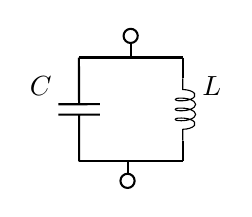
\begin{tikzpicture}[x=0.75pt,y=0.75pt,yscale=-1,xscale=1]
%uncomment if require: \path (0,97); %set diagram left start at 0, and has height of 97

%Shape: Capacitor [id:dp4670171494463129] 
\draw  [line width=0.75]  (50,23.83) -- (50.05,46.33) (60.07,51.31) -- (40.07,51.36) (60.05,46.31) -- (40.05,46.36) (50.07,51.33) -- (50.12,73.83) ;
%Straight Lines [id:da7530368359567341] 
\draw [line width=0.75]    (50,23.83) -- (100,23.83) ;
%Straight Lines [id:da37073903294106214] 
\draw [line width=0.75]    (50,73.83) -- (100,73.83) ;
%Straight Lines [id:da6760299644418128] 
\draw [line width=0.75]    (100,23.83) -- (100,33.83) ;
%Straight Lines [id:da16342394128001536] 
\draw [line width=0.75]    (100,63.83) -- (100,73.83) ;
%Straight Lines [id:da10569605743197075] 
\draw [line width=0.75]    (73.42,79.83) -- (73.42,73.83) ;
%Shape: Circle [id:dp3114709006095975] 
\draw  [line width=0.75]  (70,83.25) .. controls (70,81.36) and (71.53,79.83) .. (73.42,79.83) .. controls (75.3,79.83) and (76.83,81.36) .. (76.83,83.25) .. controls (76.83,85.14) and (75.3,86.67) .. (73.42,86.67) .. controls (71.53,86.67) and (70,85.14) .. (70,83.25) -- cycle ;
%Straight Lines [id:da44379321850243414] 
\draw [line width=0.75]    (75,16.83) -- (75,23.83) ;
%Shape: Circle [id:dp37786908957841614] 
\draw  [line width=0.75]  (78.33,13.33) .. controls (78.38,15.22) and (76.89,16.78) .. (75,16.83) .. controls (73.11,16.88) and (71.55,15.39) .. (71.5,13.5) .. controls (71.45,11.62) and (72.94,10.05) .. (74.83,10) .. controls (76.71,9.95) and (78.28,11.44) .. (78.33,13.33) -- cycle ;
%Shape: Inductor (Air Core) [id:dp009772684946594334] 
\draw   (100,33.83) -- (100,39.23) .. controls (102.63,39.31) and (104.87,40.06) .. (105.66,41.12) .. controls (106.44,42.18) and (105.61,43.34) .. (103.55,44.03) .. controls (101.95,44.57) and (99.88,44.79) .. (97.87,44.63) .. controls (97.08,44.63) and (96.45,44.36) .. (96.45,44.03) .. controls (96.45,43.7) and (97.08,43.43) .. (97.87,43.43) .. controls (99.88,43.28) and (101.95,43.5) .. (103.55,44.03) .. controls (105.26,44.66) and (106.23,45.52) .. (106.23,46.43) .. controls (106.23,47.34) and (105.26,48.21) .. (103.55,48.83) .. controls (101.95,49.37) and (99.88,49.59) .. (97.87,49.43) .. controls (97.08,49.43) and (96.45,49.16) .. (96.45,48.83) .. controls (96.45,48.5) and (97.08,48.23) .. (97.87,48.23) .. controls (99.88,48.08) and (101.95,48.3) .. (103.55,48.83) .. controls (105.26,49.46) and (106.23,50.32) .. (106.23,51.23) .. controls (106.23,52.14) and (105.26,53.01) .. (103.55,53.63) .. controls (101.95,54.17) and (99.88,54.39) .. (97.87,54.23) .. controls (97.08,54.23) and (96.45,53.96) .. (96.45,53.63) .. controls (96.45,53.3) and (97.08,53.03) .. (97.87,53.03) .. controls (99.88,52.88) and (101.95,53.1) .. (103.55,53.63) .. controls (105.61,54.33) and (106.44,55.48) .. (105.66,56.54) .. controls (104.87,57.61) and (102.63,58.35) .. (100,58.43) -- (100,63.83) ;

% Text Node
\draw (108.23,43.43) node [anchor=south west] [inner sep=0.75pt]   [align=left] {$\displaystyle L$};
% Text Node
\draw (38.05,43.36) node [anchor=south east] [inner sep=0.75pt]   [align=left] {$\displaystyle C$};


\end{tikzpicture}
        \vspace{-0.7cm}
        \caption{Circuit diagram of LC resonator}
        \label{fig:LC}
    \end{minipage}
    \hfill
    \begin{minipage}[b]{0.45\linewidth}
      \centering
      

\tikzset{every picture/.style={line width=0.75pt}} %set default line width to 0.75pt        

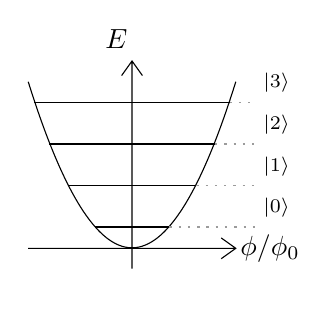
\begin{tikzpicture}[x=0.75pt,y=0.75pt,yscale=-1,xscale=1]
%uncomment if require: \path (0,200); %set diagram left start at 0, and has height of 200

%Shape: Parabola [id:dp37890511708987873] 
\draw   (60,70) .. controls (93.33,176.67) and (126.67,176.67) .. (160,70) ;
%Shape: Axis 2D [id:dp3773695523891737] 
\draw  (60,150.25) -- (160,150.25)(110,60) -- (110,160) (153,145.25) -- (160,150.25) -- (153,155.25) (105,67) -- (110,60) -- (115,67)  ;
%Straight Lines [id:da3077075366408746] 
\draw    (92,140) -- (128,140) ;
%Straight Lines [id:da2626121978197561] 
\draw    (79,120) -- (141,120) ;
%Straight Lines [id:da8498237157026597] 
\draw    (70,100) -- (150,100) ;
%Straight Lines [id:da16494940971997396] 
\draw    (63,80) -- (157,80) ;
%Straight Lines [id:da15643784358380952] 
\draw [color={rgb, 255:red, 155; green, 155; blue, 155 }  ,draw opacity=1 ] [dash pattern={on 0.84pt off 2.51pt}]  (128,140) -- (170,140) ;
%Straight Lines [id:da7225933392434986] 
\draw [color={rgb, 255:red, 155; green, 155; blue, 155 }  ,draw opacity=1 ] [dash pattern={on 0.84pt off 2.51pt}]  (141,120) -- (170,120) ;
%Straight Lines [id:da6235512774693245] 
\draw [color={rgb, 255:red, 155; green, 155; blue, 155 }  ,draw opacity=1 ] [dash pattern={on 0.84pt off 2.51pt}]  (150,100) -- (170,100) ;
%Straight Lines [id:da04257430271569573] 
\draw [color={rgb, 255:red, 155; green, 155; blue, 155 }  ,draw opacity=1 ] [dash pattern={on 0.84pt off 2.51pt}]  (157,80) -- (170,80) ;

% Text Node
\draw (109,49.5) node [anchor=east] [inner sep=0.75pt]   [align=left] {$\displaystyle E$};
% Text Node
\draw (161,142.4) node [anchor=north west][inner sep=0.75pt]    {$\phi /\phi _{0}$};
% Text Node
\draw (172,136.6) node [anchor=south west] [inner sep=0.75pt]  [font=\scriptsize]  {$| 0\rangle $};
% Text Node
\draw (172,116.6) node [anchor=south west] [inner sep=0.75pt]  [font=\scriptsize]  {$| 1\rangle $};
% Text Node
\draw (172,96.6) node [anchor=south west] [inner sep=0.75pt]  [font=\scriptsize]  {$| 2\rangle $};
% Text Node
\draw (172,76.6) node [anchor=south west] [inner sep=0.75pt]  [font=\scriptsize]  {$| 3\rangle $};


\end{tikzpicture}
      \vspace{-1.5cm}
      \caption{Energy spectrum of LC resonator}
      \label{fig:Energy_spectrum}
    \end{minipage}
  \end{figure}
The circuit diagram is illustrated in \cref{fig:LC}, depicting a system that emulates the behavior of a quantum oscillator.
In classical physics, the Hamiltonian for a harmonic oscillator is expressed as follows:
\begin{equation}
    H = \frac{\phi^2}{2L} + \frac{Q^2}{2C},
\end{equation}
where $\phi$ represents the flux in the inductor, and $Q$ denotes the charge on the capacitor.

Quantizing this classical Hamiltonian involves replacing $\phi$ and $Q$ with the flux operator ($\hat{\phi}$) and charge operator ($\hat{Q}$), respectively.
The resulting quantum Hamiltonian, expressed in second quantization form, is given by:
\begin{equation}
    \hat{H} = \frac{\hat{\phi}^2}{2L} + \frac{\hat{Q}^2}{2C} = \hbar \omega \left(\hat{a}^\dagger \hat{a} + \frac{1}{2}\right),
\end{equation}
where $\omega = 1/\sqrt{LC}$ is the resonance frequency of the circuit.
The operators $\hat{a}^\dagger$ and $\hat{a}$ correspond to the creation and annihilation operators of excitations, respectively. 
In this scenario, the excitations represent the difference in the number of charges between the two plates of the capacitor.
Utilizing this quantum description of the LC circuit, we obtain the energy spectrum illustrated in \cref{fig:Energy_spectrum} ($\phi_0 = h/2e$ is the flux quantum) .
The quantization of energy levels in relation to the magnetic flux $\phi$ is clearly evident in the figure.

\subsection{The transmon resonator}

The issue of energy level harmonicity poses a challenge when aiming to construct a quantum processor. 
In this context, determining the specific transitions being driven becomes uncertain, as the energy differences between consecutive levels remain identical.
To address this, we introduce non-linearity into our circuit through the incorporation of the Josephson junction \cite{JOSEPHSON}.

Josephson demonstrated that a current without dissipation could flow between two superconducting electrodes when separated by a thin insulating barrier. Specifically, he established that this supercurrent is determined by
\begin{equation}
    I = I_c \sin(\varphi),
\end{equation}
where $I_c$ represents the critical current of the junction, and $\varphi$ denotes the phase difference between the superconducting condensates on each side of the junction.
\begin{figure}
    \begin{minipage}[b]{0.5\linewidth}
      \centering
        

\tikzset{every picture/.style={line width=0.75pt}} %set default line width to 0.75pt        

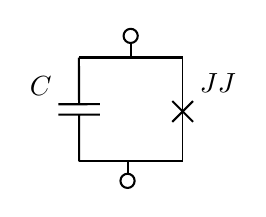
\begin{tikzpicture}[x=0.75pt,y=0.75pt,yscale=-1,xscale=1]
%uncomment if require: \path (0,97); %set diagram left start at 0, and has height of 97

%Shape: Capacitor [id:dp8072216489364277] 
\draw  [line width=0.75]  (60,23.83) -- (60.05,46.33) (70.07,51.31) -- (50.07,51.36) (70.05,46.31) -- (50.05,46.36) (60.07,51.33) -- (60.12,73.83) ;
%Straight Lines [id:da183774352314787] 
\draw [line width=0.75]    (105,54.83) -- (115,44.83) ;
%Straight Lines [id:da1896922658483372] 
\draw [line width=0.75]    (105,44.83) -- (115,54.83) ;

%Straight Lines [id:da33699096520016336] 
\draw [line width=0.75]    (60,23.83) -- (110,23.83) ;
%Straight Lines [id:da6915014186556621] 
\draw [line width=0.75]    (60,73.83) -- (110,73.83) ;
%Straight Lines [id:da36159548727595725] 
\draw [line width=0.75]    (83.42,79.83) -- (83.42,73.83) ;
%Shape: Circle [id:dp8015144235751568] 
\draw  [line width=0.75]  (80,83.25) .. controls (80,81.36) and (81.53,79.83) .. (83.42,79.83) .. controls (85.3,79.83) and (86.83,81.36) .. (86.83,83.25) .. controls (86.83,85.14) and (85.3,86.67) .. (83.42,86.67) .. controls (81.53,86.67) and (80,85.14) .. (80,83.25) -- cycle ;
%Straight Lines [id:da3714464315940995] 
\draw [line width=0.75]    (85,16.83) -- (85,23.83) ;
%Shape: Circle [id:dp25364190410803145] 
\draw  [line width=0.75]  (88.33,13.33) .. controls (88.38,15.22) and (86.89,16.78) .. (85,16.83) .. controls (83.11,16.88) and (81.55,15.39) .. (81.5,13.5) .. controls (81.45,11.62) and (82.94,10.05) .. (84.83,10) .. controls (86.71,9.95) and (88.28,11.44) .. (88.33,13.33) -- cycle ;
%Straight Lines [id:da8131700138845456] 
\draw    (110,23.83) -- (110,73.83) ;

% Text Node
\draw (48.05,43.36) node [anchor=south east] [inner sep=0.75pt]   [align=left] {$\displaystyle C$};
% Text Node
\draw (117,41.83) node [anchor=south west] [inner sep=0.75pt]   [align=left] {$\displaystyle JJ$};


\end{tikzpicture}
        \vspace{-0.8cm}
        \caption{Circuit diagram of a transmon resonator}
        \label{fig:JJ_circuit}
    \end{minipage}
    \hfill
    \begin{minipage}[b]{0.45\linewidth}
      \centering
      

\tikzset{every picture/.style={line width=0.75pt}} %set default line width to 0.75pt        

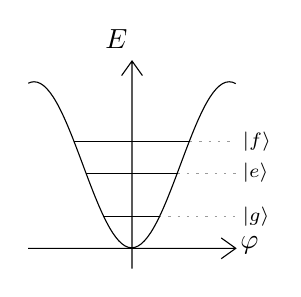
\begin{tikzpicture}[x=0.75pt,y=0.75pt,yscale=-1,xscale=1]
%uncomment if require: \path (0,200); %set diagram left start at 0, and has height of 200

%Straight Lines [id:da03495800698048135] 
\draw [color={rgb, 255:red, 155; green, 155; blue, 155 }  ,draw opacity=1 ] [dash pattern={on 0.84pt off 2.51pt}]  (123,135) -- (160,135) ;
%Shape: Axis 2D [id:dp2373273044965445] 
\draw  (60,150.25) -- (160,150.25)(110,60) -- (110,160) (153,145.25) -- (160,150.25) -- (153,155.25) (105,67) -- (110,60) -- (115,67)  ;
%Shape: Wave [id:dp12933752750229321] 
\draw   (60,70.71) .. controls (60.93,70.25) and (61.87,70) .. (62.82,70) .. controls (71.32,70) and (78.66,89.51) .. (86.32,110) .. controls (93.98,130.49) and (101.32,150) .. (109.82,150) .. controls (118.32,150) and (125.66,130.49) .. (133.32,110) .. controls (140.98,89.51) and (148.32,70) .. (156.82,70) .. controls (157.9,70) and (158.96,70.31) .. (160,70.9) ;
%Straight Lines [id:da530045401686506] 
\draw    (96,135) -- (123,135) ;
%Straight Lines [id:da34934240050097976] 
\draw    (88,114) -- (132,114) ;
%Straight Lines [id:da19311872891258342] 
\draw    (82,99) -- (138,99) ;
%Straight Lines [id:da3065730660397551] 
\draw [color={rgb, 255:red, 155; green, 155; blue, 155 }  ,draw opacity=1 ] [dash pattern={on 0.84pt off 2.51pt}]  (132,114) -- (160,114) ;
%Straight Lines [id:da057644743938617404] 
\draw [color={rgb, 255:red, 155; green, 155; blue, 155 }  ,draw opacity=1 ] [dash pattern={on 0.84pt off 2.51pt}]  (138,99) -- (160,99) ;

% Text Node
\draw (109,49.5) node [anchor=east] [inner sep=0.75pt]   [align=left] {$\displaystyle E$};
% Text Node
\draw (161,143.4) node [anchor=north west][inner sep=0.75pt]    {$\varphi $};
% Text Node
\draw (162,135) node [anchor=west] [inner sep=0.75pt]  [font=\scriptsize]  {$|g\rangle $};
% Text Node
\draw (162,114) node [anchor=west] [inner sep=0.75pt]  [font=\scriptsize]  {$|e\rangle $};
% Text Node
\draw (162,99) node [anchor=west] [inner sep=0.75pt]  [font=\scriptsize]  {$|f\rangle $};


\end{tikzpicture}
      \vspace{-1.2cm}
      \caption{Energy spectrum of transmon resonator}
      \label{fig:Energy_spectrum_JJ}
    \end{minipage}
  \end{figure}

By replacing the inductor of the LC resonator with a Josephson junction (\cref{fig:JJ_circuit}), we achieve the desired anharmonicity of the energy levels.
The resulting potential becomes a cosine potential, leading to non-equidistant energy levels, as illustrated in \cref{fig:Energy_spectrum_JJ}.
To gain a deeper insight into the origin of this anharmonicity, we present the Hamiltonian of the Josephson junction resonator in second quantization formalism:
\begin{equation}
\label{eq:cosina_H}
    \hat{H} = 
    \hbar \omega \hat{a}^\dagger \hat{a} - 
    \frac{E_C}{2}\hat{a}^\dagger\hat{a}^\dagger\hat{a}\hat{a} ,
\end{equation}
where
\begin{equation}
    E_C = \frac{e^2}{2 C_\Sigma}
\end{equation} 
is the charging energy and $C_\Sigma = C_J + C_C$ is the total capacitance.
The Hamiltonian described in \cref{eq:cosina_H} essentially represents an harmonic oscillator incorporating an anharmonicity correction. 
This allows us to address individual energy levels separately.

This arrangement is employed in quantum computation, utilizing the first two energy levels, $\ket{g}$ and $\ket{e}$, for encoding quantum state information. 
Typically, the $\ket{f}$ state is utilized as an auxiliary energy level during the implementation of certain operations.

In our laboratory, the transmon qubit is realized through the Josephson junction resonator under specific conditions known as the \emph{transmon regime} \cite{transmon_regime}.

An advantageous adaptation of the transmon artificial atom is the flux-tunable transmon, in which the single Josephson junction is substituted with two parallel junctions, forming a superconducting quantum interference device (SQUID).
\begin{figure}
    \begin{minipage}[b]{0.5\linewidth}
      \centering
      


\tikzset{every picture/.style={line width=0.75pt}} %set default line width to 0.75pt        

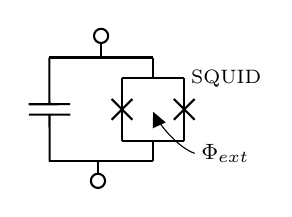
\begin{tikzpicture}[x=0.75pt,y=0.75pt,yscale=-1,xscale=1]
%uncomment if require: \path (0,97); %set diagram left start at 0, and has height of 97

%Shape: Capacitor [id:dp34366919102472526] 
\draw  [line width=0.75]  (20,23.83) -- (20.05,46.33) (30.07,51.31) -- (10.07,51.36) (30.05,46.31) -- (10.05,46.36) (20.07,51.33) -- (20.12,73.83) ;
%Straight Lines [id:da9532858123226031] 
\draw [line width=0.75]    (55,33.83) -- (85,33.83) ;
%Straight Lines [id:da4790035249190253] 
\draw [line width=0.75]    (85,33.83) -- (85,63.83) ;
%Straight Lines [id:da5192559786668693] 
\draw [line width=0.75]    (55,33.83) -- (55,63.83) ;
%Straight Lines [id:da23389027703175358] 
\draw [line width=0.75]    (55,63.83) -- (85,63.83) ;
%Straight Lines [id:da6028752523424945] 
\draw [line width=0.75]    (50,43.83) -- (60,53.83) ;
%Straight Lines [id:da22268293223346158] 
\draw [line width=0.75]    (50,53.83) -- (60,43.83) ;
%Straight Lines [id:da7666685944565205] 
\draw [line width=0.75]    (80,53.83) -- (90,43.83) ;
%Straight Lines [id:da0860971350076063] 
\draw [line width=0.75]    (80,43.83) -- (90,53.83) ;
%Straight Lines [id:da32147396047949894] 
\draw [line width=0.75]    (20,23.83) -- (70,23.83) ;
%Straight Lines [id:da3842851758264739] 
\draw [line width=0.75]    (20,73.83) -- (70,73.83) ;
%Straight Lines [id:da04257544936461244] 
\draw [line width=0.75]    (70,23.83) -- (70,33.83) ;
%Straight Lines [id:da22754146049716317] 
\draw [line width=0.75]    (70,63.83) -- (70,73.83) ;
%Straight Lines [id:da6459112049306985] 
\draw [line width=0.75]    (43.42,79.83) -- (43.42,73.83) ;
%Shape: Circle [id:dp6531205659740902] 
\draw  [line width=0.75]  (40,83.25) .. controls (40,81.36) and (41.53,79.83) .. (43.42,79.83) .. controls (45.3,79.83) and (46.83,81.36) .. (46.83,83.25) .. controls (46.83,85.14) and (45.3,86.67) .. (43.42,86.67) .. controls (41.53,86.67) and (40,85.14) .. (40,83.25) -- cycle ;
%Straight Lines [id:da42435820900303667] 
\draw [line width=0.75]    (45,16.83) -- (45,23.83) ;
%Shape: Circle [id:dp32456243319283773] 
\draw  [line width=0.75]  (48.33,13.33) .. controls (48.38,15.22) and (46.89,16.78) .. (45,16.83) .. controls (43.11,16.88) and (41.55,15.39) .. (41.5,13.5) .. controls (41.45,11.62) and (42.94,10.05) .. (44.83,10) .. controls (46.71,9.95) and (48.28,11.44) .. (48.33,13.33) -- cycle ;

%Curve Lines [id:da7487363329577509] 
\draw [color={rgb, 255:red, 0; green, 0; blue, 0 }  ,draw opacity=1 ]   (90,70) .. controls (83.25,67.65) and (75.22,59.11) .. (71.34,52.55) ;
\draw [shift={(70,50)}, rotate = 65.77] [fill={rgb, 255:red, 0; green, 0; blue, 0 }  ,fill opacity=1 ][line width=0.08]  [draw opacity=0] (7.14,-3.43) -- (0,0) -- (7.14,3.43) -- cycle    ;

% Text Node
\draw (87,33.83) node [anchor=west] [inner sep=0.75pt]   [align=left] {{\scriptsize SQUID}};
% Text Node
\draw (92,70) node [anchor=west] [inner sep=0.75pt]  [font=\footnotesize,color={rgb, 255:red, 0; green, 0; blue, 0 }  ,opacity=1 ] [align=left] {$\displaystyle \Phi _{\text{ext}}$};


\end{tikzpicture}
      \captionsetup{skip=-20pt}
      \caption{Circuit diagram of a flux-tunable transmon}
      \label{fig:transmon_circuit}
    \end{minipage}
    \hfill
    \begin{minipage}[b]{0.45\linewidth}
      \centering
      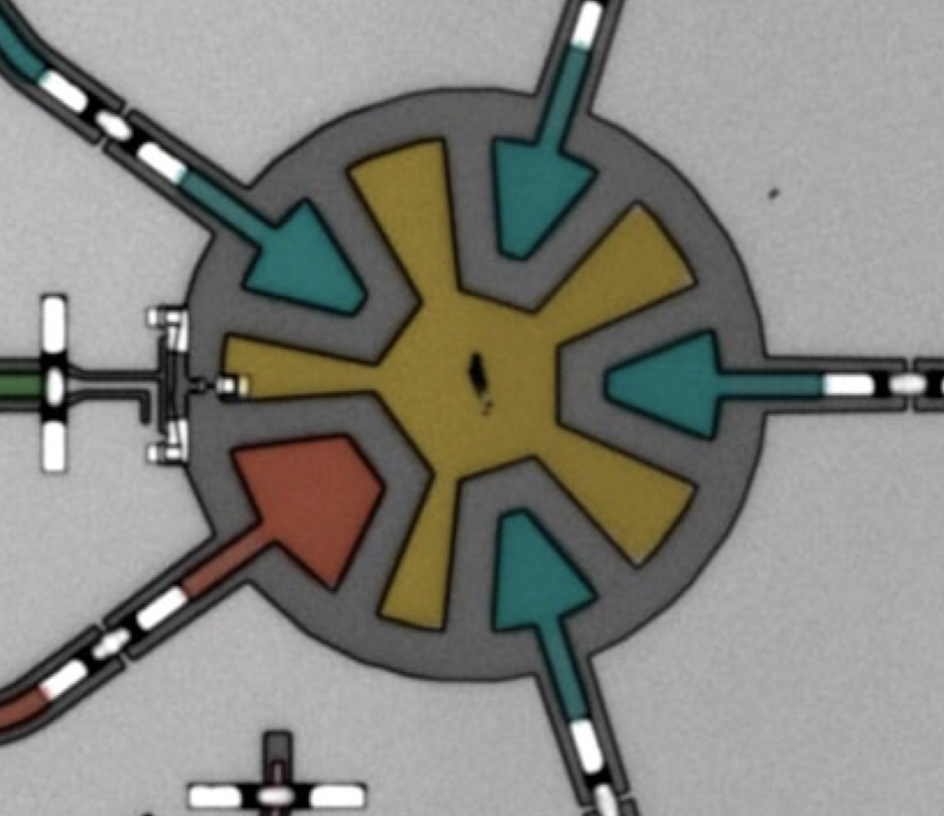
\includegraphics[width = 0.5 \textwidth]{Images/Chap1/star_transmon.png}
      \caption{Star-shaped transmon qubit}
      \label{fig:star_transmon}
    \end{minipage}
  \end{figure}

Replacing the Josephson junction with a SQUID loop introduces a flux-dependent Josephson energy, $E_J(\Phi_\text{ext})$ (see \cref{fig:transmon_circuit}).
Consequently, this results in a flux-tunable transmon frequency 
\begin{equation}
    \omega_q(\Phi_\text{ext}) = \sqrt{8 E_C|E_J(\Phi_\text{ext})|} - E_C/\hbar^3.
\end{equation}
In practical terms, the transmon frequency can be dynamically tuned by up to $\SI{1}{\giga\hertz}$ \cite{di_carlo}.
The magnetic flux within the SQUID loop is produced and regulated by the current flowing through the \emph{flux line}, a nearby waveguide adjacent to the SQUID loop.

In our laboratory, we employ star-shaped transmon qubits \cite{transmon_qubits}, similar to the one depicted in \cref{fig:star_transmon}.
These qubits feature a SQUID loop, making them flux tunable.




%\section{Dispersive Readout}
\label{sec:readout}

The readout mechanism allows us to measure the state of the qubit in a non-demolishing way \cite{singleshot_readout}.
In our experiments this is needed in order to characterize the device and for calibration purposes.

The transmon our capacitively coupled to a readout resonator, which is a waveguide on our device.
By sending through this waveguide a signal far detuned from the qubit's frequency, its frequency will slightly change depending on the state of the qubit, without interfering with the state of the latter.
This process ids described by the James-Cummins Hamiltonian
\begin{equation}
    \hat{H} = \hbar \omega_r \hat{a}^\dagger \hat{a} + \frac{1}{2} \hbar \omega_{ge} \hat{\sigma}^z + \hbar g (\hat{a}^\dagger \hat{\sigma}^- + \hat{a} \hat{\sigma}^+) ,
\end{equation}
which models the coupling between a 2-level system and a light mode in a cavity.
Thus, by measuring the frequency shift of the readout resonator, we are able to infer the qubit's state.

In order to not let the qubit couple too strongly to the environment through the readout resonator, a Purcell filter is applied between the resonator and the qubit (see \cref{fig:diagram_storage_qubit}).
This allows to keep the lifetimes of the qubits longer, by suppressing spontaneous emission due to the Purcell effect \cite{Purcell_effect}.

\begin{figure}
    \centering
    

\tikzset{every picture/.style={line width=0.75pt}} %set default line width to 0.75pt      

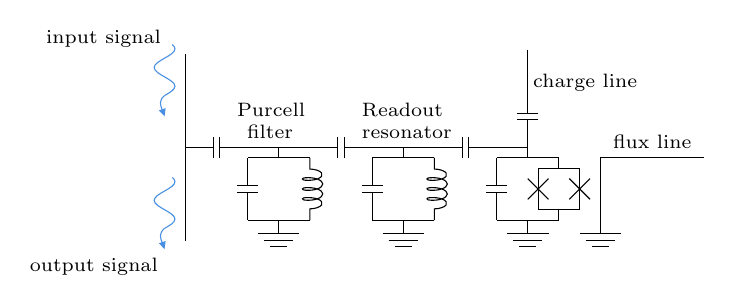
\begin{tikzpicture}[x=0.75pt,y=0.75pt,yscale=-1,xscale=1]
%uncomment if require: \path (0,300); %set diagram left start at 0, and has height of 300

%Shape: Capacitor [id:dp6229484510249941] 
\draw   (80,115) -- (93.5,115) (96.5,110) -- (96.5,120) (93.5,110) -- (93.5,120) (96.5,115) -- (110,115) ;
%Straight Lines [id:da5079772797363618] 
\draw    (140,120) -- (110,120) ;
%Shape: Inductor (Air Core) [id:dp10839806036975186] 
\draw   (140,120) -- (140,125.4) .. controls (142.63,125.48) and (144.87,126.23) .. (145.66,127.29) .. controls (146.44,128.35) and (145.61,129.5) .. (143.55,130.2) .. controls (141.95,130.74) and (139.88,130.95) .. (137.87,130.8) .. controls (137.08,130.8) and (136.45,130.53) .. (136.45,130.2) .. controls (136.45,129.87) and (137.08,129.6) .. (137.87,129.6) .. controls (139.88,129.45) and (141.95,129.66) .. (143.55,130.2) .. controls (145.26,130.82) and (146.23,131.69) .. (146.23,132.6) .. controls (146.23,133.51) and (145.26,134.38) .. (143.55,135) .. controls (141.95,135.54) and (139.88,135.75) .. (137.87,135.6) .. controls (137.08,135.6) and (136.45,135.33) .. (136.45,135) .. controls (136.45,134.67) and (137.08,134.4) .. (137.87,134.4) .. controls (139.88,134.25) and (141.95,134.46) .. (143.55,135) .. controls (145.26,135.62) and (146.23,136.49) .. (146.23,137.4) .. controls (146.23,138.31) and (145.26,139.18) .. (143.55,139.8) .. controls (141.95,140.34) and (139.88,140.55) .. (137.87,140.4) .. controls (137.08,140.4) and (136.45,140.13) .. (136.45,139.8) .. controls (136.45,139.47) and (137.08,139.2) .. (137.87,139.2) .. controls (139.88,139.05) and (141.95,139.26) .. (143.55,139.8) .. controls (145.61,140.5) and (146.44,141.65) .. (145.66,142.71) .. controls (144.87,143.77) and (142.63,144.52) .. (140,144.6) -- (140,150) ;
%Shape: Capacitor [id:dp06818692783071034] 
\draw   (110,120) -- (110,133.5) (115,136.5) -- (105,136.5) (115,133.5) -- (105,133.5) (110,136.5) -- (110,150) ;
%Straight Lines [id:da7350026547264685] 
\draw    (110,150) -- (140,150) ;
%Straight Lines [id:da23995913734624486] 
\draw    (80,70) -- (80,160) ;
%Straight Lines [id:da1612492392898659] 
\draw    (110,115) -- (140,115) ;
%Straight Lines [id:da5671640840709973] 
\draw    (125,115) -- (125,120) ;
%Shape: Capacitor [id:dp5438650003798182] 
\draw   (140,115) -- (153.5,115) (156.5,110) -- (156.5,120) (153.5,110) -- (153.5,120) (156.5,115) -- (170,115) ;
%Straight Lines [id:da49049414599623864] 
\draw    (200,120) -- (170,120) ;
%Shape: Inductor (Air Core) [id:dp010409349579149074] 
\draw   (200,120) -- (200,125.4) .. controls (202.63,125.48) and (204.87,126.23) .. (205.66,127.29) .. controls (206.44,128.35) and (205.61,129.5) .. (203.55,130.2) .. controls (201.95,130.74) and (199.88,130.95) .. (197.87,130.8) .. controls (197.08,130.8) and (196.45,130.53) .. (196.45,130.2) .. controls (196.45,129.87) and (197.08,129.6) .. (197.87,129.6) .. controls (199.88,129.45) and (201.95,129.66) .. (203.55,130.2) .. controls (205.26,130.82) and (206.23,131.69) .. (206.23,132.6) .. controls (206.23,133.51) and (205.26,134.38) .. (203.55,135) .. controls (201.95,135.54) and (199.88,135.75) .. (197.87,135.6) .. controls (197.08,135.6) and (196.45,135.33) .. (196.45,135) .. controls (196.45,134.67) and (197.08,134.4) .. (197.87,134.4) .. controls (199.88,134.25) and (201.95,134.46) .. (203.55,135) .. controls (205.26,135.62) and (206.23,136.49) .. (206.23,137.4) .. controls (206.23,138.31) and (205.26,139.18) .. (203.55,139.8) .. controls (201.95,140.34) and (199.88,140.55) .. (197.87,140.4) .. controls (197.08,140.4) and (196.45,140.13) .. (196.45,139.8) .. controls (196.45,139.47) and (197.08,139.2) .. (197.87,139.2) .. controls (199.88,139.05) and (201.95,139.26) .. (203.55,139.8) .. controls (205.61,140.5) and (206.44,141.65) .. (205.66,142.71) .. controls (204.87,143.77) and (202.63,144.52) .. (200,144.6) -- (200,150) ;
%Shape: Capacitor [id:dp38289405277156474] 
\draw   (170,120) -- (170,133.5) (175,136.5) -- (165,136.5) (175,133.5) -- (165,133.5) (170,136.5) -- (170,150) ;
%Straight Lines [id:da7342631646168638] 
\draw    (170,150) -- (200,150) ;
%Shape: Capacitor [id:dp4965705456609162] 
\draw   (200,115) -- (213.5,115) (216.5,110) -- (216.5,120) (213.5,110) -- (213.5,120) (216.5,115) -- (230,115) ;
%Straight Lines [id:da5477595668599946] 
\draw    (170,115) -- (200,115) ;
%Straight Lines [id:da7609436744451872] 
\draw    (185,115) -- (185,120) ;
%Straight Lines [id:da932132356010352] 
\draw    (260,120) -- (230,120) ;
%Shape: Capacitor [id:dp925083204210299] 
\draw   (230,120) -- (230,133.5) (235,136.5) -- (225,136.5) (235,133.5) -- (225,133.5) (230,136.5) -- (230,150) ;
%Straight Lines [id:da48756322841661204] 
\draw    (230,150) -- (260,150) ;
%Straight Lines [id:da9662762169593431] 
\draw    (245,115) -- (245,120) ;
%Straight Lines [id:da607486087129423] 
\draw    (250,125) -- (270,125) ;
%Straight Lines [id:da4269839144692542] 
\draw    (250,145) -- (270,145) ;
%Straight Lines [id:da6212379775483154] 
\draw    (270,125) -- (270,145) ;
%Straight Lines [id:da42941601462568646] 
\draw    (250,125) -- (250,145) ;
%Straight Lines [id:da9671029825944342] 
\draw    (260,120) -- (260,125) ;
%Straight Lines [id:da9712181495027408] 
\draw    (260,145) -- (260,150) ;
%Straight Lines [id:da3624697790998732] 
\draw    (265,130) -- (275,140) ;
%Straight Lines [id:da4335724022567018] 
\draw    (245,130) -- (255,140) ;
%Straight Lines [id:da530417781084312] 
\draw    (255,130) -- (245,140) ;
%Straight Lines [id:da9581131846208597] 
\draw    (275,130) -- (265,140) ;
%Straight Lines [id:da038301723534536425] 
\draw    (230,115) -- (245,115) ;
%Shape: Ground [id:dp6910953506421662] 
\draw   (115,156.67) -- (135,156.67) ;
\draw   (118,159.67) -- (132,159.67) ;
\draw   (121,162.67) -- (129,162.67) ;
\draw   (125,150) -- (125,156.67) ;
%Shape: Ground [id:dp4840755871676472] 
\draw   (175,156.67) -- (195,156.67) ;
\draw   (178,159.67) -- (192,159.67) ;
\draw   (181,162.67) -- (189,162.67) ;
\draw   (185,150) -- (185,156.67) ;
%Shape: Ground [id:dp7159028270026297] 
\draw   (235,156.67) -- (255,156.67) ;
\draw   (238,159.67) -- (252,159.67) ;
\draw   (241,162.67) -- (249,162.67) ;
\draw   (245,150) -- (245,156.67) ;
%Straight Lines [id:da07274023253816075] 
\draw    (280,120) -- (330,120) ;
%Straight Lines [id:da0646328748380458] 
\draw    (280,120) -- (280,150) ;
%Shape: Ground [id:dp10990759893272828] 
\draw   (270,156.67) -- (290,156.67) ;
\draw   (273,159.67) -- (287,159.67) ;
\draw   (276,162.67) -- (284,162.67) ;
\draw   (280,150) -- (280,156.67) ;
%Straight Lines [id:da8443452176258857] 
\draw    (245,68) -- (245,85) ;
%Shape: Capacitor [id:dp2673784375807502] 
\draw   (245,85) -- (245,98.5) (250,101.5) -- (240,101.5) (250,98.5) -- (240,98.5) (245,101.5) -- (245,115) ;
%Shape: Wave [id:dp46962992426174544] 
\draw  [color={rgb, 255:red, 74; green, 144; blue, 226 }  ,draw opacity=1 ] (70,90) .. controls (72.56,88.53) and (75,87.13) .. (75,85.5) .. controls (75,83.87) and (72.56,82.47) .. (70,81) .. controls (67.44,79.53) and (65,78.13) .. (65,76.5) .. controls (65,74.87) and (67.44,73.47) .. (70,72) .. controls (72.56,70.53) and (75,69.13) .. (75,67.5) .. controls (75,66.77) and (74.51,66.09) .. (73.75,65.43) ;
%Curve Lines [id:da8193635142444085] 
\draw [color={rgb, 255:red, 74; green, 144; blue, 226 }  ,draw opacity=1 ]   (70,90) .. controls (67.21,92.34) and (67.82,94.25) .. (68.96,97.21) ;
\draw [shift={(70,100)}, rotate = 251.57] [fill={rgb, 255:red, 74; green, 144; blue, 226 }  ,fill opacity=1 ][line width=0.08]  [draw opacity=0] (3.57,-1.72) -- (0,0) -- (3.57,1.72) -- cycle    ;
%Shape: Wave [id:dp5292058745377288] 
\draw  [color={rgb, 255:red, 74; green, 144; blue, 226 }  ,draw opacity=1 ] (70,154) .. controls (72.56,152.53) and (75,151.13) .. (75,149.5) .. controls (75,147.87) and (72.56,146.47) .. (70,145) .. controls (67.44,143.53) and (65,142.13) .. (65,140.5) .. controls (65,138.87) and (67.44,137.47) .. (70,136) .. controls (72.56,134.53) and (75,133.13) .. (75,131.5) .. controls (75,130.77) and (74.51,130.09) .. (73.75,129.43) ;
%Curve Lines [id:da04097203302843688] 
\draw [color={rgb, 255:red, 74; green, 144; blue, 226 }  ,draw opacity=1 ]   (70,154) .. controls (67.21,156.34) and (67.82,158.25) .. (68.96,161.21) ;
\draw [shift={(70,164)}, rotate = 251.57] [fill={rgb, 255:red, 74; green, 144; blue, 226 }  ,fill opacity=1 ][line width=0.08]  [draw opacity=0] (3.57,-1.72) -- (0,0) -- (3.57,1.72) -- cycle    ;

% Text Node
\draw (305,117) node [anchor=south] [inner sep=0.75pt]  [font=\scriptsize] [align=left] {{\scriptsize flux line}};
% Text Node
\draw (246.31,83.64) node [anchor=west] [inner sep=0.75pt]  [font=\scriptsize] [align=left] {{\scriptsize charge line}};
% Text Node
\draw (181,112) node [anchor=south] [inner sep=0.75pt]  [font=\scriptsize] [align=left] {\begin{minipage}[lt]{23.84pt}\setlength\topsep{0pt}
\begin{center}
{\scriptsize Readout}\\{\scriptsize resonator }
\end{center}

\end{minipage}};
% Text Node
\draw (138,112) node [anchor=south east] [inner sep=0.75pt]  [font=\scriptsize] [align=left] {\begin{minipage}[lt]{23.84pt}\setlength\topsep{0pt}
\begin{center}
{\scriptsize Purcell}\\{\scriptsize filter}
\end{center}

\end{minipage}};
% Text Node
\draw (69.47,67.86) node [anchor=south east] [inner sep=0.75pt]  [font=\scriptsize] [align=left] {{\scriptsize input signal}};
% Text Node
\draw (68,167) node [anchor=north east] [inner sep=0.75pt]  [font=\scriptsize] [align=left] {{\scriptsize output signal}};


\end{tikzpicture}


    \vspace{-1cm}
    \caption{Diagram representing a storage qubit and their readout mechanism}
    \label{fig:diagram_storage_qubit}
\end{figure}

\section{Tunable Couplers}
\label{sec:tunable_couplers}

Qubits in our device are coupled through tunable couplers.
They allow us to mediate interaction between the qubits and perform two-qubits gates.
They are composed of two planar waveguide, one of them with a fixed coupling term $J_{\text{fixed}}$.
The other is instead flux tunable, meaning that its coupling term $J_{\text{tunable}}(\Phi)$ can be tuned with the magnetic flux generated by a flux line and going into a SQUID loop placed on the waveguide as depicted in \cref{fig:tun_coupl}.

\begin{figure}
    \centering
    

\tikzset{every picture/.style={line width=0.75pt}} %set default line width to 0.75pt        

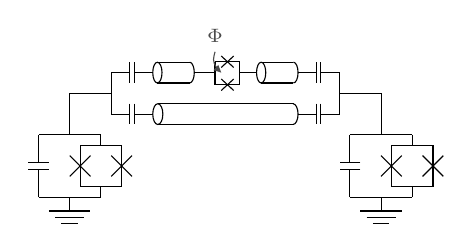
\begin{tikzpicture}[x=0.75pt,y=0.75pt,yscale=-1,xscale=1]
%uncomment if require: \path (0,300); %set diagram left start at 0, and has height of 300

%Straight Lines [id:da07218492708859259] 
\draw    (165,140) -- (135,140) ;
%Shape: Capacitor [id:dp26518043172092054] 
\draw   (135,140) -- (135,153.5) (140,156.5) -- (130,156.5) (140,153.5) -- (130,153.5) (135,156.5) -- (135,170) ;
%Straight Lines [id:da13302415031214743] 
\draw    (135,170) -- (165,170) ;
%Straight Lines [id:da17130629114618245] 
\draw    (155,145) -- (175,145) ;
%Straight Lines [id:da29260280538604033] 
\draw    (155,165) -- (175,165) ;
%Straight Lines [id:da49230231307780326] 
\draw    (175,145) -- (175,165) ;
%Straight Lines [id:da3653947605727903] 
\draw    (155,145) -- (155,165) ;
%Straight Lines [id:da44803766219329755] 
\draw    (165,140) -- (165,145) ;
%Straight Lines [id:da9101556277746032] 
\draw    (165,165) -- (165,170) ;
%Straight Lines [id:da006475878830819681] 
\draw    (170,150) -- (180,160) ;
%Straight Lines [id:da33120831736226397] 
\draw    (150,150) -- (160,160) ;
%Straight Lines [id:da11004761294731558] 
\draw    (160,150) -- (150,160) ;
%Straight Lines [id:da9445264009597942] 
\draw    (180,150) -- (170,160) ;
%Shape: Ground [id:dp22167919288849824] 
\draw   (140, 176.67) -- (160, 176.67) ;
\draw   (143, 179.67) -- (157, 179.67) ;
\draw   (146, 182.67) -- (154, 182.67) ;
\draw   (150, 170) -- (150, 176.67) ;
%Straight Lines [id:da42940827257352] 
\draw    (315,140) -- (285,140) ;
%Shape: Capacitor [id:dp49877304955829627] 
\draw   (285,140) -- (285,153.5) (290,156.5) -- (280,156.5) (290,153.5) -- (280,153.5) (285,156.5) -- (285,170) ;
%Straight Lines [id:da7324100328789034] 
\draw    (285,170) -- (315,170) ;
%Straight Lines [id:da208048098521316] 
\draw    (305,145) -- (325,145) ;
%Straight Lines [id:da8572518030578566] 
\draw    (305,165) -- (325,165) ;
%Straight Lines [id:da5742858039200953] 
\draw    (325,145) -- (325,165) ;
%Straight Lines [id:da3966431831849069] 
\draw    (305,145) -- (305,165) ;
%Straight Lines [id:da19183525795672862] 
\draw    (315,140) -- (315,145) ;
%Straight Lines [id:da004743615923411104] 
\draw    (315,165) -- (315,170) ;
%Straight Lines [id:da17738152912719607] 
\draw    (320,150) -- (330,160) ;
%Straight Lines [id:da8678835567326026] 
\draw    (300,150) -- (310,160) ;
%Straight Lines [id:da28374358820735224] 
\draw    (310,150) -- (300,160) ;
%Straight Lines [id:da24817307713778236] 
\draw    (330,150) -- (320,160) ;
%Shape: Ground [id:dp861700376356459] 
\draw   (290, 176.67) -- (310, 176.67) ;
\draw   (293, 179.67) -- (307, 179.67) ;
\draw   (296, 182.67) -- (304, 182.67) ;
\draw   (300, 170) -- (300, 176.67) ;
%Straight Lines [id:da6625685419222695] 
\draw    (150,140) -- (150,120) ;
%Straight Lines [id:da2635718281625268] 
\draw    (300,140) -- (300,120) ;
%Straight Lines [id:da3980890926472094] 
\draw    (170,120) -- (150,120) ;
%Straight Lines [id:da6516978234304753] 
\draw    (170,120) -- (170,110) ;
%Straight Lines [id:da8682527218489697] 
\draw    (170,130) -- (170,120) ;
%Shape: Capacitor [id:dp26464751353501326] 
\draw   (170,110) -- (179,110) (181,105) -- (181,115) (179,105) -- (179,115) (181,110) -- (190,110) ;
%Shape: Capacitor [id:dp9673816527519772] 
\draw   (170,130) -- (179,130) (181,125) -- (181,135) (179,125) -- (179,135) (181,130) -- (190,130) ;
%Shape: Ellipse [id:dp26511497109868176] 
\draw   (190,110) .. controls (190,107.24) and (191,105) .. (192.22,105) .. controls (193.45,105) and (194.45,107.24) .. (194.45,110) .. controls (194.45,112.76) and (193.45,115) .. (192.22,115) .. controls (191,115) and (190,112.76) .. (190,110) -- cycle ;
%Straight Lines [id:da14470289747688758] 
\draw    (192.22,105) -- (207.79,105) ;
%Straight Lines [id:da773223714503521] 
\draw    (192.22,115) -- (207.79,115) ;
%Shape: Arc [id:dp18440292021788673] 
\draw  [draw opacity=0] (207.79,105) .. controls (209.01,105.02) and (210,107.25) .. (210,110) .. controls (210,112.75) and (209.01,114.98) .. (207.79,115) -- (207.78,110) -- cycle ; \draw   (207.79,105) .. controls (209.01,105.02) and (210,107.25) .. (210,110) .. controls (210,112.75) and (209.01,114.98) .. (207.79,115) ;  

%Shape: Ellipse [id:dp6247106434937635] 
\draw   (190,130) .. controls (190,127.24) and (191.09,125) .. (192.43,125) .. controls (193.77,125) and (194.86,127.24) .. (194.86,130) .. controls (194.86,132.76) and (193.77,135) .. (192.43,135) .. controls (191.09,135) and (190,132.76) .. (190,130) -- cycle ;
%Straight Lines [id:da5902234364980534] 
\draw    (192.43,125) -- (258.06,125) ;
%Straight Lines [id:da6759349880739789] 
\draw    (192.43,135) -- (258.06,135) ;
%Shape: Arc [id:dp6456040885907672] 
\draw  [draw opacity=0] (257.59,125) .. controls (258.92,125.02) and (260,127.25) .. (260,130) .. controls (260,132.75) and (258.92,134.98) .. (257.59,135) -- (257.57,130) -- cycle ; \draw   (257.59,125) .. controls (258.92,125.02) and (260,127.25) .. (260,130) .. controls (260,132.75) and (258.92,134.98) .. (257.59,135) ;  

%Shape: Ellipse [id:dp7275157055864581] 
\draw   (240,110) .. controls (240,107.24) and (241,105) .. (242.22,105) .. controls (243.45,105) and (244.45,107.24) .. (244.45,110) .. controls (244.45,112.76) and (243.45,115) .. (242.22,115) .. controls (241,115) and (240,112.76) .. (240,110) -- cycle ;
%Straight Lines [id:da6315731480773339] 
\draw    (242.22,105) -- (257.79,105) ;
%Straight Lines [id:da6406460700415237] 
\draw    (242.22,115) -- (257.79,115) ;
%Shape: Arc [id:dp38475017613626794] 
\draw  [draw opacity=0] (257.79,105) .. controls (259.01,105.02) and (260,107.25) .. (260,110) .. controls (260,112.75) and (259.01,114.98) .. (257.79,115) -- (257.78,110) -- cycle ; \draw   (257.79,105) .. controls (259.01,105.02) and (260,107.25) .. (260,110) .. controls (260,112.75) and (259.01,114.98) .. (257.79,115) ;  

%Straight Lines [id:da060781913550373545] 
\draw    (210,110) -- (220,110) ;
%Straight Lines [id:da15398066157627577] 
\draw    (232,104.77) -- (232,115.85) ;
%Straight Lines [id:da14222494293706922] 
\draw    (220,104.77) -- (220,115.85) ;
%Straight Lines [id:da6561755710145185] 
\draw    (232,115.85) -- (220,115.85) ;
%Straight Lines [id:da742586164519965] 
\draw    (232,104.77) -- (220,104.77) ;
%Straight Lines [id:da21146645385961227] 
\draw    (229,113.08) -- (223,118.63) ;
%Straight Lines [id:da3871753118676642] 
\draw    (229,102) -- (223,107.54) ;
%Straight Lines [id:da5637422527324993] 
\draw    (229,107.54) -- (223,102) ;
%Straight Lines [id:da9093097576487559] 
\draw    (229,118.63) -- (223,113.08) ;

%Straight Lines [id:da4289728577327423] 
\draw    (232,110) -- (240,110) ;
%Shape: Capacitor [id:dp8421236410162245] 
\draw   (260,110) -- (269,110) (271,105) -- (271,115) (269,105) -- (269,115) (271,110) -- (280,110) ;
%Straight Lines [id:da787480793091047] 
\draw    (280,120) -- (280,110) ;
%Straight Lines [id:da5372127440829679] 
\draw    (280,130) -- (280,120) ;
%Shape: Capacitor [id:dp09893187150822791] 
\draw   (260,130) -- (269,130) (271,125) -- (271,135) (269,125) -- (269,135) (271,130) -- (280,130) ;
%Straight Lines [id:da43455598058651357] 
\draw    (300,120) -- (280,120) ;
%Curve Lines [id:da7527622826730622] 
\draw [color={rgb, 255:red, 74; green, 74; blue, 74 }  ,draw opacity=1 ]   (220,100) .. controls (219.34,102.74) and (218.4,104.58) .. (220.96,107.82) ;
\draw [shift={(223,110)}, rotate = 223.23] [fill={rgb, 255:red, 74; green, 74; blue, 74 }  ,fill opacity=1 ][line width=0.08]  [draw opacity=0] (3.57,-1.72) -- (0,0) -- (3.57,1.72) -- cycle    ;

% Text Node
\draw (220,97) node [anchor=south] [inner sep=0.75pt]  [font=\scriptsize,color={rgb, 255:red, 74; green, 74; blue, 74 }  ,opacity=1 ] [align=left] {$\displaystyle \Phi $};


\end{tikzpicture}
    \vspace{-1cm}
    \caption{Schematic representation of two qubits connected by a tunable coupler}
    \label{fig:tun_coupl}
\end{figure}

The SQUID loop connected to the coupler allows us to control the interaction between the two qubits.
To minimise the interaction between the two qubits and the ZZ crosstalk, the DC flux driving the SQUID loop has to be calibrated to the operation point.

To implement a two-qubit gate, a sinusoidal pulse is sent on top of the DC flux to the SQUID loop.
If the modulation frequency of this pulse matches a transition of the two-qubit system, it will perform a two-qubit gate.
In this way we are able to turn on interactions between specific levels of the qubits.
\textcolor{red}{Reference the next section maybe.}

\chapter{Crosstalk cancellation}
\section{Introduction}
\section{Detection}
\subsection{Rabi-type measurement}
\subsection{Ramsey-type measurement}
\section{Crosstalk calibration}
\section{Verify cancellation}
\chapter{Protocols for 2 qubit gates}
\label{chap:2_qubit_gates}

To execute experiments and induce the emission of entangled photons into the waveguide, conducting both single- and two-qubit gates on our device is essential.
As previously explained in the preceding chapter, conducting single-qubit gates on the emitter qubits is not viable due to their short lifespans.
This limitation also influences the type of two-qubit gate feasible between a storage and an emitter qubit.
For instance, we are unable to perform a controlled-phase gate, or CZ gate, between a storage and an emitter.

In this chapter, we will discuss the types of two-qubit gates that we can perform between storage-storage and storage-emitter qubits.
The gates we are able or unable to perform is the main limiting factor affecting the number of entangled photonic states we can create with our device.

\section{Storage-Emitter operations}
\label{sec:S-E}

In \cref{fig:level_S-E} we illustrate the level diagram for a storage-emitter (S-E) system.
\begin{figure}[h]
    \centering
    

\tikzset{every picture/.style={line width=0.75pt}} %set default line width to 0.75pt        

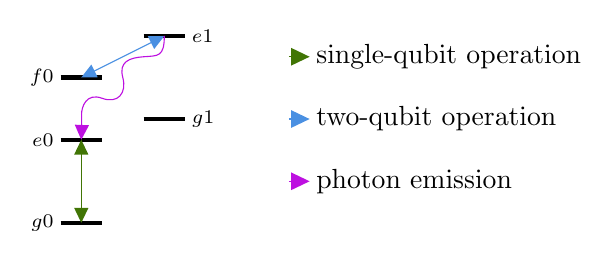
\begin{tikzpicture}[x=0.75pt,y=0.75pt,yscale=-1,xscale=1]
%uncomment if require: \path (0,300); %set diagram left start at 0, and has height of 300

%Straight Lines [id:da9036150792074441] 
\draw [line width=1.5]    (100,100) -- (120,100) ;
%Straight Lines [id:da3892496668455091] 
\draw [line width=1.5]    (140,80) -- (160,80) ;
%Straight Lines [id:da8780144362496497] 
\draw [line width=1.5]    (100,130) -- (120,130) ;
%Straight Lines [id:da9845944648914766] 
\draw [line width=1.5]    (100,170) -- (120,170) ;
%Straight Lines [id:da40423833166537637] 
\draw [line width=1.5]    (140,120) -- (160,120) ;
%Straight Lines [id:da9138884186505395] 
\draw [color={rgb, 255:red, 65; green, 117; blue, 5 }  ,draw opacity=1 ]   (110,133) -- (110,167) ;
\draw [shift={(110,170)}, rotate = 270] [fill={rgb, 255:red, 65; green, 117; blue, 5 }  ,fill opacity=1 ][line width=0.08]  [draw opacity=0] (7.14,-3.43) -- (0,0) -- (7.14,3.43) -- cycle    ;
\draw [shift={(110,130)}, rotate = 90] [fill={rgb, 255:red, 65; green, 117; blue, 5 }  ,fill opacity=1 ][line width=0.08]  [draw opacity=0] (7.14,-3.43) -- (0,0) -- (7.14,3.43) -- cycle    ;
%Straight Lines [id:da18399826038705747] 
\draw [color={rgb, 255:red, 74; green, 144; blue, 226 }  ,draw opacity=1 ]   (147.32,81.34) -- (112.68,98.66) ;
\draw [shift={(110,100)}, rotate = 333.43] [fill={rgb, 255:red, 74; green, 144; blue, 226 }  ,fill opacity=1 ][line width=0.08]  [draw opacity=0] (7.14,-3.43) -- (0,0) -- (7.14,3.43) -- cycle    ;
\draw [shift={(150,80)}, rotate = 153.43] [fill={rgb, 255:red, 74; green, 144; blue, 226 }  ,fill opacity=1 ][line width=0.08]  [draw opacity=0] (7.14,-3.43) -- (0,0) -- (7.14,3.43) -- cycle    ;
%Straight Lines [id:da14000382288661184] 
\draw [color={rgb, 255:red, 65; green, 117; blue, 5 }  ,draw opacity=1 ]   (210,90) -- (217,90) ;
\draw [shift={(220,90)}, rotate = 180] [fill={rgb, 255:red, 65; green, 117; blue, 5 }  ,fill opacity=1 ][line width=0.08]  [draw opacity=0] (8.93,-4.29) -- (0,0) -- (8.93,4.29) -- cycle    ;
%Straight Lines [id:da9331304771806838] 
\draw [color={rgb, 255:red, 74; green, 144; blue, 226 }  ,draw opacity=1 ]   (210,120) -- (217,120) ;
\draw [shift={(220,120)}, rotate = 180] [fill={rgb, 255:red, 74; green, 144; blue, 226 }  ,fill opacity=1 ][line width=0.08]  [draw opacity=0] (8.93,-4.29) -- (0,0) -- (8.93,4.29) -- cycle    ;
%Curve Lines [id:da6855478455179863] 
\draw [color={rgb, 255:red, 189; green, 16; blue, 224 }  ,draw opacity=1 ]   (150,80) .. controls (150,90.17) and (147,89.5) .. (140,90) .. controls (133,90.5) and (128,92.5) .. (130,100) .. controls (132,107.5) and (127.67,112.83) .. (120,110) .. controls (112.33,107.17) and (110.08,114.29) .. (110.13,117.88) .. controls (110.16,120.62) and (110.16,123.77) .. (110.09,127.01) ;
\draw [shift={(110,130)}, rotate = 272.25] [fill={rgb, 255:red, 189; green, 16; blue, 224 }  ,fill opacity=1 ][line width=0.08]  [draw opacity=0] (7.14,-3.43) -- (0,0) -- (7.14,3.43) -- cycle    ;
%Straight Lines [id:da22870453087792075] 
\draw [color={rgb, 255:red, 189; green, 16; blue, 224 }  ,draw opacity=1 ]   (210,150) -- (217,150) ;
\draw [shift={(220,150)}, rotate = 180] [fill={rgb, 255:red, 189; green, 16; blue, 224 }  ,fill opacity=1 ][line width=0.08]  [draw opacity=0] (8.93,-4.29) -- (0,0) -- (8.93,4.29) -- cycle    ;

% Text Node
\draw (98,100) node [anchor=east] [inner sep=0.75pt]  [font=\scriptsize]  {$f0$};
% Text Node
\draw (98,130) node [anchor=east] [inner sep=0.75pt]  [font=\scriptsize]  {$e0$};
% Text Node
\draw (98,170) node [anchor=east] [inner sep=0.75pt]  [font=\scriptsize]  {$g0$};
% Text Node
\draw (162,80) node [anchor=west] [inner sep=0.75pt]  [font=\scriptsize]  {$e1$};
% Text Node
\draw (162,120) node [anchor=west] [inner sep=0.75pt]  [font=\scriptsize]  {$g1$};
% Text Node
\draw (222,90) node [anchor=west] [inner sep=0.75pt]   [align=left] {single-qubit operation};
% Text Node
\draw (222,120) node [anchor=west] [inner sep=0.75pt]   [align=left] {two-qubit operation};
% Text Node
\draw (222,150) node [anchor=west] [inner sep=0.75pt]   [align=left] {photon emission};


\end{tikzpicture}
    \vspace{-1cm}
    \caption{Level diagram of storage-emitter interaction}
    \label{fig:level_S-E}
\end{figure}

We label the levels of the storage qubit with $\ket{g}, \ket{e}, \ket{f}$ and those of the emitter as $\ket{0}, \ket{1}$.
Due to the rapid emission of the emitter, the second excited level $\ket{2}$ is not relevant for our purposes.
In addition, we cannot run single-qubit gates on the emitter.
The only operations we can execute are single-qubit gates on the storage qubit and two-qubit gates that do not require populations to remain coherent in the emitter.
In other words, we can only transfer the excitations from the storage to the emitter.

The two-qubit gates we are able to execute considering the limitations of our device are SWAP and controlled emission (or CNOT).

\subsection{SWAP}


The simplest two-qubit gate executable on an S-E pair is the SWAP gate. 
It maps the storage qubit's state onto the emitter qubit, consequently leading to photon emission through spontaneous decay into the emission line of the ladder.

The unitary matrix representing the SWAP gate is
\begin{equation}
    U_{\text{SWAP}} = 
    \begin{pmatrix}
    1 & 0 & 0 & 0 \\
    0 & 0 & 1 & 0 \\
    0 & 1 & 0 & 0 \\
    0 & 0 & 0 & 1 \\
\end{pmatrix}.
\end{equation}

This implements the operation
\begin{equation}
    \ket{\psi}_{\text{S}} \ket{0}_{\text{E}} \xrightarrow{U_{\text{SWAP}}}
    \ket{g}_{\text{S}} \ket{\psi}_{\text{E}}
\end{equation}
which transfers the quantum state of the storage in the emitter qubit, leaving the former in its ground state.

\begin{figure}
    \centering
    

\tikzset{every picture/.style={line width=0.75pt}} %set default line width to 0.75pt        

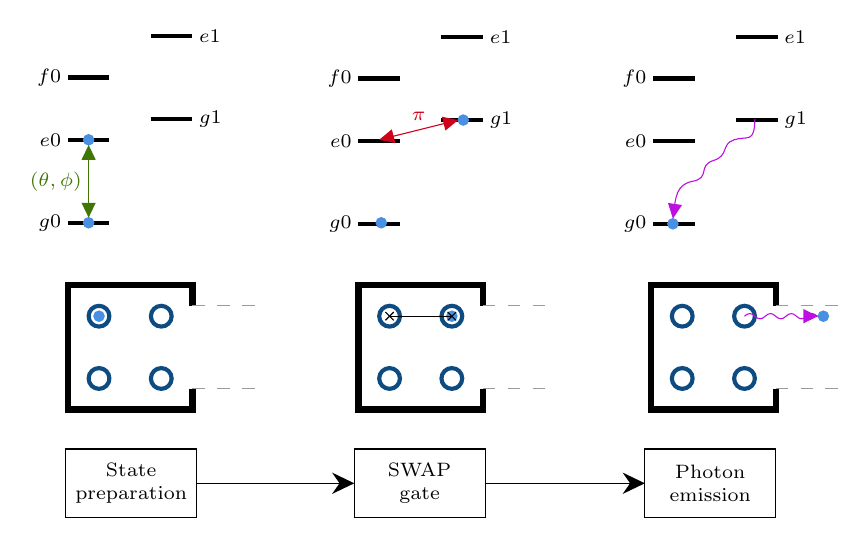
\begin{tikzpicture}[x=0.75pt,y=0.75pt,yscale=-1,xscale=1]
%uncomment if require: \path (0,472); %set diagram left start at 0, and has height of 472

%Straight Lines [id:da8931975658515314] 
\draw [line width=1.5]    (100,100) -- (120,100) ;
%Straight Lines [id:da6109179246921593] 
\draw [line width=1.5]    (140,80) -- (160,80) ;
%Straight Lines [id:da4740245259238267] 
\draw [line width=1.5]    (100,130) -- (120,130) ;
%Straight Lines [id:da8570593937301805] 
\draw [line width=1.5]    (100,170) -- (120,170) ;
%Straight Lines [id:da02915524605611408] 
\draw [line width=1.5]    (140,120) -- (160,120) ;
%Straight Lines [id:da16734412566121315] 
\draw [line width=1.5]    (240,100.5) -- (260,100.5) ;
%Straight Lines [id:da1741824563512493] 
\draw [line width=1.5]    (280,80.5) -- (300,80.5) ;
%Straight Lines [id:da23317779450869036] 
\draw [line width=1.5]    (240,130.5) -- (260,130.5) ;
%Straight Lines [id:da8493304549912968] 
\draw [line width=1.5]    (240,170.5) -- (260,170.5) ;
%Straight Lines [id:da9896717165480059] 
\draw [line width=1.5]    (280,120.5) -- (300,120.5) ;
%Straight Lines [id:da956624069338186] 
\draw [line width=1.5]    (382,100.5) -- (402,100.5) ;
%Straight Lines [id:da7887267818588047] 
\draw [line width=1.5]    (422,80.5) -- (442,80.5) ;
%Straight Lines [id:da03622865125847419] 
\draw [line width=1.5]    (382,130.5) -- (402,130.5) ;
%Straight Lines [id:da13614260982775128] 
\draw [line width=1.5]    (382,170.5) -- (402,170.5) ;
%Straight Lines [id:da1441695211618249] 
\draw [line width=1.5]    (422,120.5) -- (442,120.5) ;
%Shape: Circle [id:dp1759227411497647] 
\draw  [color={rgb, 255:red, 13; green, 75; blue, 128 }  ,draw opacity=1 ][line width=1.5]  (110,215) .. controls (110,212.24) and (112.24,210) .. (115,210) .. controls (117.76,210) and (120,212.24) .. (120,215) .. controls (120,217.76) and (117.76,220) .. (115,220) .. controls (112.24,220) and (110,217.76) .. (110,215) -- cycle ;
%Shape: Circle [id:dp4360171288549991] 
\draw  [color={rgb, 255:red, 13; green, 75; blue, 128 }  ,draw opacity=1 ][line width=1.5]  (110,245) .. controls (110,242.24) and (112.24,240) .. (115,240) .. controls (117.76,240) and (120,242.24) .. (120,245) .. controls (120,247.76) and (117.76,250) .. (115,250) .. controls (112.24,250) and (110,247.76) .. (110,245) -- cycle ;
%Shape: Circle [id:dp5194230164195629] 
\draw  [color={rgb, 255:red, 13; green, 75; blue, 128 }  ,draw opacity=1 ][line width=1.5]  (140,245) .. controls (140,242.24) and (142.24,240) .. (145,240) .. controls (147.76,240) and (150,242.24) .. (150,245) .. controls (150,247.76) and (147.76,250) .. (145,250) .. controls (142.24,250) and (140,247.76) .. (140,245) -- cycle ;
%Shape: Circle [id:dp7655825363179872] 
\draw  [color={rgb, 255:red, 13; green, 75; blue, 128 }  ,draw opacity=1 ][line width=1.5]  (140,215) .. controls (140,212.24) and (142.24,210) .. (145,210) .. controls (147.76,210) and (150,212.24) .. (150,215) .. controls (150,217.76) and (147.76,220) .. (145,220) .. controls (142.24,220) and (140,217.76) .. (140,215) -- cycle ;
%Shape: Square [id:dp010299027105199587] 
\draw  [line width=2.25]  (100,200) -- (160,200) -- (160,260) -- (100,260) -- cycle ;
%Straight Lines [id:da10238522924376559] 
\draw [color={rgb, 255:red, 255; green, 255; blue, 255 }  ,draw opacity=1 ][line width=3]    (160,210) -- (160,250) ;

%Shape: Circle [id:dp042388463572761714] 
\draw  [color={rgb, 255:red, 74; green, 144; blue, 226 }  ,draw opacity=1 ][fill={rgb, 255:red, 74; green, 144; blue, 226 }  ,fill opacity=1 ] (112.5,215) .. controls (112.5,213.62) and (113.62,212.5) .. (115,212.5) .. controls (116.38,212.5) and (117.5,213.62) .. (117.5,215) .. controls (117.5,216.38) and (116.38,217.5) .. (115,217.5) .. controls (113.62,217.5) and (112.5,216.38) .. (112.5,215) -- cycle ;
%Shape: Circle [id:dp10905807386965438] 
\draw  [color={rgb, 255:red, 13; green, 75; blue, 128 }  ,draw opacity=1 ][line width=1.5]  (250,215) .. controls (250,212.24) and (252.24,210) .. (255,210) .. controls (257.76,210) and (260,212.24) .. (260,215) .. controls (260,217.76) and (257.76,220) .. (255,220) .. controls (252.24,220) and (250,217.76) .. (250,215) -- cycle ;
%Shape: Circle [id:dp1368955719904016] 
\draw  [color={rgb, 255:red, 13; green, 75; blue, 128 }  ,draw opacity=1 ][line width=1.5]  (250,245) .. controls (250,242.24) and (252.24,240) .. (255,240) .. controls (257.76,240) and (260,242.24) .. (260,245) .. controls (260,247.76) and (257.76,250) .. (255,250) .. controls (252.24,250) and (250,247.76) .. (250,245) -- cycle ;
%Shape: Circle [id:dp9583422679674527] 
\draw  [color={rgb, 255:red, 13; green, 75; blue, 128 }  ,draw opacity=1 ][line width=1.5]  (280,245) .. controls (280,242.24) and (282.24,240) .. (285,240) .. controls (287.76,240) and (290,242.24) .. (290,245) .. controls (290,247.76) and (287.76,250) .. (285,250) .. controls (282.24,250) and (280,247.76) .. (280,245) -- cycle ;
%Shape: Circle [id:dp6563593124398152] 
\draw  [color={rgb, 255:red, 13; green, 75; blue, 128 }  ,draw opacity=1 ][line width=1.5]  (280,215) .. controls (280,212.24) and (282.24,210) .. (285,210) .. controls (287.76,210) and (290,212.24) .. (290,215) .. controls (290,217.76) and (287.76,220) .. (285,220) .. controls (282.24,220) and (280,217.76) .. (280,215) -- cycle ;
%Shape: Square [id:dp13654534966408327] 
\draw  [line width=2.25]  (240,200) -- (300,200) -- (300,260) -- (240,260) -- cycle ;
%Straight Lines [id:da4280868328748867] 
\draw [color={rgb, 255:red, 255; green, 255; blue, 255 }  ,draw opacity=1 ][line width=3]    (300,210) -- (300,250) ;

%Shape: Circle [id:dp3843313988885617] 
\draw  [color={rgb, 255:red, 74; green, 144; blue, 226 }  ,draw opacity=1 ][fill={rgb, 255:red, 74; green, 144; blue, 226 }  ,fill opacity=1 ] (282.5,215) .. controls (282.5,213.62) and (283.62,212.5) .. (285,212.5) .. controls (286.38,212.5) and (287.5,213.62) .. (287.5,215) .. controls (287.5,216.38) and (286.38,217.5) .. (285,217.5) .. controls (283.62,217.5) and (282.5,216.38) .. (282.5,215) -- cycle ;
%Shape: Circle [id:dp9771460101503161] 
\draw  [color={rgb, 255:red, 13; green, 75; blue, 128 }  ,draw opacity=1 ][line width=1.5]  (391,215) .. controls (391,212.24) and (393.24,210) .. (396,210) .. controls (398.76,210) and (401,212.24) .. (401,215) .. controls (401,217.76) and (398.76,220) .. (396,220) .. controls (393.24,220) and (391,217.76) .. (391,215) -- cycle ;
%Shape: Circle [id:dp504285258273425] 
\draw  [color={rgb, 255:red, 13; green, 75; blue, 128 }  ,draw opacity=1 ][line width=1.5]  (391,245) .. controls (391,242.24) and (393.24,240) .. (396,240) .. controls (398.76,240) and (401,242.24) .. (401,245) .. controls (401,247.76) and (398.76,250) .. (396,250) .. controls (393.24,250) and (391,247.76) .. (391,245) -- cycle ;
%Shape: Circle [id:dp35978571349256916] 
\draw  [color={rgb, 255:red, 13; green, 75; blue, 128 }  ,draw opacity=1 ][line width=1.5]  (421,245) .. controls (421,242.24) and (423.24,240) .. (426,240) .. controls (428.76,240) and (431,242.24) .. (431,245) .. controls (431,247.76) and (428.76,250) .. (426,250) .. controls (423.24,250) and (421,247.76) .. (421,245) -- cycle ;
%Shape: Circle [id:dp48609503948401167] 
\draw  [color={rgb, 255:red, 13; green, 75; blue, 128 }  ,draw opacity=1 ][line width=1.5]  (421,215) .. controls (421,212.24) and (423.24,210) .. (426,210) .. controls (428.76,210) and (431,212.24) .. (431,215) .. controls (431,217.76) and (428.76,220) .. (426,220) .. controls (423.24,220) and (421,217.76) .. (421,215) -- cycle ;
%Shape: Square [id:dp7113243311612103] 
\draw  [line width=2.25]  (381,200) -- (441,200) -- (441,260) -- (381,260) -- cycle ;
%Straight Lines [id:da41970234088616587] 
\draw [color={rgb, 255:red, 255; green, 255; blue, 255 }  ,draw opacity=1 ][line width=3]    (441,210) -- (441,250) ;

%Shape: Circle [id:dp888719115154261] 
\draw  [color={rgb, 255:red, 74; green, 144; blue, 226 }  ,draw opacity=1 ][fill={rgb, 255:red, 74; green, 144; blue, 226 }  ,fill opacity=1 ] (461.5,215) .. controls (461.5,213.62) and (462.62,212.5) .. (464,212.5) .. controls (465.38,212.5) and (466.5,213.62) .. (466.5,215) .. controls (466.5,216.38) and (465.38,217.5) .. (464,217.5) .. controls (462.62,217.5) and (461.5,216.38) .. (461.5,215) -- cycle ;
%Shape: Circle [id:dp5496267038959322] 
\draw  [color={rgb, 255:red, 74; green, 144; blue, 226 }  ,draw opacity=1 ][fill={rgb, 255:red, 74; green, 144; blue, 226 }  ,fill opacity=1 ] (107.5,170) .. controls (107.5,168.62) and (108.62,167.5) .. (110,167.5) .. controls (111.38,167.5) and (112.5,168.62) .. (112.5,170) .. controls (112.5,171.38) and (111.38,172.5) .. (110,172.5) .. controls (108.62,172.5) and (107.5,171.38) .. (107.5,170) -- cycle ;
%Shape: Circle [id:dp16614467553508028] 
\draw  [color={rgb, 255:red, 74; green, 144; blue, 226 }  ,draw opacity=1 ][fill={rgb, 255:red, 74; green, 144; blue, 226 }  ,fill opacity=1 ] (107.5,130) .. controls (107.5,128.62) and (108.62,127.5) .. (110,127.5) .. controls (111.38,127.5) and (112.5,128.62) .. (112.5,130) .. controls (112.5,131.38) and (111.38,132.5) .. (110,132.5) .. controls (108.62,132.5) and (107.5,131.38) .. (107.5,130) -- cycle ;
%Straight Lines [id:da761425443907652] 
\draw [color={rgb, 255:red, 65; green, 117; blue, 5 }  ,draw opacity=1 ]   (110,135.5) -- (110,164.5) ;
\draw [shift={(110,167.5)}, rotate = 270] [fill={rgb, 255:red, 65; green, 117; blue, 5 }  ,fill opacity=1 ][line width=0.08]  [draw opacity=0] (7.14,-3.43) -- (0,0) -- (7.14,3.43) -- cycle    ;
\draw [shift={(110,132.5)}, rotate = 90] [fill={rgb, 255:red, 65; green, 117; blue, 5 }  ,fill opacity=1 ][line width=0.08]  [draw opacity=0] (7.14,-3.43) -- (0,0) -- (7.14,3.43) -- cycle    ;
%Shape: Circle [id:dp38814788928849464] 
\draw  [color={rgb, 255:red, 74; green, 144; blue, 226 }  ,draw opacity=1 ][fill={rgb, 255:red, 74; green, 144; blue, 226 }  ,fill opacity=1 ] (248.5,170) .. controls (248.5,168.62) and (249.62,167.5) .. (251,167.5) .. controls (252.38,167.5) and (253.5,168.62) .. (253.5,170) .. controls (253.5,171.38) and (252.38,172.5) .. (251,172.5) .. controls (249.62,172.5) and (248.5,171.38) .. (248.5,170) -- cycle ;
%Shape: Circle [id:dp40578346278756805] 
\draw  [color={rgb, 255:red, 74; green, 144; blue, 226 }  ,draw opacity=1 ][fill={rgb, 255:red, 74; green, 144; blue, 226 }  ,fill opacity=1 ] (288,120.5) .. controls (288,119.12) and (289.12,118) .. (290.5,118) .. controls (291.88,118) and (293,119.12) .. (293,120.5) .. controls (293,121.88) and (291.88,123) .. (290.5,123) .. controls (289.12,123) and (288,121.88) .. (288,120.5) -- cycle ;
%Straight Lines [id:da9874028184585202] 
\draw [color={rgb, 255:red, 208; green, 2; blue, 27 }  ,draw opacity=1 ]   (252.91,129.27) -- (285.09,121.23) ;
\draw [shift={(288,120.5)}, rotate = 165.96] [fill={rgb, 255:red, 208; green, 2; blue, 27 }  ,fill opacity=1 ][line width=0.08]  [draw opacity=0] (7.14,-3.43) -- (0,0) -- (7.14,3.43) -- cycle    ;
\draw [shift={(250,130)}, rotate = 345.96] [fill={rgb, 255:red, 208; green, 2; blue, 27 }  ,fill opacity=1 ][line width=0.08]  [draw opacity=0] (7.14,-3.43) -- (0,0) -- (7.14,3.43) -- cycle    ;
%Straight Lines [id:da8925388175427755] 
\draw    (283,213) -- (287,217) ;
%Straight Lines [id:da29737665357676757] 
\draw    (287,213) -- (283,217) ;
%Straight Lines [id:da44962743138305683] 
\draw    (257,213) -- (253,217) ;
%Straight Lines [id:da24591300628760293] 
\draw    (253,213) -- (257,217) ;
%Straight Lines [id:da7218180056220298] 
\draw    (255,215) -- (285,215) ;
%Shape: Circle [id:dp8443381413544921] 
\draw  [color={rgb, 255:red, 74; green, 144; blue, 226 }  ,draw opacity=1 ][fill={rgb, 255:red, 74; green, 144; blue, 226 }  ,fill opacity=1 ] (389,170.5) .. controls (389,169.12) and (390.12,168) .. (391.5,168) .. controls (392.88,168) and (394,169.12) .. (394,170.5) .. controls (394,171.88) and (392.88,173) .. (391.5,173) .. controls (390.12,173) and (389,171.88) .. (389,170.5) -- cycle ;
%Curve Lines [id:da9123421404371583] 
\draw [color={rgb, 255:red, 189; green, 16; blue, 224 }  ,draw opacity=1 ]   (431,120) .. controls (430.75,132.13) and (427.5,127.88) .. (421,130) .. controls (414.5,132.13) and (418.75,137.63) .. (411,140) .. controls (403.25,142.38) and (409.75,148.38) .. (401,150) .. controls (393.26,151.44) and (392.76,157.67) .. (391.88,165.07) ;
\draw [shift={(391.5,168)}, rotate = 278.25] [fill={rgb, 255:red, 189; green, 16; blue, 224 }  ,fill opacity=1 ][line width=0.08]  [draw opacity=0] (7.14,-3.43) -- (0,0) -- (7.14,3.43) -- cycle    ;
%Straight Lines [id:da3528583271662068] 
\draw [color={rgb, 255:red, 155; green, 155; blue, 155 }  ,draw opacity=1 ] [dash pattern={on 4.5pt off 4.5pt}]  (160,210) -- (190,210) ;
%Straight Lines [id:da7594522783532085] 
\draw [color={rgb, 255:red, 189; green, 16; blue, 224 }  ,draw opacity=1 ]   (426,215) .. controls (427.67,213.33) and (429.33,213.33) .. (431,215) .. controls (432.67,216.67) and (434.33,216.67) .. (436,215) .. controls (437.67,213.33) and (439.33,213.33) .. (441,215) .. controls (442.67,216.67) and (444.33,216.67) .. (446,215) .. controls (447.67,213.33) and (449.33,213.33) .. (451,215) .. controls (452.67,216.67) and (454.33,216.67) .. (456,215) .. controls (457.67,213.33) and (459.33,213.33) .. (461,215) -- (461.5,215) -- (461.5,215) ;
%Straight Lines [id:da7501083613796489] 
\draw [color={rgb, 255:red, 155; green, 155; blue, 155 }  ,draw opacity=1 ] [dash pattern={on 4.5pt off 4.5pt}]  (160,250) -- (190,250) ;
%Straight Lines [id:da7402563943632688] 
\draw [color={rgb, 255:red, 155; green, 155; blue, 155 }  ,draw opacity=1 ] [dash pattern={on 4.5pt off 4.5pt}]  (441,210) -- (471,210) ;
%Straight Lines [id:da36408062706405653] 
\draw [color={rgb, 255:red, 155; green, 155; blue, 155 }  ,draw opacity=1 ] [dash pattern={on 4.5pt off 4.5pt}]  (441,250) -- (471,250) ;
%Straight Lines [id:da0547231990275685] 
\draw [color={rgb, 255:red, 155; green, 155; blue, 155 }  ,draw opacity=1 ] [dash pattern={on 4.5pt off 4.5pt}]  (300,210) -- (330,210) ;
%Straight Lines [id:da7486275799999674] 
\draw [color={rgb, 255:red, 155; green, 155; blue, 155 }  ,draw opacity=1 ] [dash pattern={on 4.5pt off 4.5pt}]  (300,250) -- (330,250) ;
%Straight Lines [id:da691181939054564] 
\draw [color={rgb, 255:red, 189; green, 16; blue, 224 }  ,draw opacity=1 ]   (455.75,215) -- (458.5,215) ;
\draw [shift={(461.5,215)}, rotate = 180] [fill={rgb, 255:red, 189; green, 16; blue, 224 }  ,fill opacity=1 ][line width=0.08]  [draw opacity=0] (7.14,-3.43) -- (0,0) -- (7.14,3.43) -- cycle    ;

% Text Node
\draw (98,100) node [anchor=east] [inner sep=0.75pt]  [font=\scriptsize]  {$f0$};
% Text Node
\draw (98,130) node [anchor=east] [inner sep=0.75pt]  [font=\scriptsize]  {$e0$};
% Text Node
\draw (98,170) node [anchor=east] [inner sep=0.75pt]  [font=\scriptsize]  {$g0$};
% Text Node
\draw (162,80) node [anchor=west] [inner sep=0.75pt]  [font=\scriptsize]  {$e1$};
% Text Node
\draw (162,120) node [anchor=west] [inner sep=0.75pt]  [font=\scriptsize]  {$g1$};
% Text Node
\draw (238,100.5) node [anchor=east] [inner sep=0.75pt]  [font=\scriptsize]  {$f0$};
% Text Node
\draw (238,130.5) node [anchor=east] [inner sep=0.75pt]  [font=\scriptsize]  {$e0$};
% Text Node
\draw (238,170.5) node [anchor=east] [inner sep=0.75pt]  [font=\scriptsize]  {$g0$};
% Text Node
\draw (302,80.5) node [anchor=west] [inner sep=0.75pt]  [font=\scriptsize]  {$e1$};
% Text Node
\draw (302,120.5) node [anchor=west] [inner sep=0.75pt]  [font=\scriptsize]  {$g1$};
% Text Node
\draw (380,100.5) node [anchor=east] [inner sep=0.75pt]  [font=\scriptsize]  {$f0$};
% Text Node
\draw (380,130.5) node [anchor=east] [inner sep=0.75pt]  [font=\scriptsize]  {$e0$};
% Text Node
\draw (380,170.5) node [anchor=east] [inner sep=0.75pt]  [font=\scriptsize]  {$g0$};
% Text Node
\draw (444,80.5) node [anchor=west] [inner sep=0.75pt]  [font=\scriptsize]  {$e1$};
% Text Node
\draw (444,120.5) node [anchor=west] [inner sep=0.75pt]  [font=\scriptsize]  {$g1$};
% Text Node
\draw (108,150) node [anchor=east] [inner sep=0.75pt]  [font=\scriptsize,color={rgb, 255:red, 65; green, 117; blue, 5 }  ,opacity=1 ]  {$( \theta ,\phi )$};
% Text Node
\draw (269,121.85) node [anchor=south] [inner sep=0.75pt]  [font=\scriptsize,color={rgb, 255:red, 208; green, 2; blue, 27 }  ,opacity=1 ]  {$\pi $};
% Text Node
\draw    (99,279) -- (162,279) -- (162,312) -- (99,312) -- cycle  ;
\draw (130.5,295.5) node  [font=\scriptsize] [align=left] {\begin{minipage}[lt]{40.8pt}\setlength\topsep{0pt}
\begin{center}
State preparation
\end{center}

\end{minipage}};
% Text Node
\draw    (238,279) -- (301,279) -- (301,312) -- (238,312) -- cycle  ;
\draw (269.5,295.5) node  [font=\scriptsize] [align=left] {\begin{minipage}[lt]{40.8pt}\setlength\topsep{0pt}
\begin{center}
SWAP\\gate
\end{center}

\end{minipage}};
% Text Node
\draw    (378,279) -- (441,279) -- (441,312) -- (378,312) -- cycle  ;
\draw (409.5,295.5) node  [font=\scriptsize] [align=left] {\begin{minipage}[lt]{40.8pt}\setlength\topsep{0pt}
\begin{center}
Photon\\emission
\end{center}

\end{minipage}};
% Connection
\draw    (162,295.5) -- (235,295.5) ;
\draw [shift={(238,295.5)}, rotate = 180] [fill={rgb, 255:red, 0; green, 0; blue, 0 }  ][line width=0.08]  [draw opacity=0] (10.72,-5.15) -- (0,0) -- (10.72,5.15) -- (7.12,0) -- cycle    ;
% Connection
\draw    (301,295.5) -- (375,295.5) ;
\draw [shift={(378,295.5)}, rotate = 180] [fill={rgb, 255:red, 0; green, 0; blue, 0 }  ][line width=0.08]  [draw opacity=0] (10.72,-5.15) -- (0,0) -- (10.72,5.15) -- (7.12,0) -- cycle    ;

\end{tikzpicture}
    \vspace{-1cm}
    \caption{Protocol for executing an S-E SWAP gate}
    \label{fig:S-E_SWAP}
\end{figure}

The depicted sequence shown in \cref{fig:S-E_SWAP} illustrates the operations required to execute the SWAP gate between a storage and an emitter.
First, an arbitrary state is prepared on the storage qubit through single-qubit operations.
Following this, a $\pi$ rotation is induced within the $e0$-$g1$ manifold of the two-qubit system.
Lastly, upon decay of the emitter qubit, a photon is emitted in the emission line, preserving the state initially encoded by the storage qubit.

In the protocol described before, the interaction between the qubits is switched on to execute the $\pi$ rotation between the $e0$ and the $g1$ energy levels of the two-qubit gate.
We thus need to calibrate this operation using \cref{eq:chevron_kappa}, obtained from the previous discussion on modelling the interaction in the presence of an external decay channel.
Figure~\ref{fig:SWAP_chevrons} shows the data taken to calibrate the $\pi$ rotation in the $e0$-$g1$ manifold.
The data is then fit to the model in order to get the operational point, depicted as a dot in the figure.
The waiting time in order to achieve the desired gate is given by
\begin{equation}
\label{eq:tilde_t_kappa}
    \widetilde{t} = 2 \cdot \frac{\pi - \arctan(2 \Omega / \kappa )}{\Omega} ,
\end{equation}
where $\Omega$ is given by \cref{eq:eff_Raby_kappa}.

\begin{figure}
    \centering
    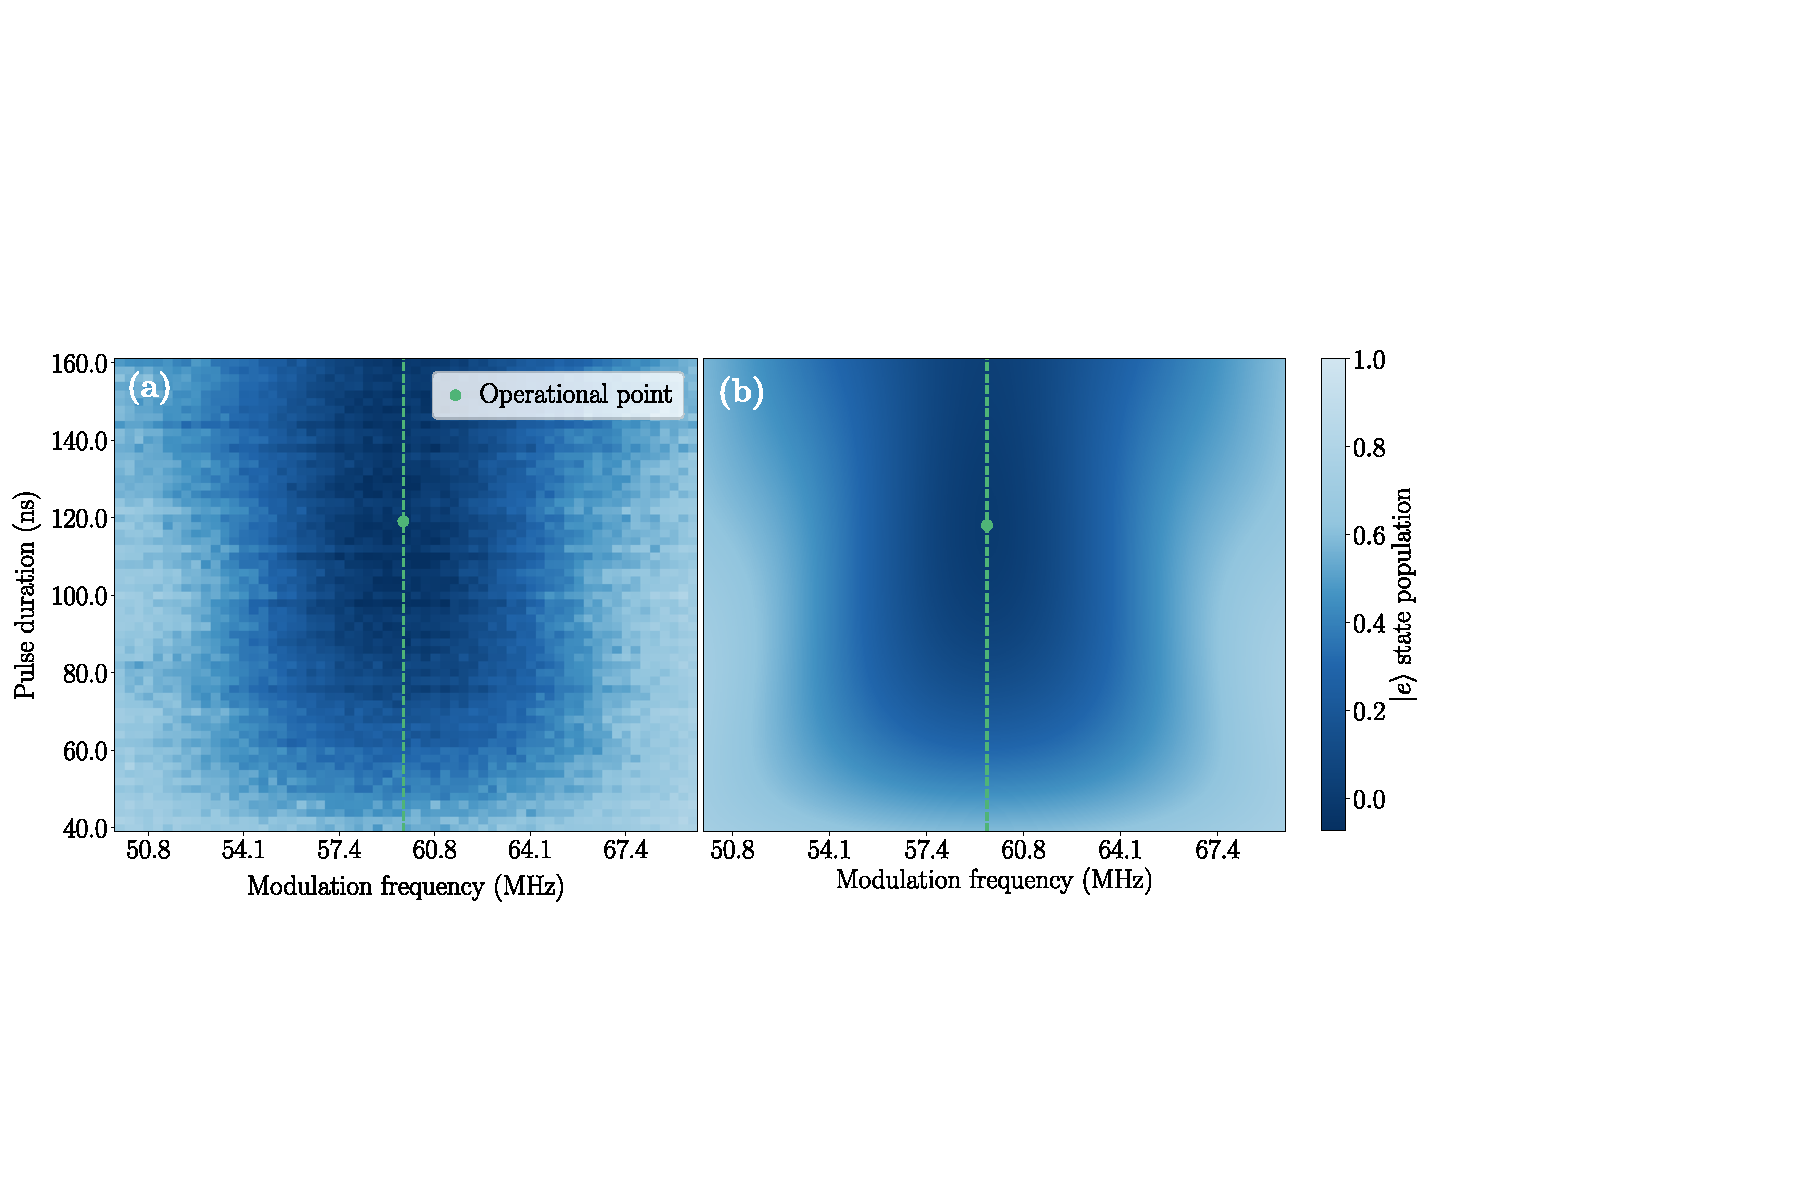
\includegraphics[width = \textwidth]{Images/Chap3/a.pdf}
    \caption{\textbf{(a)} data of the $e0g1$ transition within a storage-emitter pair with \textbf{(b)} relative fit}
    \label{fig:SWAP_chevrons}
\end{figure}

Before initiating each new protocol, it is essential to reset the population of the storage qubits.
This can be achieved through either passive waiting or by executing the resetting protocol.
Since the emitter qubit can be assured to be in the ground state, we just transfer the excitation from the storage to the respective emitter qubit, which subsequently releases them into the emission line.
In theory, achieving this could involve simply executing a SWAP gate.
However, in practice, we observe improved performance by prolonging the $e0$-$g1$ transition.
This approach achieves the desired outcome of resetting the storage qubit state to the ground state $\ket{g}$.

\subsection{CNOT}

The other operation that we can run between storage and emitter qubits is a controlled emission, or CNOT.
The unitary matrix representing this operation is
\begin{equation}
    U_{\text{CNOT}} = 
    \begin{pmatrix}
    1 & 0 & 0 & 0 \\
    0 & 1 & 0 & 0 \\
    0 & 0 & 0 & 1 \\
    0 & 0 & 1 & 0 \\
\end{pmatrix}.
\end{equation}

A photon is emitted from the emitter qubit only if the storage qubit is in the excited state $\ket{e}$, otherwise no photon is emitted.
Thus, it performs the operation
\begin{equation}
    \ket{\psi}_{\text{S}} \ket{0}_{\text{E}} = 
    (\alpha \ket{g0} + \beta \ket{e0})_{\text{SE}} \xrightarrow{U_{\text{CNOT}}}
    (\alpha \ket{g0} + \beta \ket{e1})_{\text{SE}} .
\end{equation}

Note that, since the final state cannot be expressed as a tensor product of two individual pure states, the resulting state is entangled.

\begin{figure}
    \centering
    

\tikzset{every picture/.style={line width=0.75pt}} %set default line width to 0.75pt        

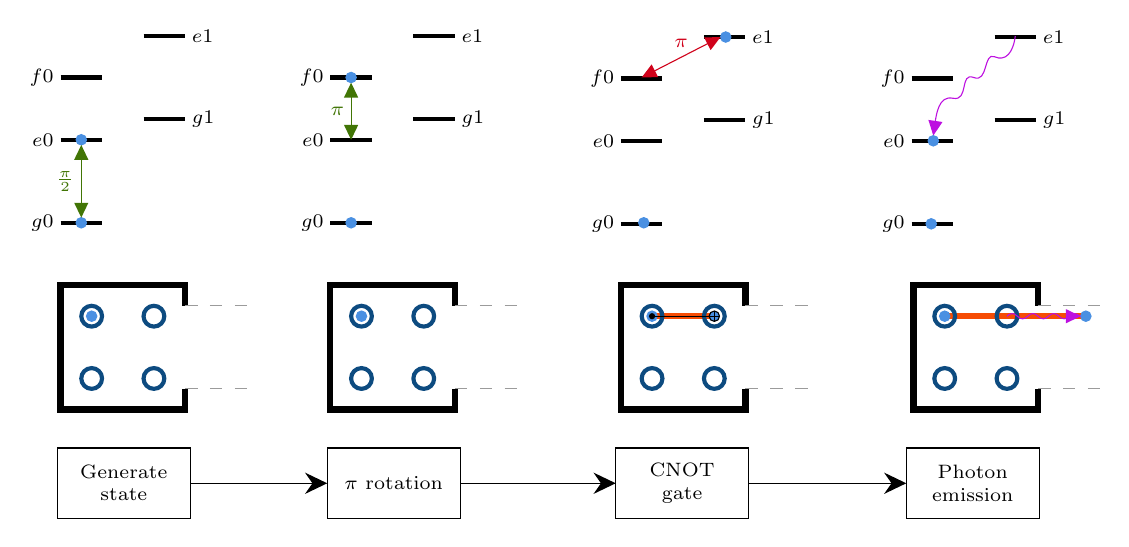
\begin{tikzpicture}[x=0.75pt,y=0.75pt,yscale=-1,xscale=1]
%uncomment if require: \path (0,369); %set diagram left start at 0, and has height of 369

%Shape: Square [id:dp16311871674784617] 
\draw  [line width=2.25]  (451,200) -- (511,200) -- (511,260) -- (451,260) -- cycle ;
%Straight Lines [id:da7729927634660387] 
\draw [color={rgb, 255:red, 255; green, 255; blue, 255 }  ,draw opacity=1 ][line width=3]    (511,210) -- (511,250) ;

%Straight Lines [id:da7800146811047701] 
\draw [color={rgb, 255:red, 246; green, 76; blue, 4 }  ,draw opacity=1 ][line width=2.25]    (466,215) -- (534,215) ;
%Straight Lines [id:da6261448047007223] 
\draw [color={rgb, 255:red, 246; green, 76; blue, 4 }  ,draw opacity=1 ][line width=2.25]    (325,215) -- (355,215) ;
%Shape: Circle [id:dp08255337848175437] 
\draw  [color={rgb, 255:red, 74; green, 144; blue, 226 }  ,draw opacity=1 ][fill={rgb, 255:red, 74; green, 144; blue, 226 }  ,fill opacity=1 ] (322.5,215) .. controls (322.5,213.62) and (323.62,212.5) .. (325,212.5) .. controls (326.38,212.5) and (327.5,213.62) .. (327.5,215) .. controls (327.5,216.38) and (326.38,217.5) .. (325,217.5) .. controls (323.62,217.5) and (322.5,216.38) .. (322.5,215) -- cycle ;
%Straight Lines [id:da9104352429816489] 
\draw [line width=1.5]    (170,100) -- (190,100) ;
%Straight Lines [id:da4044326119304753] 
\draw [line width=1.5]    (210,80) -- (230,80) ;
%Straight Lines [id:da8246098672675921] 
\draw [line width=1.5]    (170,130) -- (190,130) ;
%Straight Lines [id:da28026964700411405] 
\draw [line width=1.5]    (170,170) -- (190,170) ;
%Straight Lines [id:da6372847917499911] 
\draw [line width=1.5]    (210,120) -- (230,120) ;
%Straight Lines [id:da7158175267683015] 
\draw [line width=1.5]    (310,100.5) -- (330,100.5) ;
%Straight Lines [id:da029189986581482863] 
\draw [line width=1.5]    (350,80.5) -- (370,80.5) ;
%Straight Lines [id:da5055762916284449] 
\draw [line width=1.5]    (310,130.5) -- (330,130.5) ;
%Straight Lines [id:da12540512017651273] 
\draw [line width=1.5]    (310,170.5) -- (330,170.5) ;
%Straight Lines [id:da6841661375720638] 
\draw [line width=1.5]    (350,120.5) -- (370,120.5) ;
%Straight Lines [id:da07667408340673776] 
\draw [line width=1.5]    (450,100.5) -- (470,100.5) ;
%Straight Lines [id:da5408805406645967] 
\draw [line width=1.5]    (490,80.5) -- (510,80.5) ;
%Straight Lines [id:da29633743286868486] 
\draw [line width=1.5]    (450,130.5) -- (470,130.5) ;
%Straight Lines [id:da4224256257765836] 
\draw [line width=1.5]    (450,170.5) -- (470,170.5) ;
%Straight Lines [id:da5748015229993475] 
\draw [line width=1.5]    (490,120.5) -- (510,120.5) ;
%Shape: Circle [id:dp17205385892315683] 
\draw  [color={rgb, 255:red, 13; green, 75; blue, 128 }  ,draw opacity=1 ][line width=1.5]  (180,215) .. controls (180,212.24) and (182.24,210) .. (185,210) .. controls (187.76,210) and (190,212.24) .. (190,215) .. controls (190,217.76) and (187.76,220) .. (185,220) .. controls (182.24,220) and (180,217.76) .. (180,215) -- cycle ;
%Shape: Circle [id:dp31352659886469914] 
\draw  [color={rgb, 255:red, 13; green, 75; blue, 128 }  ,draw opacity=1 ][line width=1.5]  (180,245) .. controls (180,242.24) and (182.24,240) .. (185,240) .. controls (187.76,240) and (190,242.24) .. (190,245) .. controls (190,247.76) and (187.76,250) .. (185,250) .. controls (182.24,250) and (180,247.76) .. (180,245) -- cycle ;
%Shape: Circle [id:dp5992292171552074] 
\draw  [color={rgb, 255:red, 13; green, 75; blue, 128 }  ,draw opacity=1 ][line width=1.5]  (210,245) .. controls (210,242.24) and (212.24,240) .. (215,240) .. controls (217.76,240) and (220,242.24) .. (220,245) .. controls (220,247.76) and (217.76,250) .. (215,250) .. controls (212.24,250) and (210,247.76) .. (210,245) -- cycle ;
%Shape: Circle [id:dp5175687516944736] 
\draw  [color={rgb, 255:red, 13; green, 75; blue, 128 }  ,draw opacity=1 ][line width=1.5]  (210,215) .. controls (210,212.24) and (212.24,210) .. (215,210) .. controls (217.76,210) and (220,212.24) .. (220,215) .. controls (220,217.76) and (217.76,220) .. (215,220) .. controls (212.24,220) and (210,217.76) .. (210,215) -- cycle ;
%Shape: Square [id:dp7278738414250778] 
\draw  [line width=2.25]  (170,200) -- (230,200) -- (230,260) -- (170,260) -- cycle ;
%Straight Lines [id:da27484081993709997] 
\draw [color={rgb, 255:red, 255; green, 255; blue, 255 }  ,draw opacity=1 ][line width=3]    (230,210) -- (230,250) ;

%Shape: Circle [id:dp7417447571645056] 
\draw  [color={rgb, 255:red, 74; green, 144; blue, 226 }  ,draw opacity=1 ][fill={rgb, 255:red, 74; green, 144; blue, 226 }  ,fill opacity=1 ] (182.5,215) .. controls (182.5,213.62) and (183.62,212.5) .. (185,212.5) .. controls (186.38,212.5) and (187.5,213.62) .. (187.5,215) .. controls (187.5,216.38) and (186.38,217.5) .. (185,217.5) .. controls (183.62,217.5) and (182.5,216.38) .. (182.5,215) -- cycle ;
%Shape: Circle [id:dp5521220556000415] 
\draw  [color={rgb, 255:red, 13; green, 75; blue, 128 }  ,draw opacity=1 ][line width=1.5]  (320,215) .. controls (320,212.24) and (322.24,210) .. (325,210) .. controls (327.76,210) and (330,212.24) .. (330,215) .. controls (330,217.76) and (327.76,220) .. (325,220) .. controls (322.24,220) and (320,217.76) .. (320,215) -- cycle ;
%Shape: Circle [id:dp5119802656626787] 
\draw  [color={rgb, 255:red, 13; green, 75; blue, 128 }  ,draw opacity=1 ][line width=1.5]  (320,245) .. controls (320,242.24) and (322.24,240) .. (325,240) .. controls (327.76,240) and (330,242.24) .. (330,245) .. controls (330,247.76) and (327.76,250) .. (325,250) .. controls (322.24,250) and (320,247.76) .. (320,245) -- cycle ;
%Shape: Circle [id:dp45831332554801185] 
\draw  [color={rgb, 255:red, 13; green, 75; blue, 128 }  ,draw opacity=1 ][line width=1.5]  (350,245) .. controls (350,242.24) and (352.24,240) .. (355,240) .. controls (357.76,240) and (360,242.24) .. (360,245) .. controls (360,247.76) and (357.76,250) .. (355,250) .. controls (352.24,250) and (350,247.76) .. (350,245) -- cycle ;
%Shape: Circle [id:dp5667242703643459] 
\draw  [color={rgb, 255:red, 13; green, 75; blue, 128 }  ,draw opacity=1 ][line width=1.5]  (350,215) .. controls (350,212.24) and (352.24,210) .. (355,210) .. controls (357.76,210) and (360,212.24) .. (360,215) .. controls (360,217.76) and (357.76,220) .. (355,220) .. controls (352.24,220) and (350,217.76) .. (350,215) -- cycle ;
%Shape: Square [id:dp8519449086567641] 
\draw  [line width=2.25]  (310,200) -- (370,200) -- (370,260) -- (310,260) -- cycle ;
%Straight Lines [id:da6856000655126234] 
\draw [color={rgb, 255:red, 255; green, 255; blue, 255 }  ,draw opacity=1 ][line width=3]    (370,210) -- (370,250) ;

%Shape: Circle [id:dp20438827688260486] 
\draw  [color={rgb, 255:red, 0; green, 0; blue, 0 }  ,draw opacity=1 ][fill={rgb, 255:red, 74; green, 144; blue, 226 }  ,fill opacity=1 ] (352.5,215) .. controls (352.5,213.62) and (353.62,212.5) .. (355,212.5) .. controls (356.38,212.5) and (357.5,213.62) .. (357.5,215) .. controls (357.5,216.38) and (356.38,217.5) .. (355,217.5) .. controls (353.62,217.5) and (352.5,216.38) .. (352.5,215) -- cycle ;
%Shape: Circle [id:dp5596871069752617] 
\draw  [color={rgb, 255:red, 13; green, 75; blue, 128 }  ,draw opacity=1 ][line width=1.5]  (461,215) .. controls (461,212.24) and (463.24,210) .. (466,210) .. controls (468.76,210) and (471,212.24) .. (471,215) .. controls (471,217.76) and (468.76,220) .. (466,220) .. controls (463.24,220) and (461,217.76) .. (461,215) -- cycle ;
%Shape: Circle [id:dp23654847702851645] 
\draw  [color={rgb, 255:red, 13; green, 75; blue, 128 }  ,draw opacity=1 ][line width=1.5]  (461,245) .. controls (461,242.24) and (463.24,240) .. (466,240) .. controls (468.76,240) and (471,242.24) .. (471,245) .. controls (471,247.76) and (468.76,250) .. (466,250) .. controls (463.24,250) and (461,247.76) .. (461,245) -- cycle ;
%Shape: Circle [id:dp9337844037205707] 
\draw  [color={rgb, 255:red, 13; green, 75; blue, 128 }  ,draw opacity=1 ][line width=1.5]  (491,245) .. controls (491,242.24) and (493.24,240) .. (496,240) .. controls (498.76,240) and (501,242.24) .. (501,245) .. controls (501,247.76) and (498.76,250) .. (496,250) .. controls (493.24,250) and (491,247.76) .. (491,245) -- cycle ;
%Shape: Circle [id:dp9108295407689929] 
\draw  [color={rgb, 255:red, 13; green, 75; blue, 128 }  ,draw opacity=1 ][line width=1.5]  (491,215) .. controls (491,212.24) and (493.24,210) .. (496,210) .. controls (498.76,210) and (501,212.24) .. (501,215) .. controls (501,217.76) and (498.76,220) .. (496,220) .. controls (493.24,220) and (491,217.76) .. (491,215) -- cycle ;
%Shape: Circle [id:dp7135835004027433] 
\draw  [color={rgb, 255:red, 74; green, 144; blue, 226 }  ,draw opacity=1 ][fill={rgb, 255:red, 74; green, 144; blue, 226 }  ,fill opacity=1 ] (531.5,215) .. controls (531.5,213.62) and (532.62,212.5) .. (534,212.5) .. controls (535.38,212.5) and (536.5,213.62) .. (536.5,215) .. controls (536.5,216.38) and (535.38,217.5) .. (534,217.5) .. controls (532.62,217.5) and (531.5,216.38) .. (531.5,215) -- cycle ;
%Shape: Circle [id:dp9013057046264672] 
\draw  [color={rgb, 255:red, 74; green, 144; blue, 226 }  ,draw opacity=1 ][fill={rgb, 255:red, 74; green, 144; blue, 226 }  ,fill opacity=1 ] (177.5,170) .. controls (177.5,168.62) and (178.62,167.5) .. (180,167.5) .. controls (181.38,167.5) and (182.5,168.62) .. (182.5,170) .. controls (182.5,171.38) and (181.38,172.5) .. (180,172.5) .. controls (178.62,172.5) and (177.5,171.38) .. (177.5,170) -- cycle ;
%Shape: Circle [id:dp44633087412727634] 
\draw  [color={rgb, 255:red, 74; green, 144; blue, 226 }  ,draw opacity=1 ][fill={rgb, 255:red, 74; green, 144; blue, 226 }  ,fill opacity=1 ] (177.5,100) .. controls (177.5,98.62) and (178.62,97.5) .. (180,97.5) .. controls (181.38,97.5) and (182.5,98.62) .. (182.5,100) .. controls (182.5,101.38) and (181.38,102.5) .. (180,102.5) .. controls (178.62,102.5) and (177.5,101.38) .. (177.5,100) -- cycle ;
%Straight Lines [id:da7936001347648454] 
\draw [color={rgb, 255:red, 65; green, 117; blue, 5 }  ,draw opacity=1 ]   (180,105.5) -- (180,127) ;
\draw [shift={(180,130)}, rotate = 270] [fill={rgb, 255:red, 65; green, 117; blue, 5 }  ,fill opacity=1 ][line width=0.08]  [draw opacity=0] (7.14,-3.43) -- (0,0) -- (7.14,3.43) -- cycle    ;
\draw [shift={(180,102.5)}, rotate = 90] [fill={rgb, 255:red, 65; green, 117; blue, 5 }  ,fill opacity=1 ][line width=0.08]  [draw opacity=0] (7.14,-3.43) -- (0,0) -- (7.14,3.43) -- cycle    ;
%Shape: Circle [id:dp7488200712756418] 
\draw  [color={rgb, 255:red, 74; green, 144; blue, 226 }  ,draw opacity=1 ][fill={rgb, 255:red, 74; green, 144; blue, 226 }  ,fill opacity=1 ] (318.5,170) .. controls (318.5,168.62) and (319.62,167.5) .. (321,167.5) .. controls (322.38,167.5) and (323.5,168.62) .. (323.5,170) .. controls (323.5,171.38) and (322.38,172.5) .. (321,172.5) .. controls (319.62,172.5) and (318.5,171.38) .. (318.5,170) -- cycle ;
%Shape: Circle [id:dp5107256171224921] 
\draw  [color={rgb, 255:red, 74; green, 144; blue, 226 }  ,draw opacity=1 ][fill={rgb, 255:red, 74; green, 144; blue, 226 }  ,fill opacity=1 ] (358,80.5) .. controls (358,79.12) and (359.12,78) .. (360.5,78) .. controls (361.88,78) and (363,79.12) .. (363,80.5) .. controls (363,81.88) and (361.88,83) .. (360.5,83) .. controls (359.12,83) and (358,81.88) .. (358,80.5) -- cycle ;
%Straight Lines [id:da07777486794989807] 
\draw [color={rgb, 255:red, 208; green, 2; blue, 27 }  ,draw opacity=1 ]   (322.67,98.63) -- (355.33,81.87) ;
\draw [shift={(358,80.5)}, rotate = 152.84] [fill={rgb, 255:red, 208; green, 2; blue, 27 }  ,fill opacity=1 ][line width=0.08]  [draw opacity=0] (7.14,-3.43) -- (0,0) -- (7.14,3.43) -- cycle    ;
\draw [shift={(320,100)}, rotate = 332.84] [fill={rgb, 255:red, 208; green, 2; blue, 27 }  ,fill opacity=1 ][line width=0.08]  [draw opacity=0] (7.14,-3.43) -- (0,0) -- (7.14,3.43) -- cycle    ;
%Straight Lines [id:da706124288913454] 
\draw    (355,212.5) -- (355,218) ;
%Straight Lines [id:da8373136063677892] 
\draw    (325,215) -- (355,215) ;
%Shape: Circle [id:dp31267139017918266] 
\draw  [color={rgb, 255:red, 74; green, 144; blue, 226 }  ,draw opacity=1 ][fill={rgb, 255:red, 74; green, 144; blue, 226 }  ,fill opacity=1 ] (457,170.5) .. controls (457,169.12) and (458.12,168) .. (459.5,168) .. controls (460.88,168) and (462,169.12) .. (462,170.5) .. controls (462,171.88) and (460.88,173) .. (459.5,173) .. controls (458.12,173) and (457,171.88) .. (457,170.5) -- cycle ;
%Curve Lines [id:da857229348858473] 
\draw [color={rgb, 255:red, 189; green, 16; blue, 224 }  ,draw opacity=1 ]   (500,80) .. controls (499,88) and (495.4,92.4) .. (490,90) .. controls (484.6,87.6) and (487,102.8) .. (480,100) .. controls (473,97.2) and (477.8,111.6) .. (470,110) .. controls (463.06,108.58) and (461.94,117.11) .. (460.89,125.09) ;
\draw [shift={(460.5,128)}, rotate = 278.25] [fill={rgb, 255:red, 189; green, 16; blue, 224 }  ,fill opacity=1 ][line width=0.08]  [draw opacity=0] (7.14,-3.43) -- (0,0) -- (7.14,3.43) -- cycle    ;
%Straight Lines [id:da889905748540048] 
\draw [color={rgb, 255:red, 155; green, 155; blue, 155 }  ,draw opacity=1 ] [dash pattern={on 4.5pt off 4.5pt}]  (230,210) -- (260,210) ;
%Straight Lines [id:da16372018131925703] 
\draw [color={rgb, 255:red, 189; green, 16; blue, 224 }  ,draw opacity=1 ]   (496,215) .. controls (497.67,213.33) and (499.33,213.33) .. (501,215) .. controls (502.67,216.67) and (504.33,216.67) .. (506,215) .. controls (507.67,213.33) and (509.33,213.33) .. (511,215) .. controls (512.67,216.67) and (514.33,216.67) .. (516,215) .. controls (517.67,213.33) and (519.33,213.33) .. (521,215) .. controls (522.67,216.67) and (524.33,216.67) .. (526,215) .. controls (527.67,213.33) and (529.33,213.33) .. (531,215) -- (531.5,215) -- (531.5,215) ;
%Straight Lines [id:da2997477939659331] 
\draw [color={rgb, 255:red, 155; green, 155; blue, 155 }  ,draw opacity=1 ] [dash pattern={on 4.5pt off 4.5pt}]  (230,250) -- (260,250) ;
%Straight Lines [id:da5918955553719868] 
\draw [color={rgb, 255:red, 155; green, 155; blue, 155 }  ,draw opacity=1 ] [dash pattern={on 4.5pt off 4.5pt}]  (511,210) -- (541,210) ;
%Straight Lines [id:da0486299340629458] 
\draw [color={rgb, 255:red, 155; green, 155; blue, 155 }  ,draw opacity=1 ] [dash pattern={on 4.5pt off 4.5pt}]  (511,250) -- (541,250) ;
%Straight Lines [id:da9343610277610461] 
\draw [color={rgb, 255:red, 155; green, 155; blue, 155 }  ,draw opacity=1 ] [dash pattern={on 4.5pt off 4.5pt}]  (370,210) -- (400,210) ;
%Straight Lines [id:da9867104981357256] 
\draw [color={rgb, 255:red, 155; green, 155; blue, 155 }  ,draw opacity=1 ] [dash pattern={on 4.5pt off 4.5pt}]  (370,250) -- (400,250) ;
%Straight Lines [id:da8263464719156766] 
\draw [color={rgb, 255:red, 189; green, 16; blue, 224 }  ,draw opacity=1 ]   (525.75,215) -- (528.5,215) ;
\draw [shift={(531.5,215)}, rotate = 180] [fill={rgb, 255:red, 189; green, 16; blue, 224 }  ,fill opacity=1 ][line width=0.08]  [draw opacity=0] (7.14,-3.43) -- (0,0) -- (7.14,3.43) -- cycle    ;
%Straight Lines [id:da9996253266141027] 
\draw [line width=1.5]    (40,100) -- (60,100) ;
%Straight Lines [id:da008787592451602766] 
\draw [line width=1.5]    (80,80) -- (100,80) ;
%Straight Lines [id:da01542378337792405] 
\draw [line width=1.5]    (40,130) -- (60,130) ;
%Straight Lines [id:da5801688716124229] 
\draw [line width=1.5]    (40,170) -- (60,170) ;
%Straight Lines [id:da7416093809083778] 
\draw [line width=1.5]    (80,120) -- (100,120) ;
%Shape: Circle [id:dp40133823415950687] 
\draw  [color={rgb, 255:red, 13; green, 75; blue, 128 }  ,draw opacity=1 ][line width=1.5]  (50,215) .. controls (50,212.24) and (52.24,210) .. (55,210) .. controls (57.76,210) and (60,212.24) .. (60,215) .. controls (60,217.76) and (57.76,220) .. (55,220) .. controls (52.24,220) and (50,217.76) .. (50,215) -- cycle ;
%Shape: Circle [id:dp5122255712488911] 
\draw  [color={rgb, 255:red, 13; green, 75; blue, 128 }  ,draw opacity=1 ][line width=1.5]  (50,245) .. controls (50,242.24) and (52.24,240) .. (55,240) .. controls (57.76,240) and (60,242.24) .. (60,245) .. controls (60,247.76) and (57.76,250) .. (55,250) .. controls (52.24,250) and (50,247.76) .. (50,245) -- cycle ;
%Shape: Circle [id:dp22665586503294544] 
\draw  [color={rgb, 255:red, 13; green, 75; blue, 128 }  ,draw opacity=1 ][line width=1.5]  (80,245) .. controls (80,242.24) and (82.24,240) .. (85,240) .. controls (87.76,240) and (90,242.24) .. (90,245) .. controls (90,247.76) and (87.76,250) .. (85,250) .. controls (82.24,250) and (80,247.76) .. (80,245) -- cycle ;
%Shape: Circle [id:dp2180155808041916] 
\draw  [color={rgb, 255:red, 13; green, 75; blue, 128 }  ,draw opacity=1 ][line width=1.5]  (80,215) .. controls (80,212.24) and (82.24,210) .. (85,210) .. controls (87.76,210) and (90,212.24) .. (90,215) .. controls (90,217.76) and (87.76,220) .. (85,220) .. controls (82.24,220) and (80,217.76) .. (80,215) -- cycle ;
%Shape: Square [id:dp2787436056127518] 
\draw  [line width=2.25]  (40,200) -- (100,200) -- (100,260) -- (40,260) -- cycle ;
%Straight Lines [id:da045371293369983134] 
\draw [color={rgb, 255:red, 255; green, 255; blue, 255 }  ,draw opacity=1 ][line width=3]    (100,210) -- (100,250) ;

%Shape: Circle [id:dp6587846640355887] 
\draw  [color={rgb, 255:red, 74; green, 144; blue, 226 }  ,draw opacity=1 ][fill={rgb, 255:red, 74; green, 144; blue, 226 }  ,fill opacity=1 ] (52.5,215) .. controls (52.5,213.62) and (53.62,212.5) .. (55,212.5) .. controls (56.38,212.5) and (57.5,213.62) .. (57.5,215) .. controls (57.5,216.38) and (56.38,217.5) .. (55,217.5) .. controls (53.62,217.5) and (52.5,216.38) .. (52.5,215) -- cycle ;
%Shape: Circle [id:dp6256247076231964] 
\draw  [color={rgb, 255:red, 74; green, 144; blue, 226 }  ,draw opacity=1 ][fill={rgb, 255:red, 74; green, 144; blue, 226 }  ,fill opacity=1 ] (47.5,170) .. controls (47.5,168.62) and (48.62,167.5) .. (50,167.5) .. controls (51.38,167.5) and (52.5,168.62) .. (52.5,170) .. controls (52.5,171.38) and (51.38,172.5) .. (50,172.5) .. controls (48.62,172.5) and (47.5,171.38) .. (47.5,170) -- cycle ;
%Shape: Circle [id:dp01199037432900818] 
\draw  [color={rgb, 255:red, 74; green, 144; blue, 226 }  ,draw opacity=1 ][fill={rgb, 255:red, 74; green, 144; blue, 226 }  ,fill opacity=1 ] (47.5,130) .. controls (47.5,128.62) and (48.62,127.5) .. (50,127.5) .. controls (51.38,127.5) and (52.5,128.62) .. (52.5,130) .. controls (52.5,131.38) and (51.38,132.5) .. (50,132.5) .. controls (48.62,132.5) and (47.5,131.38) .. (47.5,130) -- cycle ;
%Straight Lines [id:da9386095793305913] 
\draw [color={rgb, 255:red, 65; green, 117; blue, 5 }  ,draw opacity=1 ]   (50,135.5) -- (50,164.5) ;
\draw [shift={(50,167.5)}, rotate = 270] [fill={rgb, 255:red, 65; green, 117; blue, 5 }  ,fill opacity=1 ][line width=0.08]  [draw opacity=0] (7.14,-3.43) -- (0,0) -- (7.14,3.43) -- cycle    ;
\draw [shift={(50,132.5)}, rotate = 90] [fill={rgb, 255:red, 65; green, 117; blue, 5 }  ,fill opacity=1 ][line width=0.08]  [draw opacity=0] (7.14,-3.43) -- (0,0) -- (7.14,3.43) -- cycle    ;
%Straight Lines [id:da5020447437638056] 
\draw [color={rgb, 255:red, 155; green, 155; blue, 155 }  ,draw opacity=1 ] [dash pattern={on 4.5pt off 4.5pt}]  (100,210) -- (130,210) ;
%Straight Lines [id:da7360195994256211] 
\draw [color={rgb, 255:red, 155; green, 155; blue, 155 }  ,draw opacity=1 ] [dash pattern={on 4.5pt off 4.5pt}]  (100,250) -- (130,250) ;
%Shape: Circle [id:dp13852193266636725] 
\draw  [color={rgb, 255:red, 74; green, 144; blue, 226 }  ,draw opacity=1 ][fill={rgb, 255:red, 74; green, 144; blue, 226 }  ,fill opacity=1 ] (458,130.5) .. controls (458,129.12) and (459.12,128) .. (460.5,128) .. controls (461.88,128) and (463,129.12) .. (463,130.5) .. controls (463,131.88) and (461.88,133) .. (460.5,133) .. controls (459.12,133) and (458,131.88) .. (458,130.5) -- cycle ;
%Straight Lines [id:da6688912999251266] 
\draw    (357.5,215) -- (352.5,215) ;
%Shape: Circle [id:dp8863197645267697] 
\draw  [draw opacity=0][fill={rgb, 255:red, 0; green, 0; blue, 0 }  ,fill opacity=1 ] (323.5,215) .. controls (323.5,214.17) and (324.17,213.5) .. (325,213.5) .. controls (325.83,213.5) and (326.5,214.17) .. (326.5,215) .. controls (326.5,215.83) and (325.83,216.5) .. (325,216.5) .. controls (324.17,216.5) and (323.5,215.83) .. (323.5,215) -- cycle ;
%Shape: Circle [id:dp0025570249322276473] 
\draw  [color={rgb, 255:red, 74; green, 144; blue, 226 }  ,draw opacity=1 ][fill={rgb, 255:red, 74; green, 144; blue, 226 }  ,fill opacity=1 ] (463.5,215) .. controls (463.5,213.62) and (464.62,212.5) .. (466,212.5) .. controls (467.38,212.5) and (468.5,213.62) .. (468.5,215) .. controls (468.5,216.38) and (467.38,217.5) .. (466,217.5) .. controls (464.62,217.5) and (463.5,216.38) .. (463.5,215) -- cycle ;

% Text Node
\draw (168,100) node [anchor=east] [inner sep=0.75pt]  [font=\scriptsize]  {$f0$};
% Text Node
\draw (168,130) node [anchor=east] [inner sep=0.75pt]  [font=\scriptsize]  {$e0$};
% Text Node
\draw (168,170) node [anchor=east] [inner sep=0.75pt]  [font=\scriptsize]  {$g0$};
% Text Node
\draw (232,80) node [anchor=west] [inner sep=0.75pt]  [font=\scriptsize]  {$e1$};
% Text Node
\draw (232,120) node [anchor=west] [inner sep=0.75pt]  [font=\scriptsize]  {$g1$};
% Text Node
\draw (308,100.5) node [anchor=east] [inner sep=0.75pt]  [font=\scriptsize]  {$f0$};
% Text Node
\draw (308,130.5) node [anchor=east] [inner sep=0.75pt]  [font=\scriptsize]  {$e0$};
% Text Node
\draw (308,170.5) node [anchor=east] [inner sep=0.75pt]  [font=\scriptsize]  {$g0$};
% Text Node
\draw (372,80.5) node [anchor=west] [inner sep=0.75pt]  [font=\scriptsize]  {$e1$};
% Text Node
\draw (372,120.5) node [anchor=west] [inner sep=0.75pt]  [font=\scriptsize]  {$g1$};
% Text Node
\draw (448,100.5) node [anchor=east] [inner sep=0.75pt]  [font=\scriptsize]  {$f0$};
% Text Node
\draw (448,130.5) node [anchor=east] [inner sep=0.75pt]  [font=\scriptsize]  {$e0$};
% Text Node
\draw (448,170.5) node [anchor=east] [inner sep=0.75pt]  [font=\scriptsize]  {$g0$};
% Text Node
\draw (512,80.5) node [anchor=west] [inner sep=0.75pt]  [font=\scriptsize]  {$e1$};
% Text Node
\draw (512,120.5) node [anchor=west] [inner sep=0.75pt]  [font=\scriptsize]  {$g1$};
% Text Node
\draw (178,116.25) node [anchor=east] [inner sep=0.75pt]  [font=\scriptsize,color={rgb, 255:red, 65; green, 117; blue, 5 }  ,opacity=1 ]  {$\pi $};
% Text Node
\draw (339,86.85) node [anchor=south] [inner sep=0.75pt]  [font=\scriptsize,color={rgb, 255:red, 208; green, 2; blue, 27 }  ,opacity=1 ]  {$\pi $};
% Text Node
\draw    (168.5,278.5) -- (232.5,278.5) -- (232.5,312.5) -- (168.5,312.5) -- cycle  ;
\draw (200.5,295.5) node  [font=\scriptsize] [align=left] {\begin{minipage}[lt]{40.8pt}\setlength\topsep{0pt}
\begin{center}
$\displaystyle \pi $ rotation
\end{center}

\end{minipage}};
% Text Node
\draw    (307.5,278.5) -- (371.5,278.5) -- (371.5,312.5) -- (307.5,312.5) -- cycle  ;
\draw (339.5,295.5) node  [font=\scriptsize] [align=left] {\begin{minipage}[lt]{40.8pt}\setlength\topsep{0pt}
\begin{center}
CNOT\\gate
\end{center}

\end{minipage}};
% Text Node
\draw    (447.5,278.5) -- (511.5,278.5) -- (511.5,312.5) -- (447.5,312.5) -- cycle  ;
\draw (479.5,295.5) node  [font=\scriptsize] [align=left] {\begin{minipage}[lt]{40.8pt}\setlength\topsep{0pt}
\begin{center}
Photon\\emission
\end{center}

\end{minipage}};
% Text Node
\draw (38,100) node [anchor=east] [inner sep=0.75pt]  [font=\scriptsize]  {$f0$};
% Text Node
\draw (38,130) node [anchor=east] [inner sep=0.75pt]  [font=\scriptsize]  {$e0$};
% Text Node
\draw (38,170) node [anchor=east] [inner sep=0.75pt]  [font=\scriptsize]  {$g0$};
% Text Node
\draw (102,80) node [anchor=west] [inner sep=0.75pt]  [font=\scriptsize]  {$e1$};
% Text Node
\draw (102,120) node [anchor=west] [inner sep=0.75pt]  [font=\scriptsize]  {$g1$};
% Text Node
\draw (48,150) node [anchor=east] [inner sep=0.75pt]  [font=\scriptsize,color={rgb, 255:red, 65; green, 117; blue, 5 }  ,opacity=1 ]  {$\frac{\pi}{2}$};
% Text Node
\draw    (38.5,278.5) -- (102.5,278.5) -- (102.5,312.5) -- (38.5,312.5) -- cycle  ;
\draw (70.5,295.5) node  [font=\scriptsize] [align=left] {\begin{minipage}[lt]{40.8pt}\setlength\topsep{0pt}
\begin{center}
Generate state
\end{center}

\end{minipage}};
% Connection
\draw    (232.5,295.5) -- (304.5,295.5) ;
\draw [shift={(307.5,295.5)}, rotate = 180] [fill={rgb, 255:red, 0; green, 0; blue, 0 }  ][line width=0.08]  [draw opacity=0] (10.72,-5.15) -- (0,0) -- (10.72,5.15) -- (7.12,0) -- cycle    ;
% Connection
\draw    (371.5,295.5) -- (444.5,295.5) ;
\draw [shift={(447.5,295.5)}, rotate = 180] [fill={rgb, 255:red, 0; green, 0; blue, 0 }  ][line width=0.08]  [draw opacity=0] (10.72,-5.15) -- (0,0) -- (10.72,5.15) -- (7.12,0) -- cycle    ;
% Connection
\draw    (102.5,295.5) -- (165.5,295.5) ;
\draw [shift={(168.5,295.5)}, rotate = 180] [fill={rgb, 255:red, 0; green, 0; blue, 0 }  ][line width=0.08]  [draw opacity=0] (10.72,-5.15) -- (0,0) -- (10.72,5.15) -- (7.12,0) -- cycle    ;

\end{tikzpicture}
    \vspace{-1cm}
    \caption{Protocol for S-E CNOT gate}
    \label{fig:SE_CNOT}
\end{figure}

Due to the strong coupling between the emitter and the emission line, we cannot depend on operations that involve transferring population to the emitter qubit and its subsequent return.
Essentially, our capability allows only for a $\pi$ rotation between the storage and emitter qubits.
Hence, to execute a CNOT gate within our protocol, the initial step involves population transfer from the $e0$ to the $f0$ state through a single-qubit $\pi$ rotation. 
Subsequently, a $\pi$ rotation within the $f0$-$e1$ manifold is performed, effectively transferring the state from the $e0$ level to the $e1$ level within the two-qubit system.

The protocol employed for executing the controlled emission is depicted in \cref{fig:SE_CNOT}.
Within the diagram, the entanglement between the two qubits is denoted by a red line. We will discuss what we mean by entanglement when dealing with graph states in \cref{Chap:graph_states}.
It is important to highlight that, for consistency between this section and \cref{Chap:graph_states}, the state produced in the initial step is not arbitrary, but rather a $\ket{+}$ state.
This precaution arises from the meaning of the red bonds shown in the diagram, which carry specific implications within graph states, as long as the blue circles symbolize $\ket{+}$ states.

Please note, this method effectively executes a CNOT gate within the S-E manifold, operating under the assumption that the emitter qubit is in its ground state $\ket{0}$.

Similar to the protocol involved in implementing the SWAP gate, the realization of the CNOT gate also involves an operation that switches on the interaction between the two qubits. 
We calibrate this interaction in a similar way to the previous procedure, using \cref{eq:chevron_kappa}  in order to find the operational point, given by \cref{eq:tilde_t_kappa}.
Some data taken for this purpose together with optimal operational point is shown in \cref{fig:CNOT_data}.
Notice that the difference with \cref{fig:SWAP_chevrons} is that now the $\ket{f}$ population is shown.

\begin{figure}
    \centering
    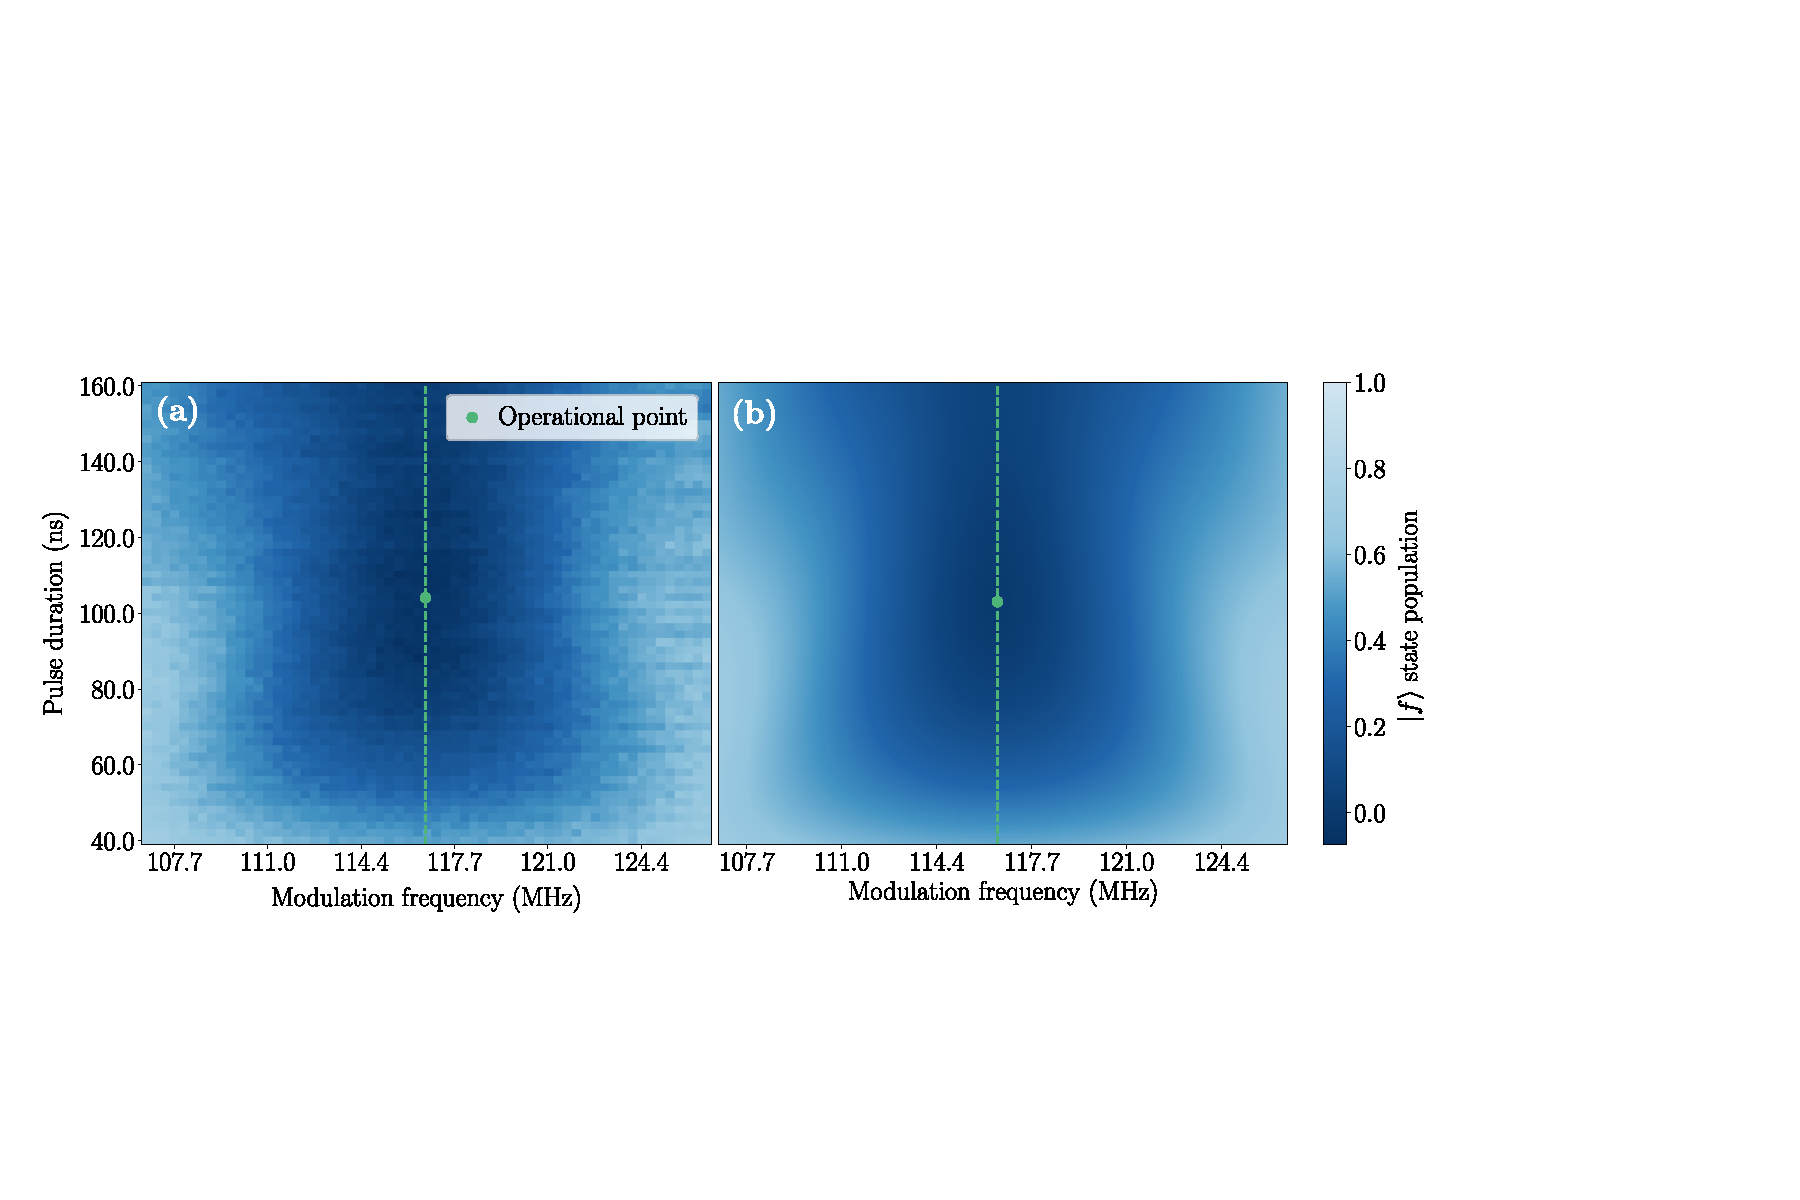
\includegraphics[width = \textwidth]{Images/Chap3/a_2.pdf}
    \caption{\textbf{(a)} data of the $f0e1$ transition within a storage-emitter pair with \textbf{(b)} relative fit}
    \label{fig:CNOT_data}
\end{figure}


\section{Storage-Storage}
\label{sec:S-S}

In the Storage-Storage system (S-S), the extended lifetime of the two qubits allows us to execute single-qubit gates on them.
Additionally, the capability to perform $2\pi$ rotations on the sidebands of this two-qubit system enables the implementation of a CZ gate within the S-S system.

\begin{figure}[b]
    \centering
    

\tikzset{every picture/.style={line width=0.75pt}} %set default line width to 0.75pt        

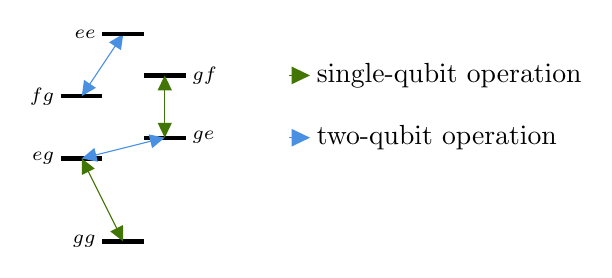
\begin{tikzpicture}[x=0.75pt,y=0.75pt,yscale=-1,xscale=1]
%uncomment if require: \path (0,300); %set diagram left start at 0, and has height of 300

%Straight Lines [id:da9559663622579351] 
\draw [line width=1.5]    (100,100) -- (120,100) ;
%Straight Lines [id:da38130444644691297] 
\draw [line width=1.5]    (140,90) -- (160,90) ;
%Straight Lines [id:da2359488638530448] 
\draw [line width=1.5]    (100,130) -- (120,130) ;
%Straight Lines [id:da3841009239924672] 
\draw [line width=1.5]    (120,170) -- (140,170) ;
%Straight Lines [id:da5788606590900368] 
\draw [line width=1.5]    (140,120) -- (160,120) ;
%Straight Lines [id:da9477773949836692] 
\draw [color={rgb, 255:red, 65; green, 117; blue, 5 }  ,draw opacity=1 ]   (111.34,132.68) -- (128.66,167.32) ;
\draw [shift={(130,170)}, rotate = 243.43] [fill={rgb, 255:red, 65; green, 117; blue, 5 }  ,fill opacity=1 ][line width=0.08]  [draw opacity=0] (7.14,-3.43) -- (0,0) -- (7.14,3.43) -- cycle    ;
\draw [shift={(110,130)}, rotate = 63.43] [fill={rgb, 255:red, 65; green, 117; blue, 5 }  ,fill opacity=1 ][line width=0.08]  [draw opacity=0] (7.14,-3.43) -- (0,0) -- (7.14,3.43) -- cycle    ;
%Straight Lines [id:da6539701699881647] 
\draw [color={rgb, 255:red, 74; green, 144; blue, 226 }  ,draw opacity=1 ]   (128.34,72.5) -- (111.66,97.5) ;
\draw [shift={(110,100)}, rotate = 303.69] [fill={rgb, 255:red, 74; green, 144; blue, 226 }  ,fill opacity=1 ][line width=0.08]  [draw opacity=0] (7.14,-3.43) -- (0,0) -- (7.14,3.43) -- cycle    ;
\draw [shift={(130,70)}, rotate = 123.69] [fill={rgb, 255:red, 74; green, 144; blue, 226 }  ,fill opacity=1 ][line width=0.08]  [draw opacity=0] (7.14,-3.43) -- (0,0) -- (7.14,3.43) -- cycle    ;
%Straight Lines [id:da6430626577491835] 
\draw [color={rgb, 255:red, 65; green, 117; blue, 5 }  ,draw opacity=1 ]   (210,90) -- (217,90) ;
\draw [shift={(220,90)}, rotate = 180] [fill={rgb, 255:red, 65; green, 117; blue, 5 }  ,fill opacity=1 ][line width=0.08]  [draw opacity=0] (8.93,-4.29) -- (0,0) -- (8.93,4.29) -- cycle    ;
%Straight Lines [id:da593444231277527] 
\draw [color={rgb, 255:red, 74; green, 144; blue, 226 }  ,draw opacity=1 ]   (210,120) -- (217,120) ;
\draw [shift={(220,120)}, rotate = 180] [fill={rgb, 255:red, 74; green, 144; blue, 226 }  ,fill opacity=1 ][line width=0.08]  [draw opacity=0] (8.93,-4.29) -- (0,0) -- (8.93,4.29) -- cycle    ;
%Straight Lines [id:da04551771823475548] 
\draw [line width=1.5]    (120,70) -- (140,70) ;
%Straight Lines [id:da8060801042251682] 
\draw [color={rgb, 255:red, 65; green, 117; blue, 5 }  ,draw opacity=1 ]   (150,93) -- (150,117) ;
\draw [shift={(150,120)}, rotate = 270] [fill={rgb, 255:red, 65; green, 117; blue, 5 }  ,fill opacity=1 ][line width=0.08]  [draw opacity=0] (7.14,-3.43) -- (0,0) -- (7.14,3.43) -- cycle    ;
\draw [shift={(150,90)}, rotate = 90] [fill={rgb, 255:red, 65; green, 117; blue, 5 }  ,fill opacity=1 ][line width=0.08]  [draw opacity=0] (7.14,-3.43) -- (0,0) -- (7.14,3.43) -- cycle    ;
%Straight Lines [id:da40683969551339827] 
\draw [color={rgb, 255:red, 74; green, 144; blue, 226 }  ,draw opacity=1 ]   (112.91,129.27) -- (147.09,120.73) ;
\draw [shift={(150,120)}, rotate = 165.96] [fill={rgb, 255:red, 74; green, 144; blue, 226 }  ,fill opacity=1 ][line width=0.08]  [draw opacity=0] (7.14,-3.43) -- (0,0) -- (7.14,3.43) -- cycle    ;
\draw [shift={(110,130)}, rotate = 345.96] [fill={rgb, 255:red, 74; green, 144; blue, 226 }  ,fill opacity=1 ][line width=0.08]  [draw opacity=0] (7.14,-3.43) -- (0,0) -- (7.14,3.43) -- cycle    ;

% Text Node
\draw (98,100) node [anchor=east] [inner sep=0.75pt]  [font=\scriptsize]  {$fg$};
% Text Node
\draw (98,130) node [anchor=east] [inner sep=0.75pt]  [font=\scriptsize]  {$eg$};
% Text Node
\draw (118,170) node [anchor=east] [inner sep=0.75pt]  [font=\scriptsize]  {$gg$};
% Text Node
\draw (162,90) node [anchor=west] [inner sep=0.75pt]  [font=\scriptsize]  {$gf$};
% Text Node
\draw (162,120) node [anchor=west] [inner sep=0.75pt]  [font=\scriptsize]  {$ge$};
% Text Node
\draw (222,90) node [anchor=west] [inner sep=0.75pt]   [align=left] {single-qubit operation};
% Text Node
\draw (222,120) node [anchor=west] [inner sep=0.75pt]   [align=left] {two-qubit operation};
% Text Node
\draw (118,70) node [anchor=east] [inner sep=0.75pt]  [font=\scriptsize]  {$ee$};


\end{tikzpicture}
    \vspace{-1cm}
    \caption{Level diagram of storage-storage interaction}
    \label{fig:SS_level}
\end{figure}

In \cref{fig:SS_level}, the energy levels of the two-qubits system is shown, together with some single- and two-qubit gates that we can run on them.

\subsection{CZ}

The unitary matrix representing a controlled-phase gate, or CZ, is
\begin{equation}
    U_{\text{CZ}} = 
    \begin{pmatrix}
    1 & 0 & 0 & 0 \\
    0 & 1 & 0 & 0 \\
    0 & 0 & 1 & 0 \\
    0 & 0 & 0 & -1 \\
\end{pmatrix}.
\end{equation}

It performs the operation
\begin{equation}
    (\alpha \ket{gg} + \beta \ket{ge} + \gamma \ket{eg} + \delta \ket{ee})_{\text{S}_1 \text{S}_2} \xrightarrow{U_{\text{CZ}}}
    (\alpha \ket{gg} + \beta \ket{ge} + \gamma \ket{eg} - \delta \ket{ee})_{\text{S}_1 \text{S}_2} . 
\end{equation}

The operational sequence on our device involves transferring population between the states $\ket{ee}$ and $\ket{fg}$ within the S-S system.
After a $2\pi$ rotation, the population returns to the $\ket{ee}$ state, but with an opposite phase (see \cref{fig:SS_CZ}), effectively implementing a CZ gate.

\begin{figure}
    \centering
    

\tikzset{every picture/.style={line width=0.75pt}} %set default line width to 0.75pt        

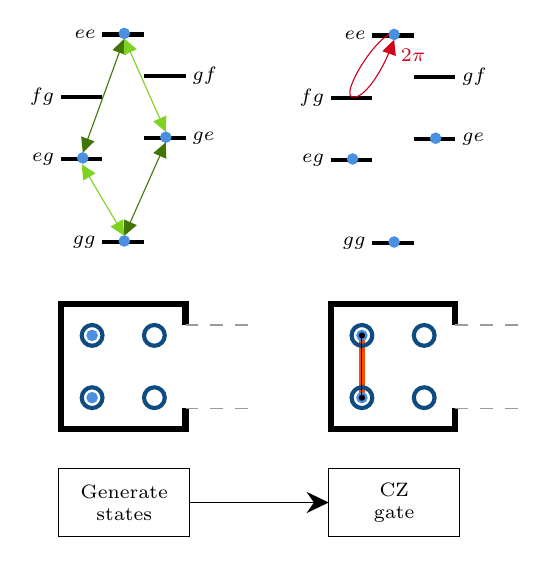
\begin{tikzpicture}[x=0.75pt,y=0.75pt,yscale=-1,xscale=1]
%uncomment if require: \path (0,369); %set diagram left start at 0, and has height of 369

%Straight Lines [id:da14238319538466393] 
\draw [color={rgb, 255:red, 246; green, 76; blue, 4 }  ,draw opacity=1 ][line width=2.25]    (185,215) -- (185,245) ;
%Shape: Circle [id:dp6131452055369363] 
\draw  [color={rgb, 255:red, 13; green, 75; blue, 128 }  ,draw opacity=1 ][line width=1.5]  (180,215) .. controls (180,212.24) and (182.24,210) .. (185,210) .. controls (187.76,210) and (190,212.24) .. (190,215) .. controls (190,217.76) and (187.76,220) .. (185,220) .. controls (182.24,220) and (180,217.76) .. (180,215) -- cycle ;
%Shape: Circle [id:dp044196496820445685] 
\draw  [color={rgb, 255:red, 13; green, 75; blue, 128 }  ,draw opacity=1 ][line width=1.5]  (180,245) .. controls (180,242.24) and (182.24,240) .. (185,240) .. controls (187.76,240) and (190,242.24) .. (190,245) .. controls (190,247.76) and (187.76,250) .. (185,250) .. controls (182.24,250) and (180,247.76) .. (180,245) -- cycle ;
%Shape: Circle [id:dp5885154746260259] 
\draw  [color={rgb, 255:red, 13; green, 75; blue, 128 }  ,draw opacity=1 ][line width=1.5]  (210,245) .. controls (210,242.24) and (212.24,240) .. (215,240) .. controls (217.76,240) and (220,242.24) .. (220,245) .. controls (220,247.76) and (217.76,250) .. (215,250) .. controls (212.24,250) and (210,247.76) .. (210,245) -- cycle ;
%Shape: Circle [id:dp7469388514126467] 
\draw  [color={rgb, 255:red, 13; green, 75; blue, 128 }  ,draw opacity=1 ][line width=1.5]  (210,215) .. controls (210,212.24) and (212.24,210) .. (215,210) .. controls (217.76,210) and (220,212.24) .. (220,215) .. controls (220,217.76) and (217.76,220) .. (215,220) .. controls (212.24,220) and (210,217.76) .. (210,215) -- cycle ;
%Shape: Square [id:dp8509793592974496] 
\draw  [line width=2.25]  (170,200) -- (230,200) -- (230,260) -- (170,260) -- cycle ;
%Straight Lines [id:da12483962352096123] 
\draw [color={rgb, 255:red, 255; green, 255; blue, 255 }  ,draw opacity=1 ][line width=3]    (230,210) -- (230,250) ;

%Shape: Circle [id:dp2946136793659927] 
\draw  [color={rgb, 255:red, 74; green, 144; blue, 226 }  ,draw opacity=1 ][fill={rgb, 255:red, 74; green, 144; blue, 226 }  ,fill opacity=1 ] (182.5,215) .. controls (182.5,213.62) and (183.62,212.5) .. (185,212.5) .. controls (186.38,212.5) and (187.5,213.62) .. (187.5,215) .. controls (187.5,216.38) and (186.38,217.5) .. (185,217.5) .. controls (183.62,217.5) and (182.5,216.38) .. (182.5,215) -- cycle ;
%Straight Lines [id:da5174133920036248] 
\draw [color={rgb, 255:red, 155; green, 155; blue, 155 }  ,draw opacity=1 ] [dash pattern={on 4.5pt off 4.5pt}]  (230,210) -- (260,210) ;
%Straight Lines [id:da26746057224200814] 
\draw [color={rgb, 255:red, 155; green, 155; blue, 155 }  ,draw opacity=1 ] [dash pattern={on 4.5pt off 4.5pt}]  (230,250) -- (260,250) ;
%Shape: Circle [id:dp9726522957124347] 
\draw  [color={rgb, 255:red, 13; green, 75; blue, 128 }  ,draw opacity=1 ][line width=1.5]  (50,215) .. controls (50,212.24) and (52.24,210) .. (55,210) .. controls (57.76,210) and (60,212.24) .. (60,215) .. controls (60,217.76) and (57.76,220) .. (55,220) .. controls (52.24,220) and (50,217.76) .. (50,215) -- cycle ;
%Shape: Circle [id:dp5051693054900083] 
\draw  [color={rgb, 255:red, 13; green, 75; blue, 128 }  ,draw opacity=1 ][line width=1.5]  (50,245) .. controls (50,242.24) and (52.24,240) .. (55,240) .. controls (57.76,240) and (60,242.24) .. (60,245) .. controls (60,247.76) and (57.76,250) .. (55,250) .. controls (52.24,250) and (50,247.76) .. (50,245) -- cycle ;
%Shape: Circle [id:dp6033756962982088] 
\draw  [color={rgb, 255:red, 13; green, 75; blue, 128 }  ,draw opacity=1 ][line width=1.5]  (80,245) .. controls (80,242.24) and (82.24,240) .. (85,240) .. controls (87.76,240) and (90,242.24) .. (90,245) .. controls (90,247.76) and (87.76,250) .. (85,250) .. controls (82.24,250) and (80,247.76) .. (80,245) -- cycle ;
%Shape: Circle [id:dp651180579558279] 
\draw  [color={rgb, 255:red, 13; green, 75; blue, 128 }  ,draw opacity=1 ][line width=1.5]  (80,215) .. controls (80,212.24) and (82.24,210) .. (85,210) .. controls (87.76,210) and (90,212.24) .. (90,215) .. controls (90,217.76) and (87.76,220) .. (85,220) .. controls (82.24,220) and (80,217.76) .. (80,215) -- cycle ;
%Shape: Square [id:dp8220576054517261] 
\draw  [line width=2.25]  (40,200) -- (100,200) -- (100,260) -- (40,260) -- cycle ;
%Straight Lines [id:da3250679662921139] 
\draw [color={rgb, 255:red, 255; green, 255; blue, 255 }  ,draw opacity=1 ][line width=3]    (100,210) -- (100,250) ;

%Shape: Circle [id:dp1764454757841779] 
\draw  [color={rgb, 255:red, 74; green, 144; blue, 226 }  ,draw opacity=1 ][fill={rgb, 255:red, 74; green, 144; blue, 226 }  ,fill opacity=1 ] (52.5,215) .. controls (52.5,213.62) and (53.62,212.5) .. (55,212.5) .. controls (56.38,212.5) and (57.5,213.62) .. (57.5,215) .. controls (57.5,216.38) and (56.38,217.5) .. (55,217.5) .. controls (53.62,217.5) and (52.5,216.38) .. (52.5,215) -- cycle ;
%Straight Lines [id:da9570390374106923] 
\draw [color={rgb, 255:red, 155; green, 155; blue, 155 }  ,draw opacity=1 ] [dash pattern={on 4.5pt off 4.5pt}]  (100,210) -- (130,210) ;
%Straight Lines [id:da8355397813605424] 
\draw [color={rgb, 255:red, 155; green, 155; blue, 155 }  ,draw opacity=1 ] [dash pattern={on 4.5pt off 4.5pt}]  (100,250) -- (130,250) ;
%Straight Lines [id:da605984992083237] 
\draw [line width=1.5]    (40,100) -- (60,100) ;
%Straight Lines [id:da38731851189389244] 
\draw [line width=1.5]    (80,90) -- (100,90) ;
%Straight Lines [id:da4898165874704924] 
\draw [line width=1.5]    (40,130) -- (60,130) ;
%Straight Lines [id:da24826706546268984] 
\draw [line width=1.5]    (60,170) -- (80,170) ;
%Straight Lines [id:da43859897810303505] 
\draw [line width=1.5]    (80,120) -- (100,120) ;
%Straight Lines [id:da33344037757379863] 
\draw [line width=1.5]    (60,70) -- (80,70) ;
%Shape: Circle [id:dp7629931524746876] 
\draw  [color={rgb, 255:red, 74; green, 144; blue, 226 }  ,draw opacity=1 ][fill={rgb, 255:red, 74; green, 144; blue, 226 }  ,fill opacity=1 ] (68,169.5) .. controls (68,168.12) and (69.12,167) .. (70.5,167) .. controls (71.88,167) and (73,168.12) .. (73,169.5) .. controls (73,170.88) and (71.88,172) .. (70.5,172) .. controls (69.12,172) and (68,170.88) .. (68,169.5) -- cycle ;
%Shape: Circle [id:dp9222004689061901] 
\draw  [color={rgb, 255:red, 74; green, 144; blue, 226 }  ,draw opacity=1 ][fill={rgb, 255:red, 74; green, 144; blue, 226 }  ,fill opacity=1 ] (48,129.5) .. controls (48,128.12) and (49.12,127) .. (50.5,127) .. controls (51.88,127) and (53,128.12) .. (53,129.5) .. controls (53,130.88) and (51.88,132) .. (50.5,132) .. controls (49.12,132) and (48,130.88) .. (48,129.5) -- cycle ;
%Shape: Circle [id:dp5632081381008429] 
\draw  [color={rgb, 255:red, 74; green, 144; blue, 226 }  ,draw opacity=1 ][fill={rgb, 255:red, 74; green, 144; blue, 226 }  ,fill opacity=1 ] (88,119.5) .. controls (88,118.12) and (89.12,117) .. (90.5,117) .. controls (91.88,117) and (93,118.12) .. (93,119.5) .. controls (93,120.88) and (91.88,122) .. (90.5,122) .. controls (89.12,122) and (88,120.88) .. (88,119.5) -- cycle ;
%Shape: Circle [id:dp023555240322724158] 
\draw  [color={rgb, 255:red, 74; green, 144; blue, 226 }  ,draw opacity=1 ][fill={rgb, 255:red, 74; green, 144; blue, 226 }  ,fill opacity=1 ] (68,69.5) .. controls (68,68.12) and (69.12,67) .. (70.5,67) .. controls (71.88,67) and (73,68.12) .. (73,69.5) .. controls (73,70.88) and (71.88,72) .. (70.5,72) .. controls (69.12,72) and (68,70.88) .. (68,69.5) -- cycle ;
%Straight Lines [id:da4406201929591368] 
\draw [color={rgb, 255:red, 65; green, 117; blue, 5 }  ,draw opacity=1 ]   (89.28,124.74) -- (71.72,164.26) ;
\draw [shift={(70.5,167)}, rotate = 293.96] [fill={rgb, 255:red, 65; green, 117; blue, 5 }  ,fill opacity=1 ][line width=0.08]  [draw opacity=0] (7.14,-3.43) -- (0,0) -- (7.14,3.43) -- cycle    ;
\draw [shift={(90.5,122)}, rotate = 113.96] [fill={rgb, 255:red, 65; green, 117; blue, 5 }  ,fill opacity=1 ][line width=0.08]  [draw opacity=0] (7.14,-3.43) -- (0,0) -- (7.14,3.43) -- cycle    ;
%Straight Lines [id:da9819884495181663] 
\draw [color={rgb, 255:red, 65; green, 117; blue, 5 }  ,draw opacity=1 ]   (69.47,74.82) -- (51.53,124.18) ;
\draw [shift={(50.5,127)}, rotate = 289.98] [fill={rgb, 255:red, 65; green, 117; blue, 5 }  ,fill opacity=1 ][line width=0.08]  [draw opacity=0] (7.14,-3.43) -- (0,0) -- (7.14,3.43) -- cycle    ;
\draw [shift={(70.5,72)}, rotate = 109.98] [fill={rgb, 255:red, 65; green, 117; blue, 5 }  ,fill opacity=1 ][line width=0.08]  [draw opacity=0] (7.14,-3.43) -- (0,0) -- (7.14,3.43) -- cycle    ;
%Straight Lines [id:da9796916063314295] 
\draw [color={rgb, 255:red, 126; green, 211; blue, 33 }  ,draw opacity=1 ]   (71.72,74.74) -- (89.28,114.26) ;
\draw [shift={(90.5,117)}, rotate = 246.04] [fill={rgb, 255:red, 126; green, 211; blue, 33 }  ,fill opacity=1 ][line width=0.08]  [draw opacity=0] (7.14,-3.43) -- (0,0) -- (7.14,3.43) -- cycle    ;
\draw [shift={(70.5,72)}, rotate = 66.04] [fill={rgb, 255:red, 126; green, 211; blue, 33 }  ,fill opacity=1 ][line width=0.08]  [draw opacity=0] (7.14,-3.43) -- (0,0) -- (7.14,3.43) -- cycle    ;
%Straight Lines [id:da25683659760281263] 
\draw [color={rgb, 255:red, 126; green, 211; blue, 33 }  ,draw opacity=1 ]   (51.53,135.08) -- (68.97,164.42) ;
\draw [shift={(70.5,167)}, rotate = 239.28] [fill={rgb, 255:red, 126; green, 211; blue, 33 }  ,fill opacity=1 ][line width=0.08]  [draw opacity=0] (7.14,-3.43) -- (0,0) -- (7.14,3.43) -- cycle    ;
\draw [shift={(50,132.5)}, rotate = 59.28] [fill={rgb, 255:red, 126; green, 211; blue, 33 }  ,fill opacity=1 ][line width=0.08]  [draw opacity=0] (7.14,-3.43) -- (0,0) -- (7.14,3.43) -- cycle    ;
%Straight Lines [id:da9637012758897168] 
\draw [line width=1.5]    (170,100.5) -- (190,100.5) ;
%Straight Lines [id:da8684535686248622] 
\draw [line width=1.5]    (210,90.5) -- (230,90.5) ;
%Straight Lines [id:da17021177110230912] 
\draw [line width=1.5]    (170,130.5) -- (190,130.5) ;
%Straight Lines [id:da7796352034758786] 
\draw [line width=1.5]    (190,170.5) -- (210,170.5) ;
%Straight Lines [id:da41159550798158584] 
\draw [line width=1.5]    (210,120.5) -- (230,120.5) ;
%Straight Lines [id:da7308144564661493] 
\draw [line width=1.5]    (190,70.5) -- (210,70.5) ;
%Shape: Circle [id:dp8827634585194027] 
\draw  [color={rgb, 255:red, 74; green, 144; blue, 226 }  ,draw opacity=1 ][fill={rgb, 255:red, 74; green, 144; blue, 226 }  ,fill opacity=1 ] (198,170) .. controls (198,168.62) and (199.12,167.5) .. (200.5,167.5) .. controls (201.88,167.5) and (203,168.62) .. (203,170) .. controls (203,171.38) and (201.88,172.5) .. (200.5,172.5) .. controls (199.12,172.5) and (198,171.38) .. (198,170) -- cycle ;
%Shape: Circle [id:dp12686587985832598] 
\draw  [color={rgb, 255:red, 74; green, 144; blue, 226 }  ,draw opacity=1 ][fill={rgb, 255:red, 74; green, 144; blue, 226 }  ,fill opacity=1 ] (178,130) .. controls (178,128.62) and (179.12,127.5) .. (180.5,127.5) .. controls (181.88,127.5) and (183,128.62) .. (183,130) .. controls (183,131.38) and (181.88,132.5) .. (180.5,132.5) .. controls (179.12,132.5) and (178,131.38) .. (178,130) -- cycle ;
%Shape: Circle [id:dp6893004504301061] 
\draw  [color={rgb, 255:red, 74; green, 144; blue, 226 }  ,draw opacity=1 ][fill={rgb, 255:red, 74; green, 144; blue, 226 }  ,fill opacity=1 ] (218,120) .. controls (218,118.62) and (219.12,117.5) .. (220.5,117.5) .. controls (221.88,117.5) and (223,118.62) .. (223,120) .. controls (223,121.38) and (221.88,122.5) .. (220.5,122.5) .. controls (219.12,122.5) and (218,121.38) .. (218,120) -- cycle ;
%Shape: Circle [id:dp6629315947880386] 
\draw  [color={rgb, 255:red, 74; green, 144; blue, 226 }  ,draw opacity=1 ][fill={rgb, 255:red, 74; green, 144; blue, 226 }  ,fill opacity=1 ] (198,70) .. controls (198,68.62) and (199.12,67.5) .. (200.5,67.5) .. controls (201.88,67.5) and (203,68.62) .. (203,70) .. controls (203,71.38) and (201.88,72.5) .. (200.5,72.5) .. controls (199.12,72.5) and (198,71.38) .. (198,70) -- cycle ;
%Curve Lines [id:da5178021924441131] 
\draw [color={rgb, 255:red, 208; green, 2; blue, 27 }  ,draw opacity=1 ]   (198,70) .. controls (189,75.17) and (175.67,97.83) .. (180,100) .. controls (184.12,102.06) and (193.05,91.93) .. (199.5,75.2) ;
\draw [shift={(200.5,72.5)}, rotate = 109.52] [fill={rgb, 255:red, 208; green, 2; blue, 27 }  ,fill opacity=1 ][line width=0.08]  [draw opacity=0] (7.14,-3.43) -- (0,0) -- (7.14,3.43) -- cycle    ;
%Shape: Circle [id:dp26197554740985884] 
\draw  [color={rgb, 255:red, 74; green, 144; blue, 226 }  ,draw opacity=1 ][fill={rgb, 255:red, 74; green, 144; blue, 226 }  ,fill opacity=1 ] (52.5,245) .. controls (52.5,243.62) and (53.62,242.5) .. (55,242.5) .. controls (56.38,242.5) and (57.5,243.62) .. (57.5,245) .. controls (57.5,246.38) and (56.38,247.5) .. (55,247.5) .. controls (53.62,247.5) and (52.5,246.38) .. (52.5,245) -- cycle ;
%Shape: Circle [id:dp7779633747567205] 
\draw  [color={rgb, 255:red, 74; green, 144; blue, 226 }  ,draw opacity=1 ][fill={rgb, 255:red, 74; green, 144; blue, 226 }  ,fill opacity=1 ] (182.5,245) .. controls (182.5,243.62) and (183.62,242.5) .. (185,242.5) .. controls (186.38,242.5) and (187.5,243.62) .. (187.5,245) .. controls (187.5,246.38) and (186.38,247.5) .. (185,247.5) .. controls (183.62,247.5) and (182.5,246.38) .. (182.5,245) -- cycle ;
%Straight Lines [id:da5417689626607565] 
\draw    (185,215) -- (185,245) ;
%Shape: Circle [id:dp8939955847994656] 
\draw  [draw opacity=0][fill={rgb, 255:red, 0; green, 0; blue, 0 }  ,fill opacity=1 ] (183.5,215) .. controls (183.5,214.17) and (184.17,213.5) .. (185,213.5) .. controls (185.83,213.5) and (186.5,214.17) .. (186.5,215) .. controls (186.5,215.83) and (185.83,216.5) .. (185,216.5) .. controls (184.17,216.5) and (183.5,215.83) .. (183.5,215) -- cycle ;
%Shape: Circle [id:dp5788101040789697] 
\draw  [draw opacity=0][fill={rgb, 255:red, 0; green, 0; blue, 0 }  ,fill opacity=1 ] (183.5,245) .. controls (183.5,244.17) and (184.17,243.5) .. (185,243.5) .. controls (185.83,243.5) and (186.5,244.17) .. (186.5,245) .. controls (186.5,245.83) and (185.83,246.5) .. (185,246.5) .. controls (184.17,246.5) and (183.5,245.83) .. (183.5,245) -- cycle ;

% Text Node
\draw (202.5,75.9) node [anchor=north west][inner sep=0.75pt]  [font=\scriptsize,color={rgb, 255:red, 208; green, 2; blue, 27 }  ,opacity=1 ]  {$2\pi $};
% Text Node
\draw    (169,279) -- (232,279) -- (232,312) -- (169,312) -- cycle  ;
\draw (200.5,295.5) node  [font=\scriptsize] [align=left] {\begin{minipage}[lt]{40.8pt}\setlength\topsep{0pt}
\begin{center}
CZ\\gate
\end{center}

\end{minipage}};
% Text Node
\draw    (39,279) -- (102,279) -- (102,312) -- (39,312) -- cycle  ;
\draw (70.5,295.5) node  [font=\scriptsize] [align=left] {\begin{minipage}[lt]{40.8pt}\setlength\topsep{0pt}
\begin{center}
Generate\\states
\end{center}

\end{minipage}};
% Text Node
\draw (38,100) node [anchor=east] [inner sep=0.75pt]  [font=\scriptsize]  {$fg$};
% Text Node
\draw (38,130) node [anchor=east] [inner sep=0.75pt]  [font=\scriptsize]  {$eg$};
% Text Node
\draw (58,170) node [anchor=east] [inner sep=0.75pt]  [font=\scriptsize]  {$gg$};
% Text Node
\draw (102,90) node [anchor=west] [inner sep=0.75pt]  [font=\scriptsize]  {$gf$};
% Text Node
\draw (102,120) node [anchor=west] [inner sep=0.75pt]  [font=\scriptsize]  {$ge$};
% Text Node
\draw (58,70) node [anchor=east] [inner sep=0.75pt]  [font=\scriptsize]  {$ee$};
% Text Node
\draw (168,100.5) node [anchor=east] [inner sep=0.75pt]  [font=\scriptsize]  {$fg$};
% Text Node
\draw (168,130.5) node [anchor=east] [inner sep=0.75pt]  [font=\scriptsize]  {$eg$};
% Text Node
\draw (188,170.5) node [anchor=east] [inner sep=0.75pt]  [font=\scriptsize]  {$gg$};
% Text Node
\draw (232,90.5) node [anchor=west] [inner sep=0.75pt]  [font=\scriptsize]  {$gf$};
% Text Node
\draw (232,120.5) node [anchor=west] [inner sep=0.75pt]  [font=\scriptsize]  {$ge$};
% Text Node
\draw (188,70.5) node [anchor=east] [inner sep=0.75pt]  [font=\scriptsize]  {$ee$};
% Connection
\draw    (102,295.5) -- (166,295.5) ;
\draw [shift={(169,295.5)}, rotate = 180] [fill={rgb, 255:red, 0; green, 0; blue, 0 }  ][line width=0.08]  [draw opacity=0] (10.72,-5.15) -- (0,0) -- (10.72,5.15) -- (7.12,0) -- cycle    ;

\end{tikzpicture}
    \vspace{-1cm}
    \caption{Protocol for S-S CZ gate}
    \label{fig:SS_CZ}
\end{figure}

In this context, it is necessary to calibrate the interaction between the $ee$ and $fg$ energy levels.
For this purpose, we employ the previously derived model, using \cref{eq:chevron} to perform fitting on the data.
Fig.~\ref{fig:Chev_data} shows the data and the respective fit.
It also shows the operational point for implementing the CZ gate.
This operational point is given by
\begin{equation}
    \widetilde{t} = \frac{1}{2 g_0}.
\end{equation}

\begin{figure}
    \centering
    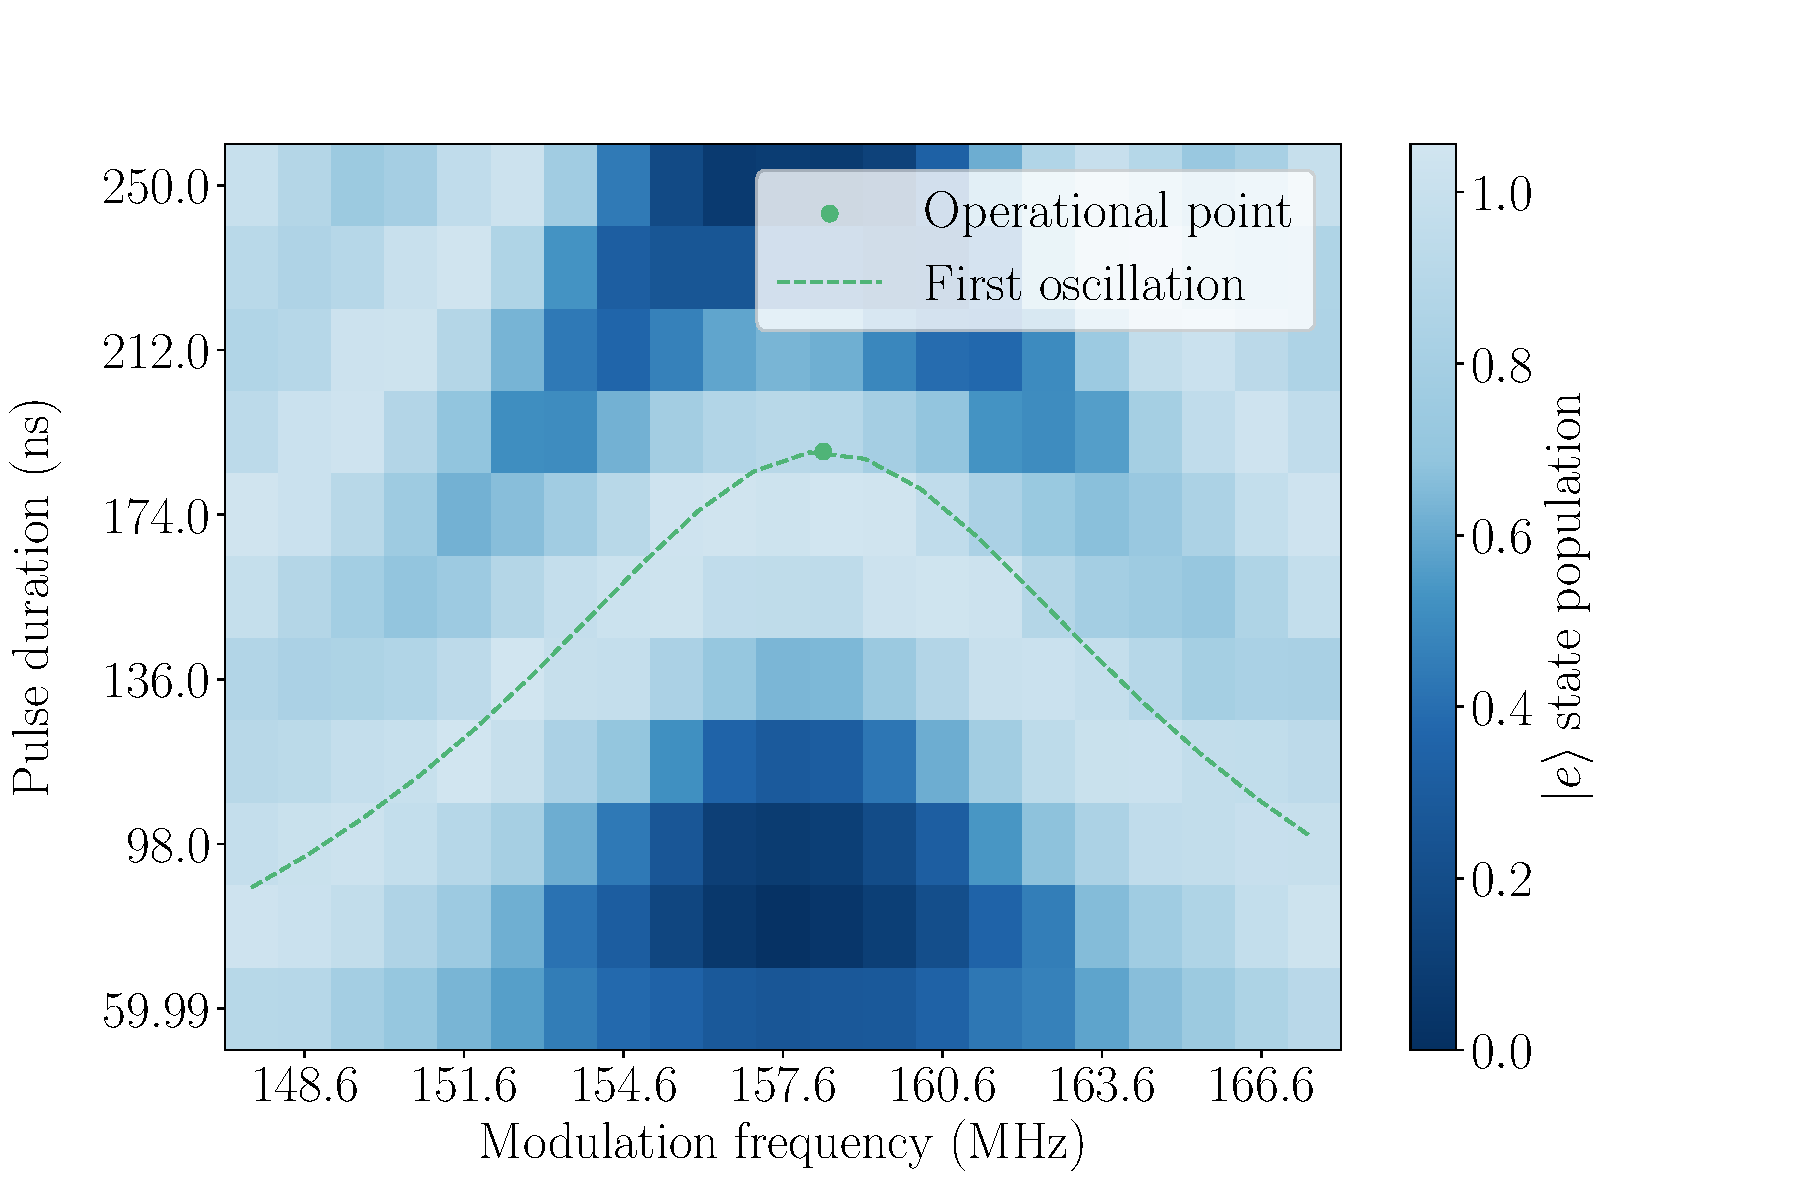
\includegraphics[width=0.8\linewidth]{Images//Chap3/Chevron_data.pdf}
    \caption{Data of the $eefg$ sideband transition between the two storage qubits}
    \label{fig:Chev_data}
\end{figure}

On \cref{fig:Chev_data} is also depicted the first oscillation period as a function of the detuning $\delta$, given by
\begin{equation}
    t = \frac{1}{\sqrt{4 g_0^2 + \delta^2}} . 
\end{equation}
\chapter{Graph States}
\label{Chap:graph_states}
\thispagestyle{fancy}

In quantum computing, a \emph{graph state} \cite{graph_state, rohde-graph-states} is a specific kind of multi-qubit state that can be depicted using a graph.
It can be understood as a summary of the interactions between particles, represented by the nodes.
At the same time, the adjacency matrix encodes the stabilizers of the state, which is a complete set of eigenvalue equations satisfied by the state. 

They are incredibly useful as they enable \emph{Measurement-Based Quantum Computing} (MBQC) \cite{MBQC}.
In MBQC, algorithms can be converted from gate sequences into a series of measurements and their respective bases. This allows for the execution of quantum algorithms through sequential measurement operations, providing an alternative implementation approach.

Graph states serve as foundational structures preceding \emph{cluster states} in quantum computing \cite{cluster_state}.
Cluster states, which are closely related to graph states, are essential for enabling universal quantum computation, as they provide the basis for \emph{Universal MBQC}.

\section{Definitions}
\label{Sec:graph_definition}

Graph states can be defined in two ways: through \emph{the stabilizer formalism} or using \emph{quantum circuits}.

\subsection{Stabilizer Formalism Definition}

A stabilizer is an operator under which the stabilised state is invariant, and the state is uniquely specified as the simultaneous $+1$ eigenstate of all $N$ stabilisers,
\begin{equation}
    S_i \ket{\psi} = \ket{\psi} \quad \forall i \in \{1, \ldots, N\} .
\end{equation}

A graph state, described by the graph $G = (V, E)$ has stabilizers of the form
\begin{equation}
    S_i = X_i \otimes_{j \in \mathcal{N}(i)} Z_j ,
\end{equation}
for each node $i$ of the graph, where $\mathcal{N}(i)$ denotes the neighbourhood of the node $i$.

\begin{figure}
    \centering
    

\tikzset{every picture/.style={line width=0.75pt}} %set default line width to 0.75pt        

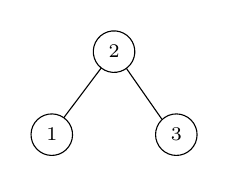
\begin{tikzpicture}[x=0.75pt,y=0.75pt,yscale=-1,xscale=1]
%uncomment if require: \path (0,300); %set diagram left start at 0, and has height of 300

%Shape: Circle [id:dp2524407142420394] 
\draw   (87.86,66.18) .. controls (84.45,70.52) and (78.17,71.28) .. (73.82,67.86) .. controls (69.48,64.45) and (68.72,58.17) .. (72.14,53.82) .. controls (75.55,49.48) and (81.83,48.72) .. (86.18,52.14) .. controls (90.52,55.55) and (91.28,61.83) .. (87.86,66.18) -- cycle ;
%Shape: Circle [id:dp4347791615686073] 
\draw   (41.84,94.21) .. controls (45.04,89.71) and (51.28,88.65) .. (55.79,91.84) .. controls (60.29,95.04) and (61.35,101.28) .. (58.16,105.79) .. controls (54.96,110.29) and (48.72,111.35) .. (44.21,108.16) .. controls (39.71,104.96) and (38.65,98.72) .. (41.84,94.21) -- cycle ;
%Shape: Circle [id:dp6645570183850392] 
\draw   (101.66,105.51) .. controls (98.61,100.91) and (99.88,94.7) .. (104.49,91.66) .. controls (109.09,88.61) and (115.3,89.88) .. (118.34,94.49) .. controls (121.39,99.09) and (120.12,105.3) .. (115.51,108.34) .. controls (110.91,111.39) and (104.7,110.12) .. (101.66,105.51) -- cycle ;
%Straight Lines [id:da7381513422337581] 
\draw    (85.94,68.05) -- (103,92.5) ;
%Straight Lines [id:da16373455646283308] 
\draw    (73.82,67.86) -- (55.79,91.84) ;

% Text Node
\draw (50,100) node  [font=\scriptsize]  {$1$};
% Text Node
\draw (80,60) node  [font=\scriptsize]  {$2$};
% Text Node
\draw (110,100) node  [font=\scriptsize]  {$3$};


\end{tikzpicture}
    \vspace{-1cm}
    \caption{A $3$-qubits linear graph state}
    \label{fig:simple_3_graph}
\end{figure}

As an example, consider the graph in \cref{fig:simple_3_graph}.
The graph state $\ket{G}$ has the stabilizers of the form
\begin{align}
    S_1 &= X_1 \otimes Z_2 , \notag \\
    S_2 &= Z_1 \otimes X_2 \otimes Z_3 , \label{eq:stabilizers} \\
    S_3 &= Z_2 \otimes X_3 , \notag
\end{align}
meaning that
\begin{equation}
    S_1 \ket{G} = 
    S_2 \ket{G} = 
    S_3 \ket{G} = 
    \ket{G} .
\end{equation}

\subsection{Quantum Circuit Definition}

An alternative and equivalent definition is the following.

Given a graph $G = (V, E)$, the graph state $\ket{G}$ is defined by
\begin{equation}
    \ket{G} = \prod_{\substack{\{ a, b \} \in E}} 
    CZ_{a, b} \ket{+}^{\otimes V} ,
\end{equation}
where $CZ_{a, b}$ is the controlled-phase operator between the vertices $a$ and $b$, and 
\begin{equation}
    \ket{+} = H \ket{0} = \frac{1}{\sqrt{2}} (\ket{0} + \ket{1}) .
\end{equation}

For instance, the state in \cref{fig:simple_3_graph} is
\begin{align}
    \ket{G} &=
    \prod_{\substack{\{ a, b \} \in E}} CZ_{a,b} \, H_1 H_2 H_3 \ket{000} =
    CZ_{1, 2} CZ_{2, 3} \ket{+++} \\
    &= \frac{1}{\sqrt{8}} 
    (\ket{000} + \ket{001} + \ket{010} - \ket{011} 
    + \ket{100} + \ket{101} - \ket{110} + \ket{111}) . \notag
\end{align}

It is easy to check that this state is indeed stabilized by the stabilizers $S_1$, $S_2$ and $S_3$ in \cref{eq:stabilizers}.
The equivalence of these definitions is demonstrated in the work \cite{graph_state}.

\section{Logical Operations on Graph States}
\label{Sec:log_operation_graph}

In \cref{chap:2_qubit_gates}, we delved into the protocols employed to implement two-qubit gates on our device.
Additionally, we explored the constraints that limit our ability to execute certain other gate operations.

This section provides a deeper exploration of gates applied to graph states. 
Frequently, rather than directly applying the specific gate, we utilize an alternative operation that produces an equivalent effect for a particular initial state.

For instance, the Hadamard gate $H$ and a $\pi / 2$ rotation around the $y$ axis are different gates, as we can see from the different unitary matrices
\begin{equation}
    H = \frac{1}{\sqrt{2}}
    \begin{bmatrix}
        1 & 1 \\
        1 & -1
    \end{bmatrix} , \quad
    R_y(\pi / 2) = \frac{1}{\sqrt{2}}
    \begin{bmatrix}
        1 & -1 \\
        1 & 1
    \end{bmatrix} .
\end{equation}

However, when these gates are applied to the initial state $\ket{0}$, they yield identical resulting states:
\begin{equation}
    H \ket{0} = R_y(\pi/2) \ket{0} = \ket{+} .
\end{equation}

In our experiments, given our inability to implement Hadamard gates directly on our device, we simulate its effect by executing rotations around the $y$ axis.
In general, the only single-qubit gates we can perform are rotations around the $x$, $y$, and $z$ axis. 
Fortunately, these gates often suffice for our purposes.

However, we need to be cautious as substituting all Hadamard gates with $\pi / 2$ rotations around the $y$ axis might not cover all situations. 
Take, for instance, the following:
\begin{equation}
    H H \ket{0} \neq
    R_y(\pi / 2) R_y(\pi / 2) \ket{0} .
\end{equation}

To ensure this equality holds, we need to alternate rotations of $\pi /2$ and $-\pi / 2$, as follows:
\begin{equation}
    H H \ket{0} =
    R_y(- \pi / 2) R_y(\pi / 2) \ket{0} .
\end{equation}

Now, let us revisit the two-qubit gates covered in \cref{chap:2_qubit_gates}:SWAP, CNOT, and SWAP.
We will analyze their implementation methods to achieve the intended graph state as the final outcome.

\subsection{CZ}

The simplest among these gates is the CZ gate, given that graph states are formulated based on this specific gate. 
If our goal is to obtain the state depicted in \cref{fig:CZ_graph} as an outcome, we aim to execute operations on the qubits such as:
\begin{equation}
    \begin{quantikz}
      \lstick{$\ket{0}_1$} & \gate{H} & \ctrl{1} & \qw \\
      \lstick{$\ket{0}_2$} & \gate{H} & \control{} & \qw
    \end{quantikz}
\end{equation}
Fortunately, replacing the Hadamard gates with $\pi/2$ rotations around the $y$ axis for both qubits accomplishes this task:
\begin{equation}
    \begin{quantikz}
      \lstick{$\ket{0}_1$} & \gate{Y_+} & \ctrl{1} & \qw \\
      \lstick{$\ket{0}_2$} & \gate{Y_+} & \control{} & \qw
    \end{quantikz}
\end{equation}

\begin{figure}
    \centering
    

\tikzset{every picture/.style={line width=0.75pt}} %set default line width to 0.75pt        

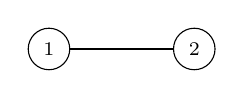
\begin{tikzpicture}[x=0.75pt,y=0.75pt,yscale=-1,xscale=1]
%uncomment if require: \path (0,162); %set diagram left start at 0, and has height of 162

%Shape: Circle [id:dp33085044400227215] 
\draw   (50,60) .. controls (50,54.48) and (54.48,50) .. (60,50) .. controls (65.52,50) and (70,54.48) .. (70,60) .. controls (70,65.52) and (65.52,70) .. (60,70) .. controls (54.48,70) and (50,65.52) .. (50,60) -- cycle ;
%Shape: Circle [id:dp45632065494671825] 
\draw   (120,60) .. controls (120,54.48) and (124.48,50) .. (130,50) .. controls (135.52,50) and (140,54.48) .. (140,60) .. controls (140,65.52) and (135.52,70) .. (130,70) .. controls (124.48,70) and (120,65.52) .. (120,60) -- cycle ;
%Straight Lines [id:da6274751888831748] 
\draw    (70,60) -- (120,60) ;

% Text Node
\draw (60,60) node  [font=\scriptsize]  {$1$};
% Text Node
\draw (130,60) node  [font=\scriptsize]  {$2$};


\end{tikzpicture}
    \vspace{-1cm}
    \caption{2-qubits linear graph}
    \label{fig:CZ_graph}
\end{figure}

From now on, we will use the following notation:
\begin{equation*}
    \begin{quantikz}
        \qw & \gate{Y_+} & \qw
    \end{quantikz}
    : R_y(+\pi/2) \, , \quad
    \begin{quantikz}
        \qw & \gate{Y_-} & \qw
    \end{quantikz}
    : R_y(-\pi/2)
\end{equation*}

\subsection{SWAP}

When studying the SWAP gate, it's crucial to consider its impact on the entanglement between the qubits involved and their connections to other qubits.
If our aim is to replicate the functionality of the following circuit
\begin{equation}
\label{eq:SWAP_circuit}
    \begin{quantikz}
      \lstick{$\ket{0}_1$} & \gate{H} & \ctrl{1}   & \qw      & \qw \\
      \lstick{$\ket{0}_2$} & \gate{H} & \control{} & \swap{1} & \qw \\
      \lstick{$\ket{0}_3$} & \gate{H} & \qw        & \targX{} & \qw
    \end{quantikz}
\end{equation}
we need to examine the changes occurring in the entanglement between qubits 1 and 2.
A visual representation is provided in \cref{fig:SWAP_graph}.
The SWAP gate effectively transfers the entanglement between the qubits, similarly to a simple swap in the numbering of the two qubits.

\begin{figure}[b]
    \centering
    

\tikzset{every picture/.style={line width=0.75pt}} %set default line width to 0.75pt        

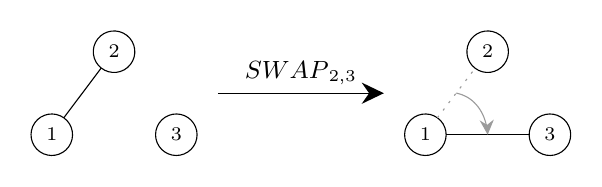
\begin{tikzpicture}[x=0.75pt,y=0.75pt,yscale=-1,xscale=1]
%uncomment if require: \path (0,162); %set diagram left start at 0, and has height of 162

%Shape: Circle [id:dp34495488497110016] 
\draw   (87.86,66.18) .. controls (84.45,70.52) and (78.17,71.28) .. (73.82,67.86) .. controls (69.48,64.45) and (68.72,58.17) .. (72.14,53.82) .. controls (75.55,49.48) and (81.83,48.72) .. (86.18,52.14) .. controls (90.52,55.55) and (91.28,61.83) .. (87.86,66.18) -- cycle ;
%Shape: Circle [id:dp2623874134924238] 
\draw   (41.84,94.21) .. controls (45.04,89.71) and (51.28,88.65) .. (55.79,91.84) .. controls (60.29,95.04) and (61.35,101.28) .. (58.16,105.79) .. controls (54.96,110.29) and (48.72,111.35) .. (44.21,108.16) .. controls (39.71,104.96) and (38.65,98.72) .. (41.84,94.21) -- cycle ;
%Shape: Circle [id:dp1378234889252382] 
\draw   (101.66,105.51) .. controls (98.61,100.91) and (99.88,94.7) .. (104.49,91.66) .. controls (109.09,88.61) and (115.3,89.88) .. (118.34,94.49) .. controls (121.39,99.09) and (120.12,105.3) .. (115.51,108.34) .. controls (110.91,111.39) and (104.7,110.12) .. (101.66,105.51) -- cycle ;
%Straight Lines [id:da18089547069059342] 
\draw    (73.82,67.86) -- (55.79,91.84) ;
%Shape: Circle [id:dp18245241155845826] 
\draw   (267.97,66.03) .. controls (264.64,70.44) and (258.37,71.31) .. (253.96,67.97) .. controls (249.56,64.64) and (248.69,58.37) .. (252.02,53.96) .. controls (255.36,49.56) and (261.63,48.69) .. (266.03,52.02) .. controls (270.44,55.36) and (271.31,61.63) .. (267.97,66.03) -- cycle ;
%Shape: Circle [id:dp8811036011863903] 
\draw   (221.84,94.21) .. controls (225.04,89.71) and (231.28,88.65) .. (235.78,91.84) .. controls (240.29,95.04) and (241.35,101.28) .. (238.15,105.78) .. controls (234.96,110.29) and (228.72,111.35) .. (224.21,108.15) .. controls (219.71,104.96) and (218.65,98.72) .. (221.84,94.21) -- cycle ;
%Straight Lines [id:da20903671041287875] 
\draw    (240,100) -- (280,100) ;
%Shape: Circle [id:dp9231143684580897] 
\draw   (281.82,105.75) .. controls (278.64,101.24) and (279.73,95) .. (284.24,91.82) .. controls (288.76,88.64) and (295,89.73) .. (298.18,94.24) .. controls (301.36,98.76) and (300.27,105) .. (295.75,108.18) .. controls (291.24,111.36) and (285,110.27) .. (281.82,105.75) -- cycle ;
%Straight Lines [id:da14252568592014891] 
\draw    (130,80) -- (207,80) ;
\draw [shift={(210,80)}, rotate = 180] [fill={rgb, 255:red, 0; green, 0; blue, 0 }  ][line width=0.08]  [draw opacity=0] (10.72,-5.15) -- (0,0) -- (10.72,5.15) -- (7.12,0) -- cycle    ;
%Straight Lines [id:da02595413260158763] 
\draw [color={rgb, 255:red, 155; green, 155; blue, 155 }  ,draw opacity=1 ] [dash pattern={on 0.84pt off 2.51pt}]  (235.78,91.84) -- (253.96,67.97) ;
%Curve Lines [id:da2796836261210731] 
\draw [color={rgb, 255:red, 155; green, 155; blue, 155 }  ,draw opacity=1 ]   (244.87,79.91) .. controls (252.27,81.36) and (258.18,87.56) .. (259.69,97.08) ;
\draw [shift={(260,100)}, rotate = 266.58] [fill={rgb, 255:red, 155; green, 155; blue, 155 }  ,fill opacity=1 ][line width=0.08]  [draw opacity=0] (7.14,-3.43) -- (0,0) -- (7.14,3.43) -- (4.74,0) -- cycle    ;

% Text Node
\draw (50,100) node  [font=\scriptsize]  {$1$};
% Text Node
\draw (80,60) node  [font=\scriptsize]  {$2$};
% Text Node
\draw (110,100) node  [font=\scriptsize]  {$3$};
% Text Node
\draw (230,100) node  [font=\scriptsize]  {$1$};
% Text Node
\draw (260,60) node  [font=\scriptsize]  {$2$};
% Text Node
\draw (290,100) node  [font=\scriptsize]  {$3$};
% Text Node
\draw (170,77) node [anchor=south] [inner sep=0.75pt]  [font=\small] [align=left] {$\displaystyle \text{SWAP}_{2,3}$};


\end{tikzpicture}
    \vspace{-1cm}
    \caption{Action of SWAP gate on entangling bonds with neighbouring qubits}
    \label{fig:SWAP_graph}
\end{figure}

Another aspect to consider is that we primarily implement the SWAP gate between a storage and an emitter. 
Consequently, in our example, we will designate qubit 3 as the emitter qubit. 
This means we're unable to perform single-qubit gates on it due to its rapid state decay.
We can execute the SPAW gate of \cref{fig:SWAP_graph} and generate an analogue final state by running the following protocol
\begin{equation}
    \begin{quantikz}
      \lstick{$\ket{0}_1$} & \gate{Y_+} & \ctrl{1}   & \qw      & \qw                & \qw \\
      \lstick{$\ket{0}_2$} & \gate{Y_+} & \control{} & \swap{1} & \gate{Y_+} & \qw \\
      \lstick{$\ket{0}_3$} & \qw                & \qw        & \targX{} & \qw                & \qw
    \end{quantikz}
\end{equation}
In the circuit architecture, the SWAP gate basically transfers both the state and the entangling bonds from qubit 2 to qubit 3.
Consequently, to achieve the state represented in \cref{eq:SWAP_circuit}, we need to further apply a Hadamard gate (or a $y$ rotation) on qubit 2 to bring it to the state $\ket{+}$.
Thus, the CNOT gate, followed by an Hadamard, effectively transfers all entanglement from the control qubit to the target qubit, while also entangling the two qubits, as depicted in \cref{fig:CNOT_graph}.

\begin{figure}
    \centering
    

\tikzset{every picture/.style={line width=0.75pt}} %set default line width to 0.75pt        

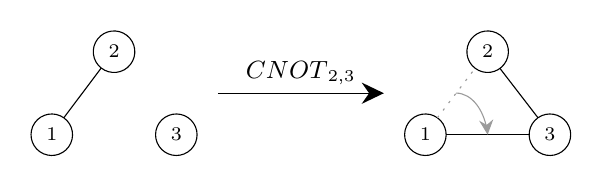
\begin{tikzpicture}[x=0.75pt,y=0.75pt,yscale=-1,xscale=1]
%uncomment if require: \path (0,162); %set diagram left start at 0, and has height of 162

%Shape: Circle [id:dp23417453743827976] 
\draw   (87.86,66.18) .. controls (84.45,70.52) and (78.17,71.28) .. (73.82,67.86) .. controls (69.48,64.45) and (68.72,58.17) .. (72.14,53.82) .. controls (75.55,49.48) and (81.83,48.72) .. (86.18,52.14) .. controls (90.52,55.55) and (91.28,61.83) .. (87.86,66.18) -- cycle ;
%Shape: Circle [id:dp011544140967992389] 
\draw   (41.84,94.21) .. controls (45.04,89.71) and (51.28,88.65) .. (55.79,91.84) .. controls (60.29,95.04) and (61.35,101.28) .. (58.16,105.79) .. controls (54.96,110.29) and (48.72,111.35) .. (44.21,108.16) .. controls (39.71,104.96) and (38.65,98.72) .. (41.84,94.21) -- cycle ;
%Shape: Circle [id:dp416194828283707] 
\draw   (101.66,105.51) .. controls (98.61,100.91) and (99.88,94.7) .. (104.49,91.66) .. controls (109.09,88.61) and (115.3,89.88) .. (118.34,94.49) .. controls (121.39,99.09) and (120.12,105.3) .. (115.51,108.34) .. controls (110.91,111.39) and (104.7,110.12) .. (101.66,105.51) -- cycle ;
%Straight Lines [id:da17802990060125945] 
\draw    (73.82,67.86) -- (55.79,91.84) ;
%Shape: Circle [id:dp026916354896634798] 
\draw   (267.97,66.03) .. controls (264.64,70.44) and (258.37,71.31) .. (253.96,67.97) .. controls (249.56,64.64) and (248.69,58.37) .. (252.02,53.96) .. controls (255.36,49.56) and (261.63,48.69) .. (266.03,52.02) .. controls (270.44,55.36) and (271.31,61.63) .. (267.97,66.03) -- cycle ;
%Shape: Circle [id:dp9684318791918579] 
\draw   (221.84,94.21) .. controls (225.04,89.71) and (231.28,88.65) .. (235.78,91.84) .. controls (240.29,95.04) and (241.35,101.28) .. (238.15,105.78) .. controls (234.96,110.29) and (228.72,111.35) .. (224.21,108.15) .. controls (219.71,104.96) and (218.65,98.72) .. (221.84,94.21) -- cycle ;
%Straight Lines [id:da43300710363321016] 
\draw    (265.93,68.05) -- (284.24,91.82) ;
%Shape: Circle [id:dp3103272610346469] 
\draw   (281.82,105.75) .. controls (278.64,101.24) and (279.73,95) .. (284.24,91.82) .. controls (288.76,88.64) and (295,89.73) .. (298.18,94.24) .. controls (301.36,98.76) and (300.27,105) .. (295.75,108.18) .. controls (291.24,111.36) and (285,110.27) .. (281.82,105.75) -- cycle ;
%Straight Lines [id:da6511414638961373] 
\draw    (130,80) -- (207,80) ;
\draw [shift={(210,80)}, rotate = 180] [fill={rgb, 255:red, 0; green, 0; blue, 0 }  ][line width=0.08]  [draw opacity=0] (10.72,-5.15) -- (0,0) -- (10.72,5.15) -- (7.12,0) -- cycle    ;
%Straight Lines [id:da1905731404703308] 
\draw    (240,100) -- (280,100) ;
%Straight Lines [id:da19331622592606712] 
\draw [color={rgb, 255:red, 155; green, 155; blue, 155 }  ,draw opacity=1 ] [dash pattern={on 0.84pt off 2.51pt}]  (235.78,91.84) -- (253.96,67.97) ;
%Curve Lines [id:da4343842529052825] 
\draw [color={rgb, 255:red, 155; green, 155; blue, 155 }  ,draw opacity=1 ]   (244.87,79.91) .. controls (252.59,80.17) and (257.91,88.06) .. (259.59,97.12) ;
\draw [shift={(260,100)}, rotate = 264.4] [fill={rgb, 255:red, 155; green, 155; blue, 155 }  ,fill opacity=1 ][line width=0.08]  [draw opacity=0] (7.14,-3.43) -- (0,0) -- (7.14,3.43) -- (4.74,0) -- cycle    ;

% Text Node
\draw (50,100) node  [font=\scriptsize]  {$1$};
% Text Node
\draw (80,60) node  [font=\scriptsize]  {$2$};
% Text Node
\draw (110,100) node  [font=\scriptsize]  {$3$};
% Text Node
\draw (230,100) node  [font=\scriptsize]  {$1$};
% Text Node
\draw (260,60) node  [font=\scriptsize]  {$2$};
% Text Node
\draw (290,100) node  [font=\scriptsize]  {$3$};
% Text Node
\draw (170,77) node [anchor=south] [inner sep=0.75pt]  [font=\small] [align=left] {$\displaystyle \text{CNOT}_{2,3}$};


\end{tikzpicture}
    \vspace{-1cm}
    \caption{Action of CNOT gate on the entangling bonds of the target qubit}
    \label{fig:CNOT_graph}
\end{figure}

\subsection{CNOT}

The situation changes once more when dealing with the CNOT gate.
The following equivalence between the resulting quantum states can be easily checked:
\begin{equation}
    \begin{quantikz}
      \lstick{$\ket{0}_1$} & \gate{H} & \ctrl{1}   & \qw      & \qw \\
      \lstick{$\ket{0}_2$} & \gate{H} & \control{} & \ctrl{1} & \qw \\
      \lstick{$\ket{0}_3$} & \gate{H} & \qw        & \targ{}  & \qw
    \end{quantikz}
    \; = \;
    \begin{quantikz}
      \lstick{$\ket{0}_1$} & \gate{H} & \ctrl{2}   & \qw         & \qw \\
      \lstick{$\ket{0}_2$} & \gate{H} & \qw        & \ctrl{1}    & \qw \\
      \lstick{$\ket{0}_3$} & \gate{H} & \control{} & \control{}  & \qw
    \end{quantikz}
\end{equation}
It's worth noting that the equivalence is solely between outcomes, assuming the initial state is $\ket{000}$, not between the quantum circuits themselves.
In practice, the unitary matrices representing the actions of the two circuits would differ.

To replicate the action of this gate and achieve the same resulting graph state, precise attention must be paid to the phase signs in rotations around the $y$ axis.
We will maintain the assumption that qubit 3 serves as an emitter qubit, as previously established in the case of the SWAP gate.
The executable sequence of gates on our device is the following:
\begin{equation}
    \begin{quantikz}
      \lstick{$\ket{0}_1$} & \gate{Y_+}  & \ctrl{1}   & \qw         & \qw                 & \qw \\
      \lstick{$\ket{0}_2$} & \gate{Y_-} & \control{} & \ctrl{1}    & \gate{Y_+} & \qw \\
      \lstick{$\ket{0}_3$} & \qw                 & \qw        & \targ{}     & \qw                 & \qw
    \end{quantikz}
\end{equation}

Typically, when multiple Hadamard gates are applied to the same qubit without resetting it through a SWAP gate with an emitter, it becomes necessary to alternate the rotation's sign around the $y$ axis.
Intuitively, this adjustment is needed because applying two rotations is not equivalent to applying two Hadamard gates, even when the initial state is $\ket{0}$.
To accurately represent this scenario, we might need to implement a sequence resembling the following:
\begin{equation}
    H H \ket{0} =
    R_y(- \pi / 2) R_y(\pi / 2) \ket{0} =
    R_y(\pi / 2) R_y(-\pi / 2) \ket{0} .
\end{equation}

Moreover, it's important to note that the effect of a $y$ rotation and the Hadamard gate differs when applied to the state $\ket{1}$:
\begin{equation}
    H \ket{1} = \ket{-} , \quad
    R_y(\pi / 2) \ket{1} = - \ket{-} .
\end{equation}

Hence, intuitively, it becomes crucial to alternate the signs of the $\pi/2$ rotation around the $y$ axis, ensuring that the final rotation within the sequence is positive. 
This alternating pattern ensures proper alignment with the intended quantum operations, particularly when dealing with sequences involving multiple rotations or Hadamard gates on the same qubit.
\section{Tree Graph State}
\label{chap:tree_graph_state}
\thispagestyle{fancy}

The work by Y. Zhan \emph{et al.} \cite{tree_graph_state} highlighted the central challenge of reliably transmitting quantum signals through noisy and lossy channels.

While conventional quantum repeater proposals relied on heraled entanglement generation and two-way classical signaling, recent proposals have been made towards leveraging \emph{photonic graph states} to overcome these challenges.
These graph-state-based quantum repeaters \cite{One_way_quantum_repeaters} present a promising alternative by employing quantum encoding to address photon losses and operational errors, ultimately bypassing the necessity for extensive quantum memory coherence times.

However, generating such photonic graph states traditionally demands substantial resources and intricate methodologies involving linear optics and a considerable amounts of auxiliary qubits.
Despite this challenge, various schemes have been proposed for deterministic generation of these states, including \emph{tree graph} and \emph{repeater graph states}.

This section will look into how we can create these graph states using our device. 
In the previous sections, we have described the key steps to make specific types of graphs and entanglement bonds between the qubits in our device.
Now, we will explore how to use these tools to generate these graph states, with potential future applications in quantum networking.

\subsection{(2, 2) Tree Graph State}
\label{sec:2_2_tree}

\begin{figure}
    \centering
    

\tikzset{every picture/.style={line width=0.75pt}} %set default line width to 0.75pt        

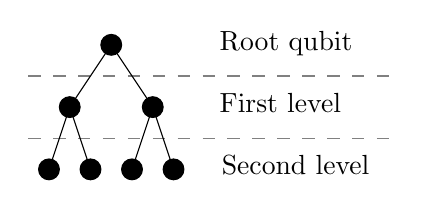
\begin{tikzpicture}[x=0.75pt,y=0.75pt,yscale=-1,xscale=1]
%uncomment if require: \path (0,300); %set diagram left start at 0, and has height of 300

%Straight Lines [id:da8426905590991587] 
\draw [color={rgb, 255:red, 128; green, 128; blue, 128 }  ,draw opacity=1 ] [dash pattern={on 4.5pt off 4.5pt}]  (60,85) -- (240,85) ;
%Straight Lines [id:da5406148798931413] 
\draw [color={rgb, 255:red, 128; green, 128; blue, 128 }  ,draw opacity=1 ] [dash pattern={on 4.5pt off 4.5pt}]  (60,55) -- (240,55) ;
%Straight Lines [id:da0310472865739988] 
\draw    (80,70) -- (90,100) ;
%Straight Lines [id:da44724908569705224] 
\draw    (80,70) -- (100,40) ;
%Shape: Circle [id:dp9646050192410193] 
\draw  [fill={rgb, 255:red, 0; green, 0; blue, 0 }  ,fill opacity=1 ] (95,40) .. controls (95,37.24) and (97.24,35) .. (100,35) .. controls (102.76,35) and (105,37.24) .. (105,40) .. controls (105,42.76) and (102.76,45) .. (100,45) .. controls (97.24,45) and (95,42.76) .. (95,40) -- cycle ;
%Shape: Circle [id:dp9987430184128605] 
\draw  [fill={rgb, 255:red, 0; green, 0; blue, 0 }  ,fill opacity=1 ] (105,100) .. controls (105,97.24) and (107.24,95) .. (110,95) .. controls (112.76,95) and (115,97.24) .. (115,100) .. controls (115,102.76) and (112.76,105) .. (110,105) .. controls (107.24,105) and (105,102.76) .. (105,100) -- cycle ;
%Shape: Circle [id:dp5327923177036115] 
\draw  [fill={rgb, 255:red, 0; green, 0; blue, 0 }  ,fill opacity=1 ] (125,100) .. controls (125,97.24) and (127.24,95) .. (130,95) .. controls (132.76,95) and (135,97.24) .. (135,100) .. controls (135,102.76) and (132.76,105) .. (130,105) .. controls (127.24,105) and (125,102.76) .. (125,100) -- cycle ;
%Shape: Circle [id:dp07874792740386194] 
\draw  [fill={rgb, 255:red, 0; green, 0; blue, 0 }  ,fill opacity=1 ] (115,70) .. controls (115,67.24) and (117.24,65) .. (120,65) .. controls (122.76,65) and (125,67.24) .. (125,70) .. controls (125,72.76) and (122.76,75) .. (120,75) .. controls (117.24,75) and (115,72.76) .. (115,70) -- cycle ;
%Shape: Circle [id:dp827553292195197] 
\draw  [fill={rgb, 255:red, 0; green, 0; blue, 0 }  ,fill opacity=1 ] (65,100) .. controls (65,97.24) and (67.24,95) .. (70,95) .. controls (72.76,95) and (75,97.24) .. (75,100) .. controls (75,102.76) and (72.76,105) .. (70,105) .. controls (67.24,105) and (65,102.76) .. (65,100) -- cycle ;
%Shape: Circle [id:dp9737971224660668] 
\draw  [fill={rgb, 255:red, 0; green, 0; blue, 0 }  ,fill opacity=1 ] (85,100) .. controls (85,97.24) and (87.24,95) .. (90,95) .. controls (92.76,95) and (95,97.24) .. (95,100) .. controls (95,102.76) and (92.76,105) .. (90,105) .. controls (87.24,105) and (85,102.76) .. (85,100) -- cycle ;
%Shape: Circle [id:dp3888180938045467] 
\draw  [fill={rgb, 255:red, 0; green, 0; blue, 0 }  ,fill opacity=1 ] (75,70) .. controls (75,67.24) and (77.24,65) .. (80,65) .. controls (82.76,65) and (85,67.24) .. (85,70) .. controls (85,72.76) and (82.76,75) .. (80,75) .. controls (77.24,75) and (75,72.76) .. (75,70) -- cycle ;
%Straight Lines [id:da09087177582110562] 
\draw    (80,70) -- (70,100) ;
%Straight Lines [id:da9701309593546271] 
\draw    (100,40) -- (120,70) ;
%Straight Lines [id:da7485547301936679] 
\draw    (110,100) -- (120,70) ;
%Straight Lines [id:da005037302745795835] 
\draw    (120,70) -- (130,100) ;

% Text Node
\draw (151,32) node [anchor=north west][inner sep=0.75pt]   [align=left] {Root qubit};
% Text Node
\draw (151,62) node [anchor=north west][inner sep=0.75pt]   [align=left] {First level};
% Text Node
\draw (152,92) node [anchor=north west][inner sep=0.75pt]   [align=left] {Second level};


\end{tikzpicture}
    \vspace{-1cm}
    \caption{Representation of $(2, 2)$ tree graph state}
    \label{fig:2_2_graph}
\end{figure}

The term \emph{$(n, m)$ tree graph state} refers to a tree structure where the initial qubit, known as the root qubit, links to $n$ other qubits, each of which is connected to $m$ additional qubits.
Specifically, we'll focus on examining a $(2, 2)$ tree graph state, visually represented in \cref{fig:2_2_graph}.

The tree graph state holds importance in one-way quantum repeater protocols as one can encode a logical state on the entire graph by running operations between a data qubit and the root node.
This resilience, requiring only a subset of essential photons for loss correction \cite{Why_tree_graph_state}, enables qubit transmission even if some photons are lost, ensuring reliable communication despite potential losses.
Hence, it is crucial to create the tree graph state while ensuring the root remains stored within one of our qubits, as it is necessary for Bell state measurements, enabling the encoding of the intended state for transmission.

We will begin by outlining the protocol employed to create the initial branch of the $(2, 2)$ tree graph state.
Initially, we generate the root qubit for the tree state using a straightforward $\pi/2$ $y$ rotation.
In the circuit diagram, the first quantum wire represents the root of the tree, stored within one of the physical qubits of our device.
The second quantum wire represents the second physical qubit, while the remaining wires symbolize flying photons.
\begin{equation}
\label{eq:1_branch_implementation}
    \begin{quantikz}
      \lstick{$\ket{0}_{S1}$} & \gate{Y_+}\slice[style=black]{\textbf{(a)}}  & \qw      & \qw  & \qw & \ctrl{1}  & \qw & \qw   & \qw      & \qw & \qw &  \qw & \qw & \qw \\
      \lstick{$\ket{0}_{S2}$} & \gate{Y_+} & \ctrl{1} & \gate{Y_-} \slice[style=black]{\textbf{(b)}} &  \qw   & \control{}  & \qw \slice[style=black]{\textbf{(c)}} & \qw   & \ctrl{2} & \gate{Y_+}\slice[style=black]{\textbf{(d)}} & \qw & \swap{3} & \qw \slice[style=black]{\textbf{(e)}} & \qw \\
      \lstick{$\ket{0}_{P1}$} & \qw                 & \targ{}      & \qw           & \qw       & \qw     & \qw   & \qw   & \qw  & \qw                 & \qw & \qw & \qw & \qw\\
      \lstick{$\ket{0}_{P2}$} & \qw                 & \qw          & \qw           & \qw       & \qw     & \qw   & \qw   & \targ{}      & \qw                 & \qw & \qw & \qw & \qw  \\
      \lstick{$\ket{0}_{P3}$} & \qw                 & \qw      & \qw          & \qw        & \qw      & \qw  & \qw   & \qw      & \qw                 & \qw & \targX{} & \qw & \qw
    \end{quantikz}
\end{equation}

\begin{figure}[b]
    \centering
    

\tikzset{every picture/.style={line width=0.75pt}} %set default line width to 0.75pt        

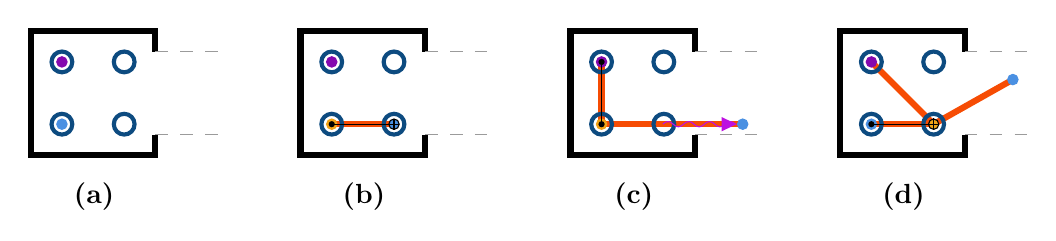
\begin{tikzpicture}[x=0.75pt,y=0.75pt,yscale=-1,xscale=1]
%uncomment if require: \path (0,134); %set diagram left start at 0, and has height of 134

%Shape: Circle [id:dp8634696649139634] 
\draw  [color={rgb, 255:red, 13; green, 75; blue, 128 }  ,draw opacity=1 ][line width=1.5]  (30,35) .. controls (30,32.24) and (32.24,30) .. (35,30) .. controls (37.76,30) and (40,32.24) .. (40,35) .. controls (40,37.76) and (37.76,40) .. (35,40) .. controls (32.24,40) and (30,37.76) .. (30,35) -- cycle ;
%Shape: Circle [id:dp3171229884283615] 
\draw  [color={rgb, 255:red, 13; green, 75; blue, 128 }  ,draw opacity=1 ][line width=1.5]  (30,65) .. controls (30,62.24) and (32.24,60) .. (35,60) .. controls (37.76,60) and (40,62.24) .. (40,65) .. controls (40,67.76) and (37.76,70) .. (35,70) .. controls (32.24,70) and (30,67.76) .. (30,65) -- cycle ;
%Shape: Circle [id:dp8674284799713297] 
\draw  [color={rgb, 255:red, 13; green, 75; blue, 128 }  ,draw opacity=1 ][line width=1.5]  (60,65) .. controls (60,62.24) and (62.24,60) .. (65,60) .. controls (67.76,60) and (70,62.24) .. (70,65) .. controls (70,67.76) and (67.76,70) .. (65,70) .. controls (62.24,70) and (60,67.76) .. (60,65) -- cycle ;
%Shape: Circle [id:dp13408530876145808] 
\draw  [color={rgb, 255:red, 13; green, 75; blue, 128 }  ,draw opacity=1 ][line width=1.5]  (60,35) .. controls (60,32.24) and (62.24,30) .. (65,30) .. controls (67.76,30) and (70,32.24) .. (70,35) .. controls (70,37.76) and (67.76,40) .. (65,40) .. controls (62.24,40) and (60,37.76) .. (60,35) -- cycle ;
%Shape: Square [id:dp47099491834906715] 
\draw  [line width=2.25]  (20,20) -- (80,20) -- (80,80) -- (20,80) -- cycle ;
%Straight Lines [id:da0834144987419978] 
\draw [color={rgb, 255:red, 255; green, 255; blue, 255 }  ,draw opacity=1 ][line width=3]    (80,30) -- (80,70) ;

%Shape: Circle [id:dp5113434790777113] 
\draw  [color={rgb, 255:red, 132; green, 9; blue, 175 }  ,draw opacity=1 ][fill={rgb, 255:red, 132; green, 9; blue, 175 }  ,fill opacity=1 ] (32.5,35) .. controls (32.5,33.62) and (33.62,32.5) .. (35,32.5) .. controls (36.38,32.5) and (37.5,33.62) .. (37.5,35) .. controls (37.5,36.38) and (36.38,37.5) .. (35,37.5) .. controls (33.62,37.5) and (32.5,36.38) .. (32.5,35) -- cycle ;
%Straight Lines [id:da46112915361915263] 
\draw [color={rgb, 255:red, 155; green, 155; blue, 155 }  ,draw opacity=1 ] [dash pattern={on 4.5pt off 4.5pt}]  (80,30) -- (110,30) ;
%Straight Lines [id:da9498457389457537] 
\draw [color={rgb, 255:red, 155; green, 155; blue, 155 }  ,draw opacity=1 ] [dash pattern={on 4.5pt off 4.5pt}]  (80,70) -- (110,70) ;
%Shape: Circle [id:dp9873280063938384] 
\draw  [color={rgb, 255:red, 74; green, 144; blue, 226 }  ,draw opacity=1 ][fill={rgb, 255:red, 74; green, 144; blue, 226 }  ,fill opacity=1 ] (32.5,65) .. controls (32.5,63.62) and (33.62,62.5) .. (35,62.5) .. controls (36.38,62.5) and (37.5,63.62) .. (37.5,65) .. controls (37.5,66.38) and (36.38,67.5) .. (35,67.5) .. controls (33.62,67.5) and (32.5,66.38) .. (32.5,65) -- cycle ;
%Shape: Circle [id:dp6431718269187471] 
\draw  [color={rgb, 255:red, 132; green, 9; blue, 175 }  ,draw opacity=1 ][fill={rgb, 255:red, 132; green, 9; blue, 175 }  ,fill opacity=1 ] (162.5,35) .. controls (162.5,33.62) and (163.62,32.5) .. (165,32.5) .. controls (166.38,32.5) and (167.5,33.62) .. (167.5,35) .. controls (167.5,36.38) and (166.38,37.5) .. (165,37.5) .. controls (163.62,37.5) and (162.5,36.38) .. (162.5,35) -- cycle ;
%Shape: Circle [id:dp21383549781911027] 
\draw  [color={rgb, 255:red, 13; green, 75; blue, 128 }  ,draw opacity=1 ][line width=1.5]  (160,35) .. controls (160,32.24) and (162.24,30) .. (165,30) .. controls (167.76,30) and (170,32.24) .. (170,35) .. controls (170,37.76) and (167.76,40) .. (165,40) .. controls (162.24,40) and (160,37.76) .. (160,35) -- cycle ;
%Shape: Circle [id:dp3789153251551227] 
\draw  [color={rgb, 255:red, 13; green, 75; blue, 128 }  ,draw opacity=1 ][line width=1.5]  (190,35) .. controls (190,32.24) and (192.24,30) .. (195,30) .. controls (197.76,30) and (200,32.24) .. (200,35) .. controls (200,37.76) and (197.76,40) .. (195,40) .. controls (192.24,40) and (190,37.76) .. (190,35) -- cycle ;
%Shape: Square [id:dp28884126483287875] 
\draw  [line width=2.25]  (150,20) -- (210,20) -- (210,80) -- (150,80) -- cycle ;
%Straight Lines [id:da7068966502224133] 
\draw [color={rgb, 255:red, 255; green, 255; blue, 255 }  ,draw opacity=1 ][line width=3]    (210,30) -- (210,70) ;

%Straight Lines [id:da5803960409811918] 
\draw [color={rgb, 255:red, 155; green, 155; blue, 155 }  ,draw opacity=1 ] [dash pattern={on 4.5pt off 4.5pt}]  (210,30) -- (240,30) ;
%Straight Lines [id:da7547530202356005] 
\draw [color={rgb, 255:red, 155; green, 155; blue, 155 }  ,draw opacity=1 ] [dash pattern={on 4.5pt off 4.5pt}]  (210,70) -- (240,70) ;
%Straight Lines [id:da6849475869613678] 
\draw [color={rgb, 255:red, 246; green, 76; blue, 4 }  ,draw opacity=1 ][line width=2.25]    (165,65) -- (195,65) ;
%Shape: Circle [id:dp7155137713689077] 
\draw  [color={rgb, 255:red, 241; green, 163; blue, 23 }  ,draw opacity=1 ][fill={rgb, 255:red, 241; green, 163; blue, 23 }  ,fill opacity=1 ] (162.5,65) .. controls (162.5,63.62) and (163.62,62.5) .. (165,62.5) .. controls (166.38,62.5) and (167.5,63.62) .. (167.5,65) .. controls (167.5,66.38) and (166.38,67.5) .. (165,67.5) .. controls (163.62,67.5) and (162.5,66.38) .. (162.5,65) -- cycle ;
%Shape: Circle [id:dp2190211775758546] 
\draw  [color={rgb, 255:red, 0; green, 0; blue, 0 }  ,draw opacity=1 ][fill={rgb, 255:red, 74; green, 144; blue, 226 }  ,fill opacity=1 ] (192.5,65) .. controls (192.5,63.62) and (193.62,62.5) .. (195,62.5) .. controls (196.38,62.5) and (197.5,63.62) .. (197.5,65) .. controls (197.5,66.38) and (196.38,67.5) .. (195,67.5) .. controls (193.62,67.5) and (192.5,66.38) .. (192.5,65) -- cycle ;
%Straight Lines [id:da5019530038163004] 
\draw    (195,62.5) -- (195,68) ;
%Straight Lines [id:da023533720970719596] 
\draw    (197.5,65) -- (192.5,65) ;
%Shape: Circle [id:dp463883226646705] 
\draw  [draw opacity=0][fill={rgb, 255:red, 0; green, 0; blue, 0 }  ,fill opacity=1 ] (163.5,65) .. controls (163.5,64.17) and (164.17,63.5) .. (165,63.5) .. controls (165.83,63.5) and (166.5,64.17) .. (166.5,65) .. controls (166.5,65.83) and (165.83,66.5) .. (165,66.5) .. controls (164.17,66.5) and (163.5,65.83) .. (163.5,65) -- cycle ;
%Shape: Circle [id:dp2941797335933385] 
\draw  [color={rgb, 255:red, 13; green, 75; blue, 128 }  ,draw opacity=1 ][line width=1.5]  (190,65) .. controls (190,62.24) and (192.24,60) .. (195,60) .. controls (197.76,60) and (200,62.24) .. (200,65) .. controls (200,67.76) and (197.76,70) .. (195,70) .. controls (192.24,70) and (190,67.76) .. (190,65) -- cycle ;
%Shape: Circle [id:dp19508965820109148] 
\draw  [color={rgb, 255:red, 13; green, 75; blue, 128 }  ,draw opacity=1 ][line width=1.5]  (160,65) .. controls (160,62.24) and (162.24,60) .. (165,60) .. controls (167.76,60) and (170,62.24) .. (170,65) .. controls (170,67.76) and (167.76,70) .. (165,70) .. controls (162.24,70) and (160,67.76) .. (160,65) -- cycle ;
%Straight Lines [id:da36230041238257815] 
\draw    (165,65) -- (195,65) ;
%Shape: Square [id:dp22566803032018268] 
\draw  [line width=2.25]  (280,20) -- (340,20) -- (340,80) -- (280,80) -- cycle ;
%Straight Lines [id:da8610306823319624] 
\draw [color={rgb, 255:red, 255; green, 255; blue, 255 }  ,draw opacity=1 ][line width=3]    (340,30) -- (340,70) ;

%Straight Lines [id:da9138577476417785] 
\draw [color={rgb, 255:red, 246; green, 76; blue, 4 }  ,draw opacity=1 ][line width=2.25]    (295,65) -- (363,65) ;
%Straight Lines [id:da9264747080487808] 
\draw [color={rgb, 255:red, 246; green, 76; blue, 4 }  ,draw opacity=1 ][line width=2.25]    (295,35) -- (295,65) ;
%Shape: Circle [id:dp826290588201388] 
\draw  [color={rgb, 255:red, 132; green, 9; blue, 175 }  ,draw opacity=1 ][fill={rgb, 255:red, 132; green, 9; blue, 175 }  ,fill opacity=1 ] (292.5,35) .. controls (292.5,33.62) and (293.62,32.5) .. (295,32.5) .. controls (296.38,32.5) and (297.5,33.62) .. (297.5,35) .. controls (297.5,36.38) and (296.38,37.5) .. (295,37.5) .. controls (293.62,37.5) and (292.5,36.38) .. (292.5,35) -- cycle ;
%Shape: Circle [id:dp9454665293887276] 
\draw  [color={rgb, 255:red, 13; green, 75; blue, 128 }  ,draw opacity=1 ][line width=1.5]  (290,35) .. controls (290,32.24) and (292.24,30) .. (295,30) .. controls (297.76,30) and (300,32.24) .. (300,35) .. controls (300,37.76) and (297.76,40) .. (295,40) .. controls (292.24,40) and (290,37.76) .. (290,35) -- cycle ;
%Shape: Circle [id:dp9678738407214998] 
\draw  [color={rgb, 255:red, 13; green, 75; blue, 128 }  ,draw opacity=1 ][line width=1.5]  (290,65) .. controls (290,62.24) and (292.24,60) .. (295,60) .. controls (297.76,60) and (300,62.24) .. (300,65) .. controls (300,67.76) and (297.76,70) .. (295,70) .. controls (292.24,70) and (290,67.76) .. (290,65) -- cycle ;
%Shape: Circle [id:dp11638652073637779] 
\draw  [color={rgb, 255:red, 13; green, 75; blue, 128 }  ,draw opacity=1 ][line width=1.5]  (320,65) .. controls (320,62.24) and (322.24,60) .. (325,60) .. controls (327.76,60) and (330,62.24) .. (330,65) .. controls (330,67.76) and (327.76,70) .. (325,70) .. controls (322.24,70) and (320,67.76) .. (320,65) -- cycle ;
%Shape: Circle [id:dp8846315373556948] 
\draw  [color={rgb, 255:red, 13; green, 75; blue, 128 }  ,draw opacity=1 ][line width=1.5]  (320,35) .. controls (320,32.24) and (322.24,30) .. (325,30) .. controls (327.76,30) and (330,32.24) .. (330,35) .. controls (330,37.76) and (327.76,40) .. (325,40) .. controls (322.24,40) and (320,37.76) .. (320,35) -- cycle ;
%Straight Lines [id:da15824455233757484] 
\draw [color={rgb, 255:red, 155; green, 155; blue, 155 }  ,draw opacity=1 ] [dash pattern={on 4.5pt off 4.5pt}]  (340,30) -- (370,30) ;
%Straight Lines [id:da08275578074384338] 
\draw [color={rgb, 255:red, 155; green, 155; blue, 155 }  ,draw opacity=1 ] [dash pattern={on 4.5pt off 4.5pt}]  (340,70) -- (370,70) ;
%Shape: Circle [id:dp4480793960053918] 
\draw  [color={rgb, 255:red, 241; green, 163; blue, 23 }  ,draw opacity=1 ][fill={rgb, 255:red, 241; green, 163; blue, 23 }  ,fill opacity=1 ] (292.5,65) .. controls (292.5,63.62) and (293.62,62.5) .. (295,62.5) .. controls (296.38,62.5) and (297.5,63.62) .. (297.5,65) .. controls (297.5,66.38) and (296.38,67.5) .. (295,67.5) .. controls (293.62,67.5) and (292.5,66.38) .. (292.5,65) -- cycle ;
%Shape: Circle [id:dp4701197125733043] 
\draw  [color={rgb, 255:red, 74; green, 144; blue, 226 }  ,draw opacity=1 ][fill={rgb, 255:red, 74; green, 144; blue, 226 }  ,fill opacity=1 ] (360.5,65) .. controls (360.5,63.62) and (361.62,62.5) .. (363,62.5) .. controls (364.38,62.5) and (365.5,63.62) .. (365.5,65) .. controls (365.5,66.38) and (364.38,67.5) .. (363,67.5) .. controls (361.62,67.5) and (360.5,66.38) .. (360.5,65) -- cycle ;
%Shape: Circle [id:dp36402367761201493] 
\draw  [draw opacity=0][fill={rgb, 255:red, 0; green, 0; blue, 0 }  ,fill opacity=1 ] (293.5,65) .. controls (293.5,64.17) and (294.17,63.5) .. (295,63.5) .. controls (295.83,63.5) and (296.5,64.17) .. (296.5,65) .. controls (296.5,65.83) and (295.83,66.5) .. (295,66.5) .. controls (294.17,66.5) and (293.5,65.83) .. (293.5,65) -- cycle ;
%Shape: Circle [id:dp7874046855771671] 
\draw  [draw opacity=0][fill={rgb, 255:red, 0; green, 0; blue, 0 }  ,fill opacity=1 ] (293.5,35) .. controls (293.5,34.17) and (294.17,33.5) .. (295,33.5) .. controls (295.83,33.5) and (296.5,34.17) .. (296.5,35) .. controls (296.5,35.83) and (295.83,36.5) .. (295,36.5) .. controls (294.17,36.5) and (293.5,35.83) .. (293.5,35) -- cycle ;
%Straight Lines [id:da2898778351352036] 
\draw    (295,35) -- (295,65) ;
%Straight Lines [id:da7752313531562761] 
\draw [color={rgb, 255:red, 189; green, 16; blue, 224 }  ,draw opacity=1 ]   (324.5,65) .. controls (326.17,63.33) and (327.83,63.33) .. (329.5,65) .. controls (331.17,66.67) and (332.83,66.67) .. (334.5,65) .. controls (336.17,63.33) and (337.83,63.33) .. (339.5,65) .. controls (341.17,66.67) and (342.83,66.67) .. (344.5,65) .. controls (346.17,63.33) and (347.83,63.33) .. (349.5,65) .. controls (351.17,66.67) and (352.83,66.67) .. (354.5,65) .. controls (356.17,63.33) and (357.83,63.33) .. (359.5,65) -- (360,65) -- (360,65) ;
%Straight Lines [id:da9446040288212432] 
\draw [color={rgb, 255:red, 189; green, 16; blue, 224 }  ,draw opacity=1 ]   (354.25,65) -- (357,65) ;
\draw [shift={(360,65)}, rotate = 180] [fill={rgb, 255:red, 189; green, 16; blue, 224 }  ,fill opacity=1 ][line width=0.08]  [draw opacity=0] (7.14,-3.43) -- (0,0) -- (7.14,3.43) -- cycle    ;
%Straight Lines [id:da4458315367718473] 
\draw [color={rgb, 255:red, 246; green, 76; blue, 4 }  ,draw opacity=1 ][line width=2.25]    (425,65) -- (455,65) ;
%Straight Lines [id:da6417507071495968] 
\draw [color={rgb, 255:red, 246; green, 76; blue, 4 }  ,draw opacity=1 ][line width=2.25]    (425,35) -- (455,65) ;
%Shape: Square [id:dp19892382898236483] 
\draw  [line width=2.25]  (410,20) -- (470,20) -- (470,80) -- (410,80) -- cycle ;
%Straight Lines [id:da8211154882339877] 
\draw [color={rgb, 255:red, 255; green, 255; blue, 255 }  ,draw opacity=1 ][line width=3]    (470,30) -- (470,70) ;

%Straight Lines [id:da1226594004392908] 
\draw [color={rgb, 255:red, 246; green, 76; blue, 4 }  ,draw opacity=1 ][line width=2.25]    (493.17,43.5) -- (455,65) ;
%Shape: Circle [id:dp25607475791662804] 
\draw  [color={rgb, 255:red, 132; green, 9; blue, 175 }  ,draw opacity=1 ][fill={rgb, 255:red, 132; green, 9; blue, 175 }  ,fill opacity=1 ] (422.5,35) .. controls (422.5,33.62) and (423.62,32.5) .. (425,32.5) .. controls (426.38,32.5) and (427.5,33.62) .. (427.5,35) .. controls (427.5,36.38) and (426.38,37.5) .. (425,37.5) .. controls (423.62,37.5) and (422.5,36.38) .. (422.5,35) -- cycle ;
%Shape: Circle [id:dp7472085667416201] 
\draw  [color={rgb, 255:red, 13; green, 75; blue, 128 }  ,draw opacity=1 ][line width=1.5]  (420,35) .. controls (420,32.24) and (422.24,30) .. (425,30) .. controls (427.76,30) and (430,32.24) .. (430,35) .. controls (430,37.76) and (427.76,40) .. (425,40) .. controls (422.24,40) and (420,37.76) .. (420,35) -- cycle ;
%Shape: Circle [id:dp6105247050154898] 
\draw  [color={rgb, 255:red, 13; green, 75; blue, 128 }  ,draw opacity=1 ][line width=1.5]  (420,65) .. controls (420,62.24) and (422.24,60) .. (425,60) .. controls (427.76,60) and (430,62.24) .. (430,65) .. controls (430,67.76) and (427.76,70) .. (425,70) .. controls (422.24,70) and (420,67.76) .. (420,65) -- cycle ;
%Shape: Circle [id:dp10304227171071978] 
\draw  [color={rgb, 255:red, 13; green, 75; blue, 128 }  ,draw opacity=1 ][line width=1.5]  (450,65) .. controls (450,62.24) and (452.24,60) .. (455,60) .. controls (457.76,60) and (460,62.24) .. (460,65) .. controls (460,67.76) and (457.76,70) .. (455,70) .. controls (452.24,70) and (450,67.76) .. (450,65) -- cycle ;
%Shape: Circle [id:dp4134298947687973] 
\draw  [color={rgb, 255:red, 13; green, 75; blue, 128 }  ,draw opacity=1 ][line width=1.5]  (450,35) .. controls (450,32.24) and (452.24,30) .. (455,30) .. controls (457.76,30) and (460,32.24) .. (460,35) .. controls (460,37.76) and (457.76,40) .. (455,40) .. controls (452.24,40) and (450,37.76) .. (450,35) -- cycle ;
%Straight Lines [id:da05857273260240248] 
\draw [color={rgb, 255:red, 155; green, 155; blue, 155 }  ,draw opacity=1 ] [dash pattern={on 4.5pt off 4.5pt}]  (470,30) -- (500,30) ;
%Straight Lines [id:da8515467099208363] 
\draw [color={rgb, 255:red, 155; green, 155; blue, 155 }  ,draw opacity=1 ] [dash pattern={on 4.5pt off 4.5pt}]  (470,70) -- (500,70) ;
%Shape: Circle [id:dp3385953242829104] 
\draw  [color={rgb, 255:red, 74; green, 144; blue, 226 }  ,draw opacity=1 ][fill={rgb, 255:red, 74; green, 144; blue, 226 }  ,fill opacity=1 ] (422.5,65) .. controls (422.5,63.62) and (423.62,62.5) .. (425,62.5) .. controls (426.38,62.5) and (427.5,63.62) .. (427.5,65) .. controls (427.5,66.38) and (426.38,67.5) .. (425,67.5) .. controls (423.62,67.5) and (422.5,66.38) .. (422.5,65) -- cycle ;
%Shape: Circle [id:dp6520838784850642] 
\draw  [color={rgb, 255:red, 0; green, 0; blue, 0 }  ,draw opacity=1 ][fill={rgb, 255:red, 241; green, 163; blue, 23 }  ,fill opacity=1 ] (452.5,65) .. controls (452.5,63.62) and (453.62,62.5) .. (455,62.5) .. controls (456.38,62.5) and (457.5,63.62) .. (457.5,65) .. controls (457.5,66.38) and (456.38,67.5) .. (455,67.5) .. controls (453.62,67.5) and (452.5,66.38) .. (452.5,65) -- cycle ;
%Straight Lines [id:da9256744917784654] 
\draw    (455,62) -- (455,67.5) ;
%Straight Lines [id:da28871784610038775] 
\draw    (425,65) -- (455,65) ;
%Straight Lines [id:da9178977220598342] 
\draw    (457.5,65) -- (452.5,65) ;
%Shape: Circle [id:dp7957363186924172] 
\draw  [draw opacity=0][fill={rgb, 255:red, 0; green, 0; blue, 0 }  ,fill opacity=1 ] (423.5,65) .. controls (423.5,64.17) and (424.17,63.5) .. (425,63.5) .. controls (425.83,63.5) and (426.5,64.17) .. (426.5,65) .. controls (426.5,65.83) and (425.83,66.5) .. (425,66.5) .. controls (424.17,66.5) and (423.5,65.83) .. (423.5,65) -- cycle ;
%Shape: Circle [id:dp6977350768470425] 
\draw  [color={rgb, 255:red, 74; green, 144; blue, 226 }  ,draw opacity=1 ][fill={rgb, 255:red, 74; green, 144; blue, 226 }  ,fill opacity=1 ] (490.67,43.5) .. controls (490.67,42.12) and (491.79,41) .. (493.17,41) .. controls (494.55,41) and (495.67,42.12) .. (495.67,43.5) .. controls (495.67,44.88) and (494.55,46) .. (493.17,46) .. controls (491.79,46) and (490.67,44.88) .. (490.67,43.5) -- cycle ;

% Text Node
\draw (50.5,92) node [anchor=north] [inner sep=0.75pt]   [align=left] {\textbf{(a)}};
% Text Node
\draw (180.5,92) node [anchor=north] [inner sep=0.75pt]   [align=left] {\textbf{(b)}};
% Text Node
\draw (310.5,92) node [anchor=north] [inner sep=0.75pt]   [align=left] {\textbf{(c)}};
% Text Node
\draw (440.5,92) node [anchor=north] [inner sep=0.75pt]   [align=left] {\textbf{(d)}};


\end{tikzpicture}
    \vspace{-1cm}
    \caption{Visual implementation of first branch of the $(2, 2)$ tree graph state}
    \label{fig:1_branch_tree}
\end{figure}

Fig.~\ref{fig:1_branch_tree} illustrates the visual progression occurring within the device.

Should we emit all nodes except for the root, we can replicate the process to generate the second and final branch of the intended quantum state.
The circuit illustrating the entire implementation of the tree graph state is presented below. 
Notably, the initial two quantum wires maintain their role as the first and second storage qubits.
Meanwhile, the remaining six wires signify the six additional vertices in the state, functioning as flying qubits in our configuration.
\begin{equation}
\label{eq:tree_implementation}
    \begin{quantikz}[column sep=0.4cm]
      \lstick{$\ket{0}_{S1}$} & \gate{Y_+} & \qw & \qw & \ctrl{1} & \qw & \qw & \qw & \qw & \qw & \qw & \ctrl{1} & \qw & \qw & \qw & \qw \\
      \lstick{$\ket{0}_{S2}$} & \gate{Y_+} & \ctrl{1} & \gate{Y_-} & \control{} & \ctrl{2} & \gate{Y_+} & \swap{3} & \gate{Y_+} & \ctrl{4} & \gate{Y_-} & \control{} & \ctrl{5} & \gate{Y_+} & \swap{6} & \qw \\
      \lstick{$\ket{0}_{P1}$} & \qw & \targ{} & \qw & \qw & \qw & \qw & \qw & \qw & \qw & \qw & \qw & \qw & \qw & \qw & \qw \\
      \lstick{$\ket{0}_{P2}$} & \qw & \qw & \qw & \qw & \targ{} & \qw & \qw & \qw & \qw & \qw & \qw & \qw & \qw & \qw & \qw \\
      \lstick{$\ket{0}_{P3}$} & \qw & \qw & \qw & \qw & \qw & \qw & \targX{} & \qw & \qw & \qw & \qw & \qw & \qw & \qw & \qw \\
      \lstick{$\ket{0}_{P4}$} & \qw & \qw & \qw & \qw & \qw & \qw & \qw & \qw & \targ{} & \qw & \qw & \qw & \qw & \qw & \qw \\
      \lstick{$\ket{0}_{P5}$} & \qw & \qw & \qw & \qw & \qw & \qw & \qw & \qw & \qw & \qw & \qw & \targ{} & \qw & \qw & \qw \\
      \lstick{$\ket{0}_{P6}$} & \qw & \qw & \qw & \qw & \qw & \qw & \qw & \qw & \qw & \qw & \qw & \qw & \qw & \targX{} & \qw
    \end{quantikz}
\end{equation}

The state generated with the previous circuit is equivalent to the following graph state.

\begin{equation}
\label{eq:tree_graph_state}
    \begin{quantikz}
        \lstick{$\ket{0}_{S1}$} & \gate{H}  & \ctrl{2}  & \qw  & \qw  & \ctrl{5}  & \qw  & \qw  & \qw \\
        \lstick{$\ket{0}_{P1}$} & \gate{H}  & \qw  & \qw  & \ctrl{1}  & \qw  & \qw  & \qw  & \qw \\
        \lstick{$\ket{0}_{P2}$} & \gate{H}  & \control{}  & \ctrl{1}  & \control{}  & \qw  & \qw  & \qw  & \qw \\
        \lstick{$\ket{0}_{P3}$} & \gate{H}  & \qw  & \control{}  & \qw  & \qw  & \qw  & \qw  & \qw \\
        \lstick{$\ket{0}_{P4}$} & \gate{H}  & \qw  & \qw  & \qw  & \qw  & \qw  & \ctrl{1}  & \qw \\
        \lstick{$\ket{0}_{P5}$} & \gate{H}  & \qw  & \qw  & \qw  & \control{}  & \ctrl{1}  & \control{}  & \qw \\
        \lstick{$\ket{0}_{P6}$} & \gate{H}  & \qw  & \qw  & \qw  & \qw  & \control{}  & \qw  & \qw
    \end{quantikz}
\end{equation}

Fig.~\ref{fig:final_tree_implementation} shows the final state we would get if we were to implement \cref{eq:tree_implementation} on our device, labelling the vertices according to the numbering in the equation.

% \begin{figure}
%     \centering
%     

\tikzset{every picture/.style={line width=0.75pt}} %set default line width to 0.75pt        

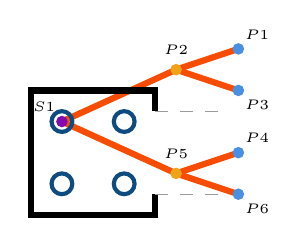
\begin{tikzpicture}[x=0.75pt,y=0.75pt,yscale=-1,xscale=1]
%uncomment if require: \path (0,182); %set diagram left start at 0, and has height of 182

%Straight Lines [id:da47465656152714486] 
\draw [color={rgb, 255:red, 246; green, 76; blue, 4 }  ,draw opacity=1 ][line width=2.25]    (315,75) -- (370,50) ;
%Shape: Square [id:dp7338884259497895] 
\draw  [line width=2.25]  (300,60) -- (360,60) -- (360,120) -- (300,120) -- cycle ;
%Straight Lines [id:da6927342142359094] 
\draw [color={rgb, 255:red, 255; green, 255; blue, 255 }  ,draw opacity=1 ][line width=3]    (360,70) -- (360,110) ;

%Straight Lines [id:da6098087629891208] 
\draw [color={rgb, 255:red, 246; green, 76; blue, 4 }  ,draw opacity=1 ][line width=2.25]    (370,50) -- (400,60) ;
%Straight Lines [id:da9586171017662504] 
\draw [color={rgb, 255:red, 246; green, 76; blue, 4 }  ,draw opacity=1 ][line width=2.25]    (400,40) -- (370,50) ;
%Straight Lines [id:da9166685119570428] 
\draw [color={rgb, 255:red, 246; green, 76; blue, 4 }  ,draw opacity=1 ][line width=2.25]    (370,100) -- (400,110) ;
%Straight Lines [id:da12081008351293132] 
\draw [color={rgb, 255:red, 246; green, 76; blue, 4 }  ,draw opacity=1 ][line width=2.25]    (315,75) -- (370,100) ;
%Straight Lines [id:da43191174777453967] 
\draw [color={rgb, 255:red, 246; green, 76; blue, 4 }  ,draw opacity=1 ][line width=2.25]    (400,90) -- (370,100) ;
%Shape: Circle [id:dp41145059566786146] 
\draw  [color={rgb, 255:red, 132; green, 9; blue, 175 }  ,draw opacity=1 ][fill={rgb, 255:red, 132; green, 9; blue, 175 }  ,fill opacity=1 ] (312.5,75) .. controls (312.5,73.62) and (313.62,72.5) .. (315,72.5) .. controls (316.38,72.5) and (317.5,73.62) .. (317.5,75) .. controls (317.5,76.38) and (316.38,77.5) .. (315,77.5) .. controls (313.62,77.5) and (312.5,76.38) .. (312.5,75) -- cycle ;
%Shape: Circle [id:dp5320458710332802] 
\draw  [color={rgb, 255:red, 13; green, 75; blue, 128 }  ,draw opacity=1 ][line width=1.5]  (310,75) .. controls (310,72.24) and (312.24,70) .. (315,70) .. controls (317.76,70) and (320,72.24) .. (320,75) .. controls (320,77.76) and (317.76,80) .. (315,80) .. controls (312.24,80) and (310,77.76) .. (310,75) -- cycle ;
%Shape: Circle [id:dp3617334287188755] 
\draw  [color={rgb, 255:red, 13; green, 75; blue, 128 }  ,draw opacity=1 ][line width=1.5]  (310,105) .. controls (310,102.24) and (312.24,100) .. (315,100) .. controls (317.76,100) and (320,102.24) .. (320,105) .. controls (320,107.76) and (317.76,110) .. (315,110) .. controls (312.24,110) and (310,107.76) .. (310,105) -- cycle ;
%Shape: Circle [id:dp07731016955749404] 
\draw  [color={rgb, 255:red, 13; green, 75; blue, 128 }  ,draw opacity=1 ][line width=1.5]  (340,105) .. controls (340,102.24) and (342.24,100) .. (345,100) .. controls (347.76,100) and (350,102.24) .. (350,105) .. controls (350,107.76) and (347.76,110) .. (345,110) .. controls (342.24,110) and (340,107.76) .. (340,105) -- cycle ;
%Shape: Circle [id:dp16339127645713447] 
\draw  [color={rgb, 255:red, 13; green, 75; blue, 128 }  ,draw opacity=1 ][line width=1.5]  (340,75) .. controls (340,72.24) and (342.24,70) .. (345,70) .. controls (347.76,70) and (350,72.24) .. (350,75) .. controls (350,77.76) and (347.76,80) .. (345,80) .. controls (342.24,80) and (340,77.76) .. (340,75) -- cycle ;
%Straight Lines [id:da6337075775283348] 
\draw [color={rgb, 255:red, 155; green, 155; blue, 155 }  ,draw opacity=1 ] [dash pattern={on 4.5pt off 4.5pt}]  (360,70) -- (390,70) ;
%Straight Lines [id:da4062260044648891] 
\draw [color={rgb, 255:red, 155; green, 155; blue, 155 }  ,draw opacity=1 ] [dash pattern={on 4.5pt off 4.5pt}]  (360,110) -- (390,110) ;
%Shape: Circle [id:dp34879830519151855] 
\draw  [color={rgb, 255:red, 74; green, 144; blue, 226 }  ,draw opacity=1 ][fill={rgb, 255:red, 74; green, 144; blue, 226 }  ,fill opacity=1 ] (397.5,110) .. controls (397.5,108.62) and (398.62,107.5) .. (400,107.5) .. controls (401.38,107.5) and (402.5,108.62) .. (402.5,110) .. controls (402.5,111.38) and (401.38,112.5) .. (400,112.5) .. controls (398.62,112.5) and (397.5,111.38) .. (397.5,110) -- cycle ;
%Shape: Circle [id:dp05200913272998542] 
\draw  [color={rgb, 255:red, 241; green, 163; blue, 23 }  ,draw opacity=1 ][fill={rgb, 255:red, 241; green, 163; blue, 23 }  ,fill opacity=1 ] (367.5,100) .. controls (367.5,98.62) and (368.62,97.5) .. (370,97.5) .. controls (371.38,97.5) and (372.5,98.62) .. (372.5,100) .. controls (372.5,101.38) and (371.38,102.5) .. (370,102.5) .. controls (368.62,102.5) and (367.5,101.38) .. (367.5,100) -- cycle ;
%Shape: Circle [id:dp43357034961897] 
\draw  [color={rgb, 255:red, 74; green, 144; blue, 226 }  ,draw opacity=1 ][fill={rgb, 255:red, 74; green, 144; blue, 226 }  ,fill opacity=1 ] (397.5,40) .. controls (397.5,38.62) and (398.62,37.5) .. (400,37.5) .. controls (401.38,37.5) and (402.5,38.62) .. (402.5,40) .. controls (402.5,41.38) and (401.38,42.5) .. (400,42.5) .. controls (398.62,42.5) and (397.5,41.38) .. (397.5,40) -- cycle ;
%Shape: Circle [id:dp7842924247669173] 
\draw  [color={rgb, 255:red, 241; green, 163; blue, 23 }  ,draw opacity=1 ][fill={rgb, 255:red, 241; green, 163; blue, 23 }  ,fill opacity=1 ] (367.5,50) .. controls (367.5,48.62) and (368.62,47.5) .. (370,47.5) .. controls (371.38,47.5) and (372.5,48.62) .. (372.5,50) .. controls (372.5,51.38) and (371.38,52.5) .. (370,52.5) .. controls (368.62,52.5) and (367.5,51.38) .. (367.5,50) -- cycle ;
%Shape: Circle [id:dp5315495156196338] 
\draw  [color={rgb, 255:red, 74; green, 144; blue, 226 }  ,draw opacity=1 ][fill={rgb, 255:red, 74; green, 144; blue, 226 }  ,fill opacity=1 ] (397.5,60) .. controls (397.5,58.62) and (398.62,57.5) .. (400,57.5) .. controls (401.38,57.5) and (402.5,58.62) .. (402.5,60) .. controls (402.5,61.38) and (401.38,62.5) .. (400,62.5) .. controls (398.62,62.5) and (397.5,61.38) .. (397.5,60) -- cycle ;
%Shape: Circle [id:dp9788740260400791] 
\draw  [color={rgb, 255:red, 74; green, 144; blue, 226 }  ,draw opacity=1 ][fill={rgb, 255:red, 74; green, 144; blue, 226 }  ,fill opacity=1 ] (397.5,90) .. controls (397.5,88.62) and (398.62,87.5) .. (400,87.5) .. controls (401.38,87.5) and (402.5,88.62) .. (402.5,90) .. controls (402.5,91.38) and (401.38,92.5) .. (400,92.5) .. controls (398.62,92.5) and (397.5,91.38) .. (397.5,90) -- cycle ;

% Text Node
\draw (313,71.6) node [anchor=south east] [inner sep=0.75pt]  [font=\tiny]  {$S1$};
% Text Node
\draw (370,44.1) node [anchor=south] [inner sep=0.75pt]  [font=\tiny]  {$P2$};
% Text Node
\draw (402,36.6) node [anchor=south west] [inner sep=0.75pt]  [font=\tiny]  {$P1$};
% Text Node
\draw (402,63.4) node [anchor=north west][inner sep=0.75pt]  [font=\tiny]  {$P3$};
% Text Node
\draw (402,86.6) node [anchor=south west] [inner sep=0.75pt]  [font=\tiny]  {$P4$};
% Text Node
\draw (370,94.1) node [anchor=south] [inner sep=0.75pt]  [font=\tiny]  {$P5$};
% Text Node
\draw (402,113.4) node [anchor=north west][inner sep=0.75pt]  [font=\tiny]  {$P6$};


\end{tikzpicture}
%     \vspace{-1cm}
%     \caption{Outcome state after implementing % \cref{eq:tree_implementation}}
%     \label{fig:final_tree_implementation}
% \end{figure}

\begin{figure}
    \begin{minipage}{0.45\textwidth}
        \centering
        

\tikzset{every picture/.style={line width=0.75pt}} %set default line width to 0.75pt        

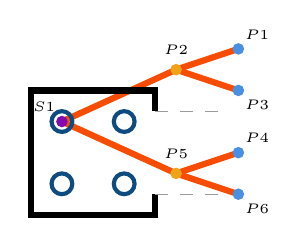
\begin{tikzpicture}[x=0.75pt,y=0.75pt,yscale=-1,xscale=1]
%uncomment if require: \path (0,182); %set diagram left start at 0, and has height of 182

%Straight Lines [id:da47465656152714486] 
\draw [color={rgb, 255:red, 246; green, 76; blue, 4 }  ,draw opacity=1 ][line width=2.25]    (315,75) -- (370,50) ;
%Shape: Square [id:dp7338884259497895] 
\draw  [line width=2.25]  (300,60) -- (360,60) -- (360,120) -- (300,120) -- cycle ;
%Straight Lines [id:da6927342142359094] 
\draw [color={rgb, 255:red, 255; green, 255; blue, 255 }  ,draw opacity=1 ][line width=3]    (360,70) -- (360,110) ;

%Straight Lines [id:da6098087629891208] 
\draw [color={rgb, 255:red, 246; green, 76; blue, 4 }  ,draw opacity=1 ][line width=2.25]    (370,50) -- (400,60) ;
%Straight Lines [id:da9586171017662504] 
\draw [color={rgb, 255:red, 246; green, 76; blue, 4 }  ,draw opacity=1 ][line width=2.25]    (400,40) -- (370,50) ;
%Straight Lines [id:da9166685119570428] 
\draw [color={rgb, 255:red, 246; green, 76; blue, 4 }  ,draw opacity=1 ][line width=2.25]    (370,100) -- (400,110) ;
%Straight Lines [id:da12081008351293132] 
\draw [color={rgb, 255:red, 246; green, 76; blue, 4 }  ,draw opacity=1 ][line width=2.25]    (315,75) -- (370,100) ;
%Straight Lines [id:da43191174777453967] 
\draw [color={rgb, 255:red, 246; green, 76; blue, 4 }  ,draw opacity=1 ][line width=2.25]    (400,90) -- (370,100) ;
%Shape: Circle [id:dp41145059566786146] 
\draw  [color={rgb, 255:red, 132; green, 9; blue, 175 }  ,draw opacity=1 ][fill={rgb, 255:red, 132; green, 9; blue, 175 }  ,fill opacity=1 ] (312.5,75) .. controls (312.5,73.62) and (313.62,72.5) .. (315,72.5) .. controls (316.38,72.5) and (317.5,73.62) .. (317.5,75) .. controls (317.5,76.38) and (316.38,77.5) .. (315,77.5) .. controls (313.62,77.5) and (312.5,76.38) .. (312.5,75) -- cycle ;
%Shape: Circle [id:dp5320458710332802] 
\draw  [color={rgb, 255:red, 13; green, 75; blue, 128 }  ,draw opacity=1 ][line width=1.5]  (310,75) .. controls (310,72.24) and (312.24,70) .. (315,70) .. controls (317.76,70) and (320,72.24) .. (320,75) .. controls (320,77.76) and (317.76,80) .. (315,80) .. controls (312.24,80) and (310,77.76) .. (310,75) -- cycle ;
%Shape: Circle [id:dp3617334287188755] 
\draw  [color={rgb, 255:red, 13; green, 75; blue, 128 }  ,draw opacity=1 ][line width=1.5]  (310,105) .. controls (310,102.24) and (312.24,100) .. (315,100) .. controls (317.76,100) and (320,102.24) .. (320,105) .. controls (320,107.76) and (317.76,110) .. (315,110) .. controls (312.24,110) and (310,107.76) .. (310,105) -- cycle ;
%Shape: Circle [id:dp07731016955749404] 
\draw  [color={rgb, 255:red, 13; green, 75; blue, 128 }  ,draw opacity=1 ][line width=1.5]  (340,105) .. controls (340,102.24) and (342.24,100) .. (345,100) .. controls (347.76,100) and (350,102.24) .. (350,105) .. controls (350,107.76) and (347.76,110) .. (345,110) .. controls (342.24,110) and (340,107.76) .. (340,105) -- cycle ;
%Shape: Circle [id:dp16339127645713447] 
\draw  [color={rgb, 255:red, 13; green, 75; blue, 128 }  ,draw opacity=1 ][line width=1.5]  (340,75) .. controls (340,72.24) and (342.24,70) .. (345,70) .. controls (347.76,70) and (350,72.24) .. (350,75) .. controls (350,77.76) and (347.76,80) .. (345,80) .. controls (342.24,80) and (340,77.76) .. (340,75) -- cycle ;
%Straight Lines [id:da6337075775283348] 
\draw [color={rgb, 255:red, 155; green, 155; blue, 155 }  ,draw opacity=1 ] [dash pattern={on 4.5pt off 4.5pt}]  (360,70) -- (390,70) ;
%Straight Lines [id:da4062260044648891] 
\draw [color={rgb, 255:red, 155; green, 155; blue, 155 }  ,draw opacity=1 ] [dash pattern={on 4.5pt off 4.5pt}]  (360,110) -- (390,110) ;
%Shape: Circle [id:dp34879830519151855] 
\draw  [color={rgb, 255:red, 74; green, 144; blue, 226 }  ,draw opacity=1 ][fill={rgb, 255:red, 74; green, 144; blue, 226 }  ,fill opacity=1 ] (397.5,110) .. controls (397.5,108.62) and (398.62,107.5) .. (400,107.5) .. controls (401.38,107.5) and (402.5,108.62) .. (402.5,110) .. controls (402.5,111.38) and (401.38,112.5) .. (400,112.5) .. controls (398.62,112.5) and (397.5,111.38) .. (397.5,110) -- cycle ;
%Shape: Circle [id:dp05200913272998542] 
\draw  [color={rgb, 255:red, 241; green, 163; blue, 23 }  ,draw opacity=1 ][fill={rgb, 255:red, 241; green, 163; blue, 23 }  ,fill opacity=1 ] (367.5,100) .. controls (367.5,98.62) and (368.62,97.5) .. (370,97.5) .. controls (371.38,97.5) and (372.5,98.62) .. (372.5,100) .. controls (372.5,101.38) and (371.38,102.5) .. (370,102.5) .. controls (368.62,102.5) and (367.5,101.38) .. (367.5,100) -- cycle ;
%Shape: Circle [id:dp43357034961897] 
\draw  [color={rgb, 255:red, 74; green, 144; blue, 226 }  ,draw opacity=1 ][fill={rgb, 255:red, 74; green, 144; blue, 226 }  ,fill opacity=1 ] (397.5,40) .. controls (397.5,38.62) and (398.62,37.5) .. (400,37.5) .. controls (401.38,37.5) and (402.5,38.62) .. (402.5,40) .. controls (402.5,41.38) and (401.38,42.5) .. (400,42.5) .. controls (398.62,42.5) and (397.5,41.38) .. (397.5,40) -- cycle ;
%Shape: Circle [id:dp7842924247669173] 
\draw  [color={rgb, 255:red, 241; green, 163; blue, 23 }  ,draw opacity=1 ][fill={rgb, 255:red, 241; green, 163; blue, 23 }  ,fill opacity=1 ] (367.5,50) .. controls (367.5,48.62) and (368.62,47.5) .. (370,47.5) .. controls (371.38,47.5) and (372.5,48.62) .. (372.5,50) .. controls (372.5,51.38) and (371.38,52.5) .. (370,52.5) .. controls (368.62,52.5) and (367.5,51.38) .. (367.5,50) -- cycle ;
%Shape: Circle [id:dp5315495156196338] 
\draw  [color={rgb, 255:red, 74; green, 144; blue, 226 }  ,draw opacity=1 ][fill={rgb, 255:red, 74; green, 144; blue, 226 }  ,fill opacity=1 ] (397.5,60) .. controls (397.5,58.62) and (398.62,57.5) .. (400,57.5) .. controls (401.38,57.5) and (402.5,58.62) .. (402.5,60) .. controls (402.5,61.38) and (401.38,62.5) .. (400,62.5) .. controls (398.62,62.5) and (397.5,61.38) .. (397.5,60) -- cycle ;
%Shape: Circle [id:dp9788740260400791] 
\draw  [color={rgb, 255:red, 74; green, 144; blue, 226 }  ,draw opacity=1 ][fill={rgb, 255:red, 74; green, 144; blue, 226 }  ,fill opacity=1 ] (397.5,90) .. controls (397.5,88.62) and (398.62,87.5) .. (400,87.5) .. controls (401.38,87.5) and (402.5,88.62) .. (402.5,90) .. controls (402.5,91.38) and (401.38,92.5) .. (400,92.5) .. controls (398.62,92.5) and (397.5,91.38) .. (397.5,90) -- cycle ;

% Text Node
\draw (313,71.6) node [anchor=south east] [inner sep=0.75pt]  [font=\tiny]  {$S1$};
% Text Node
\draw (370,44.1) node [anchor=south] [inner sep=0.75pt]  [font=\tiny]  {$P2$};
% Text Node
\draw (402,36.6) node [anchor=south west] [inner sep=0.75pt]  [font=\tiny]  {$P1$};
% Text Node
\draw (402,63.4) node [anchor=north west][inner sep=0.75pt]  [font=\tiny]  {$P3$};
% Text Node
\draw (402,86.6) node [anchor=south west] [inner sep=0.75pt]  [font=\tiny]  {$P4$};
% Text Node
\draw (370,94.1) node [anchor=south] [inner sep=0.75pt]  [font=\tiny]  {$P5$};
% Text Node
\draw (402,113.4) node [anchor=north west][inner sep=0.75pt]  [font=\tiny]  {$P6$};


\end{tikzpicture}
        \vspace{-1cm}
        \caption{Outcome state after implementing \cref{eq:tree_implementation}}
        \label{fig:final_tree_implementation}
    \end{minipage}
    \hspace{1cm}
    \begin{minipage}{0.45\textwidth}
        \centering
        

\tikzset{every picture/.style={line width=0.75pt}} %set default line width to 0.75pt        

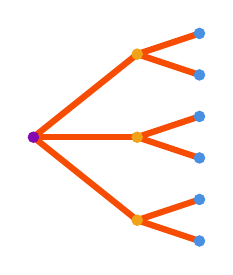
\begin{tikzpicture}[x=0.75pt,y=0.75pt,yscale=-1,xscale=1]
%uncomment if require: \path (0,182); %set diagram left start at 0, and has height of 182

%Straight Lines [id:da5808000645086375] 
\draw [color={rgb, 255:red, 246; green, 76; blue, 4 }  ,draw opacity=1 ][line width=2.25]    (360,70) -- (390,80) ;
%Straight Lines [id:da18975921226163972] 
\draw [color={rgb, 255:red, 246; green, 76; blue, 4 }  ,draw opacity=1 ][line width=2.25]    (390,60) -- (360,70) ;
%Straight Lines [id:da6595221878479601] 
\draw [color={rgb, 255:red, 246; green, 76; blue, 4 }  ,draw opacity=1 ][line width=2.25]    (360,110) -- (390,120) ;
%Straight Lines [id:da5683498370526975] 
\draw [color={rgb, 255:red, 246; green, 76; blue, 4 }  ,draw opacity=1 ][line width=2.25]    (390,100) -- (360,110) ;
%Straight Lines [id:da9165166451633462] 
\draw [color={rgb, 255:red, 246; green, 76; blue, 4 }  ,draw opacity=1 ][line width=2.25]    (360,30) -- (390,40) ;
%Straight Lines [id:da7926013585642647] 
\draw [color={rgb, 255:red, 246; green, 76; blue, 4 }  ,draw opacity=1 ][line width=2.25]    (390,20) -- (360,30) ;
%Straight Lines [id:da7417109803866969] 
\draw [color={rgb, 255:red, 246; green, 76; blue, 4 }  ,draw opacity=1 ][line width=2.25]    (310,70) -- (360,30) ;
%Straight Lines [id:da32862812153335397] 
\draw [color={rgb, 255:red, 246; green, 76; blue, 4 }  ,draw opacity=1 ][line width=2.25]    (310,70) -- (360,70) ;
%Straight Lines [id:da9935618987409959] 
\draw [color={rgb, 255:red, 246; green, 76; blue, 4 }  ,draw opacity=1 ][line width=2.25]    (310,70) -- (360,110) ;
%Shape: Circle [id:dp31789546772639043] 
\draw  [color={rgb, 255:red, 132; green, 9; blue, 175 }  ,draw opacity=1 ][fill={rgb, 255:red, 132; green, 9; blue, 175 }  ,fill opacity=1 ] (307.5,70) .. controls (307.5,68.62) and (308.62,67.5) .. (310,67.5) .. controls (311.38,67.5) and (312.5,68.62) .. (312.5,70) .. controls (312.5,71.38) and (311.38,72.5) .. (310,72.5) .. controls (308.62,72.5) and (307.5,71.38) .. (307.5,70) -- cycle ;
%Shape: Circle [id:dp6750291852439366] 
\draw  [color={rgb, 255:red, 74; green, 144; blue, 226 }  ,draw opacity=1 ][fill={rgb, 255:red, 74; green, 144; blue, 226 }  ,fill opacity=1 ] (387.5,120) .. controls (387.5,118.62) and (388.62,117.5) .. (390,117.5) .. controls (391.38,117.5) and (392.5,118.62) .. (392.5,120) .. controls (392.5,121.38) and (391.38,122.5) .. (390,122.5) .. controls (388.62,122.5) and (387.5,121.38) .. (387.5,120) -- cycle ;
%Shape: Circle [id:dp5494552717190384] 
\draw  [color={rgb, 255:red, 241; green, 163; blue, 23 }  ,draw opacity=1 ][fill={rgb, 255:red, 241; green, 163; blue, 23 }  ,fill opacity=1 ] (357.5,110) .. controls (357.5,108.62) and (358.62,107.5) .. (360,107.5) .. controls (361.38,107.5) and (362.5,108.62) .. (362.5,110) .. controls (362.5,111.38) and (361.38,112.5) .. (360,112.5) .. controls (358.62,112.5) and (357.5,111.38) .. (357.5,110) -- cycle ;
%Shape: Circle [id:dp8629159729730512] 
\draw  [color={rgb, 255:red, 74; green, 144; blue, 226 }  ,draw opacity=1 ][fill={rgb, 255:red, 74; green, 144; blue, 226 }  ,fill opacity=1 ] (387.5,80) .. controls (387.5,78.62) and (388.62,77.5) .. (390,77.5) .. controls (391.38,77.5) and (392.5,78.62) .. (392.5,80) .. controls (392.5,81.38) and (391.38,82.5) .. (390,82.5) .. controls (388.62,82.5) and (387.5,81.38) .. (387.5,80) -- cycle ;
%Shape: Circle [id:dp6642418585732942] 
\draw  [color={rgb, 255:red, 241; green, 163; blue, 23 }  ,draw opacity=1 ][fill={rgb, 255:red, 241; green, 163; blue, 23 }  ,fill opacity=1 ] (357.5,70) .. controls (357.5,68.62) and (358.62,67.5) .. (360,67.5) .. controls (361.38,67.5) and (362.5,68.62) .. (362.5,70) .. controls (362.5,71.38) and (361.38,72.5) .. (360,72.5) .. controls (358.62,72.5) and (357.5,71.38) .. (357.5,70) -- cycle ;
%Shape: Circle [id:dp6409499135433837] 
\draw  [color={rgb, 255:red, 74; green, 144; blue, 226 }  ,draw opacity=1 ][fill={rgb, 255:red, 74; green, 144; blue, 226 }  ,fill opacity=1 ] (387.5,60) .. controls (387.5,58.62) and (388.62,57.5) .. (390,57.5) .. controls (391.38,57.5) and (392.5,58.62) .. (392.5,60) .. controls (392.5,61.38) and (391.38,62.5) .. (390,62.5) .. controls (388.62,62.5) and (387.5,61.38) .. (387.5,60) -- cycle ;
%Shape: Circle [id:dp6267335925860115] 
\draw  [color={rgb, 255:red, 74; green, 144; blue, 226 }  ,draw opacity=1 ][fill={rgb, 255:red, 74; green, 144; blue, 226 }  ,fill opacity=1 ] (387.5,100) .. controls (387.5,98.62) and (388.62,97.5) .. (390,97.5) .. controls (391.38,97.5) and (392.5,98.62) .. (392.5,100) .. controls (392.5,101.38) and (391.38,102.5) .. (390,102.5) .. controls (388.62,102.5) and (387.5,101.38) .. (387.5,100) -- cycle ;
%Shape: Circle [id:dp35239961388070173] 
\draw  [color={rgb, 255:red, 74; green, 144; blue, 226 }  ,draw opacity=1 ][fill={rgb, 255:red, 74; green, 144; blue, 226 }  ,fill opacity=1 ] (387.5,40) .. controls (387.5,38.62) and (388.62,37.5) .. (390,37.5) .. controls (391.38,37.5) and (392.5,38.62) .. (392.5,40) .. controls (392.5,41.38) and (391.38,42.5) .. (390,42.5) .. controls (388.62,42.5) and (387.5,41.38) .. (387.5,40) -- cycle ;
%Shape: Circle [id:dp6520996479300846] 
\draw  [color={rgb, 255:red, 241; green, 163; blue, 23 }  ,draw opacity=1 ][fill={rgb, 255:red, 241; green, 163; blue, 23 }  ,fill opacity=1 ] (357.5,30) .. controls (357.5,28.62) and (358.62,27.5) .. (360,27.5) .. controls (361.38,27.5) and (362.5,28.62) .. (362.5,30) .. controls (362.5,31.38) and (361.38,32.5) .. (360,32.5) .. controls (358.62,32.5) and (357.5,31.38) .. (357.5,30) -- cycle ;
%Shape: Circle [id:dp39086329664120045] 
\draw  [color={rgb, 255:red, 74; green, 144; blue, 226 }  ,draw opacity=1 ][fill={rgb, 255:red, 74; green, 144; blue, 226 }  ,fill opacity=1 ] (387.5,20) .. controls (387.5,18.62) and (388.62,17.5) .. (390,17.5) .. controls (391.38,17.5) and (392.5,18.62) .. (392.5,20) .. controls (392.5,21.38) and (391.38,22.5) .. (390,22.5) .. controls (388.62,22.5) and (387.5,21.38) .. (387.5,20) -- cycle ;




\end{tikzpicture}
        \vspace{-1cm}
        \caption{$(3, 2)$ tree graph state}
        \label{fig:3_3_tree}
    \end{minipage}
\end{figure}
\subsection{(n, 2) Tree Graph State}
\label{sec:n_2_tree}

% \begin{wrapfigure}{R}{0.40\textwidth}
%     \centering
%     

\tikzset{every picture/.style={line width=0.75pt}} %set default line width to 0.75pt        

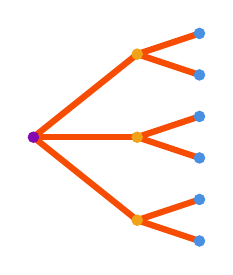
\begin{tikzpicture}[x=0.75pt,y=0.75pt,yscale=-1,xscale=1]
%uncomment if require: \path (0,182); %set diagram left start at 0, and has height of 182

%Straight Lines [id:da5808000645086375] 
\draw [color={rgb, 255:red, 246; green, 76; blue, 4 }  ,draw opacity=1 ][line width=2.25]    (360,70) -- (390,80) ;
%Straight Lines [id:da18975921226163972] 
\draw [color={rgb, 255:red, 246; green, 76; blue, 4 }  ,draw opacity=1 ][line width=2.25]    (390,60) -- (360,70) ;
%Straight Lines [id:da6595221878479601] 
\draw [color={rgb, 255:red, 246; green, 76; blue, 4 }  ,draw opacity=1 ][line width=2.25]    (360,110) -- (390,120) ;
%Straight Lines [id:da5683498370526975] 
\draw [color={rgb, 255:red, 246; green, 76; blue, 4 }  ,draw opacity=1 ][line width=2.25]    (390,100) -- (360,110) ;
%Straight Lines [id:da9165166451633462] 
\draw [color={rgb, 255:red, 246; green, 76; blue, 4 }  ,draw opacity=1 ][line width=2.25]    (360,30) -- (390,40) ;
%Straight Lines [id:da7926013585642647] 
\draw [color={rgb, 255:red, 246; green, 76; blue, 4 }  ,draw opacity=1 ][line width=2.25]    (390,20) -- (360,30) ;
%Straight Lines [id:da7417109803866969] 
\draw [color={rgb, 255:red, 246; green, 76; blue, 4 }  ,draw opacity=1 ][line width=2.25]    (310,70) -- (360,30) ;
%Straight Lines [id:da32862812153335397] 
\draw [color={rgb, 255:red, 246; green, 76; blue, 4 }  ,draw opacity=1 ][line width=2.25]    (310,70) -- (360,70) ;
%Straight Lines [id:da9935618987409959] 
\draw [color={rgb, 255:red, 246; green, 76; blue, 4 }  ,draw opacity=1 ][line width=2.25]    (310,70) -- (360,110) ;
%Shape: Circle [id:dp31789546772639043] 
\draw  [color={rgb, 255:red, 132; green, 9; blue, 175 }  ,draw opacity=1 ][fill={rgb, 255:red, 132; green, 9; blue, 175 }  ,fill opacity=1 ] (307.5,70) .. controls (307.5,68.62) and (308.62,67.5) .. (310,67.5) .. controls (311.38,67.5) and (312.5,68.62) .. (312.5,70) .. controls (312.5,71.38) and (311.38,72.5) .. (310,72.5) .. controls (308.62,72.5) and (307.5,71.38) .. (307.5,70) -- cycle ;
%Shape: Circle [id:dp6750291852439366] 
\draw  [color={rgb, 255:red, 74; green, 144; blue, 226 }  ,draw opacity=1 ][fill={rgb, 255:red, 74; green, 144; blue, 226 }  ,fill opacity=1 ] (387.5,120) .. controls (387.5,118.62) and (388.62,117.5) .. (390,117.5) .. controls (391.38,117.5) and (392.5,118.62) .. (392.5,120) .. controls (392.5,121.38) and (391.38,122.5) .. (390,122.5) .. controls (388.62,122.5) and (387.5,121.38) .. (387.5,120) -- cycle ;
%Shape: Circle [id:dp5494552717190384] 
\draw  [color={rgb, 255:red, 241; green, 163; blue, 23 }  ,draw opacity=1 ][fill={rgb, 255:red, 241; green, 163; blue, 23 }  ,fill opacity=1 ] (357.5,110) .. controls (357.5,108.62) and (358.62,107.5) .. (360,107.5) .. controls (361.38,107.5) and (362.5,108.62) .. (362.5,110) .. controls (362.5,111.38) and (361.38,112.5) .. (360,112.5) .. controls (358.62,112.5) and (357.5,111.38) .. (357.5,110) -- cycle ;
%Shape: Circle [id:dp8629159729730512] 
\draw  [color={rgb, 255:red, 74; green, 144; blue, 226 }  ,draw opacity=1 ][fill={rgb, 255:red, 74; green, 144; blue, 226 }  ,fill opacity=1 ] (387.5,80) .. controls (387.5,78.62) and (388.62,77.5) .. (390,77.5) .. controls (391.38,77.5) and (392.5,78.62) .. (392.5,80) .. controls (392.5,81.38) and (391.38,82.5) .. (390,82.5) .. controls (388.62,82.5) and (387.5,81.38) .. (387.5,80) -- cycle ;
%Shape: Circle [id:dp6642418585732942] 
\draw  [color={rgb, 255:red, 241; green, 163; blue, 23 }  ,draw opacity=1 ][fill={rgb, 255:red, 241; green, 163; blue, 23 }  ,fill opacity=1 ] (357.5,70) .. controls (357.5,68.62) and (358.62,67.5) .. (360,67.5) .. controls (361.38,67.5) and (362.5,68.62) .. (362.5,70) .. controls (362.5,71.38) and (361.38,72.5) .. (360,72.5) .. controls (358.62,72.5) and (357.5,71.38) .. (357.5,70) -- cycle ;
%Shape: Circle [id:dp6409499135433837] 
\draw  [color={rgb, 255:red, 74; green, 144; blue, 226 }  ,draw opacity=1 ][fill={rgb, 255:red, 74; green, 144; blue, 226 }  ,fill opacity=1 ] (387.5,60) .. controls (387.5,58.62) and (388.62,57.5) .. (390,57.5) .. controls (391.38,57.5) and (392.5,58.62) .. (392.5,60) .. controls (392.5,61.38) and (391.38,62.5) .. (390,62.5) .. controls (388.62,62.5) and (387.5,61.38) .. (387.5,60) -- cycle ;
%Shape: Circle [id:dp6267335925860115] 
\draw  [color={rgb, 255:red, 74; green, 144; blue, 226 }  ,draw opacity=1 ][fill={rgb, 255:red, 74; green, 144; blue, 226 }  ,fill opacity=1 ] (387.5,100) .. controls (387.5,98.62) and (388.62,97.5) .. (390,97.5) .. controls (391.38,97.5) and (392.5,98.62) .. (392.5,100) .. controls (392.5,101.38) and (391.38,102.5) .. (390,102.5) .. controls (388.62,102.5) and (387.5,101.38) .. (387.5,100) -- cycle ;
%Shape: Circle [id:dp35239961388070173] 
\draw  [color={rgb, 255:red, 74; green, 144; blue, 226 }  ,draw opacity=1 ][fill={rgb, 255:red, 74; green, 144; blue, 226 }  ,fill opacity=1 ] (387.5,40) .. controls (387.5,38.62) and (388.62,37.5) .. (390,37.5) .. controls (391.38,37.5) and (392.5,38.62) .. (392.5,40) .. controls (392.5,41.38) and (391.38,42.5) .. (390,42.5) .. controls (388.62,42.5) and (387.5,41.38) .. (387.5,40) -- cycle ;
%Shape: Circle [id:dp6520996479300846] 
\draw  [color={rgb, 255:red, 241; green, 163; blue, 23 }  ,draw opacity=1 ][fill={rgb, 255:red, 241; green, 163; blue, 23 }  ,fill opacity=1 ] (357.5,30) .. controls (357.5,28.62) and (358.62,27.5) .. (360,27.5) .. controls (361.38,27.5) and (362.5,28.62) .. (362.5,30) .. controls (362.5,31.38) and (361.38,32.5) .. (360,32.5) .. controls (358.62,32.5) and (357.5,31.38) .. (357.5,30) -- cycle ;
%Shape: Circle [id:dp39086329664120045] 
\draw  [color={rgb, 255:red, 74; green, 144; blue, 226 }  ,draw opacity=1 ][fill={rgb, 255:red, 74; green, 144; blue, 226 }  ,fill opacity=1 ] (387.5,20) .. controls (387.5,18.62) and (388.62,17.5) .. (390,17.5) .. controls (391.38,17.5) and (392.5,18.62) .. (392.5,20) .. controls (392.5,21.38) and (391.38,22.5) .. (390,22.5) .. controls (388.62,22.5) and (387.5,21.38) .. (387.5,20) -- cycle ;




\end{tikzpicture}
%     \vspace{-1cm}
%     \caption{$(3, 2)$ tree graph state}
%     \label{fig:3_3_tree}
% \end{wrapfigure}

Beginning from the final state derived from \cref{eq:tree_implementation}, by replicating the process outlined in \cref{eq:1_branch_implementation} to generate another branch, we could extend the implementation to create a generalized $(2, 2)$ tree graph state, thereby enabling the implementation of a $(n, 2)$ tree state.

As an example let us consider a $(3, 2)$ tree state (see \cref{fig:3_3_tree}).
It can be implemented using the following sequence of gates.
In the first gate, the instruction is simply to execute the same operations as those described in \cref{eq:tree_implementation}.

\begin{equation}
    \begin{quantikz}[transparent]
        \lstick{$\ket{0}_{S1}$} & \gate[8]{\text{\cref{eq:tree_implementation}}} & \qw & \qw & \qw & \ctrl{1} & \qw & \qw & \qw & \qw \\
        \lstick{$\ket{0}_{S2}$} & \qw & \gate{Y_+} & \ctrl{7} & \gate{Y_-} & \control{} & \ctrl{8} & \gate{Y_+} & \swap{9} & \qw \\
        \lstick{$\ket{0}_{P1}$} & \qw & \qw & \qw & \qw & \qw & \qw & \qw & \qw & \qw \\
        \lstick{$\ket{0}_{P2}$} & \qw & \qw & \qw & \qw & \qw & \qw & \qw & \qw & \qw \\
        \lstick{$\ket{0}_{P3}$} & \qw & \qw & \qw & \qw & \qw & \qw & \qw & \qw & \qw \\
        \lstick{$\ket{0}_{P4}$} & \qw & \qw & \qw & \qw & \qw & \qw & \qw & \qw & \qw \\
        \lstick{$\ket{0}_{P5}$} & \qw & \qw & \qw & \qw & \qw & \qw & \qw & \qw & \qw \\
        \lstick{$\ket{0}_{P6}$} & \qw & \qw & \qw & \qw & \qw & \qw & \qw & \qw & \qw \\
        \lstick{$\ket{0}_{P7}$} & \qw & \qw & \targ{} & \qw & \qw & \qw & \qw & \qw & \qw \\
        \lstick{$\ket{0}_{P8}$} & \qw & \qw & \qw & \qw & \qw & \targ{} & \qw & \qw & \qw \\
        \lstick{$\ket{0}_{P9}$} & \qw & \qw & \qw & \qw & \qw & \qw & \qw & \targX{} & \qw        
    \end{quantikz}
\end{equation}


%\section{(n, 3) Tree Graph State}

\chapter*{Conclusions}
\markboth{CONCLUSIONS}{}
\addcontentsline{toc}{chapter}{Conclusions}
\label{chap:conclusions}

Here you write the conclusions



%Print bibliography
\printbibliography[heading=bibintoc]

\thispagestyle{plain}

\end{document}